\documentclass[aspectratio=169]{beamer}

\usepackage{graphicx}
\usepackage{natbib}
\usepackage{xmpmulti}
\usepackage{animate}
\usepackage[english]{babel}
\usepackage[latin1]{inputenc}
\usepackage{times}
\usepackage[T1]{fontenc}
\usefonttheme{serif}

\beamertemplatenavigationsymbolsempty
\useoutertheme{shadow}
\setbeamertemplate{headline}{}

\title[HDR soutenance]{Rivers and Melt: Exploring how physical processes are stored in the geological record}

\author[Armitage]{{\bf John Armitage}\inst{1}}
\institute[IFPEN]
{
  \inst{1}
  IFP Energies Nouvelles, France
}
\date[20 May]{HDR soutenance 20/5/2021}
\subject{Everything}

\begin{document}

\newcommand{\SubItem}[1]{
    {\setlength\itemindent{15pt} \item[-] #1}
}

{
\usebackgroundtemplate{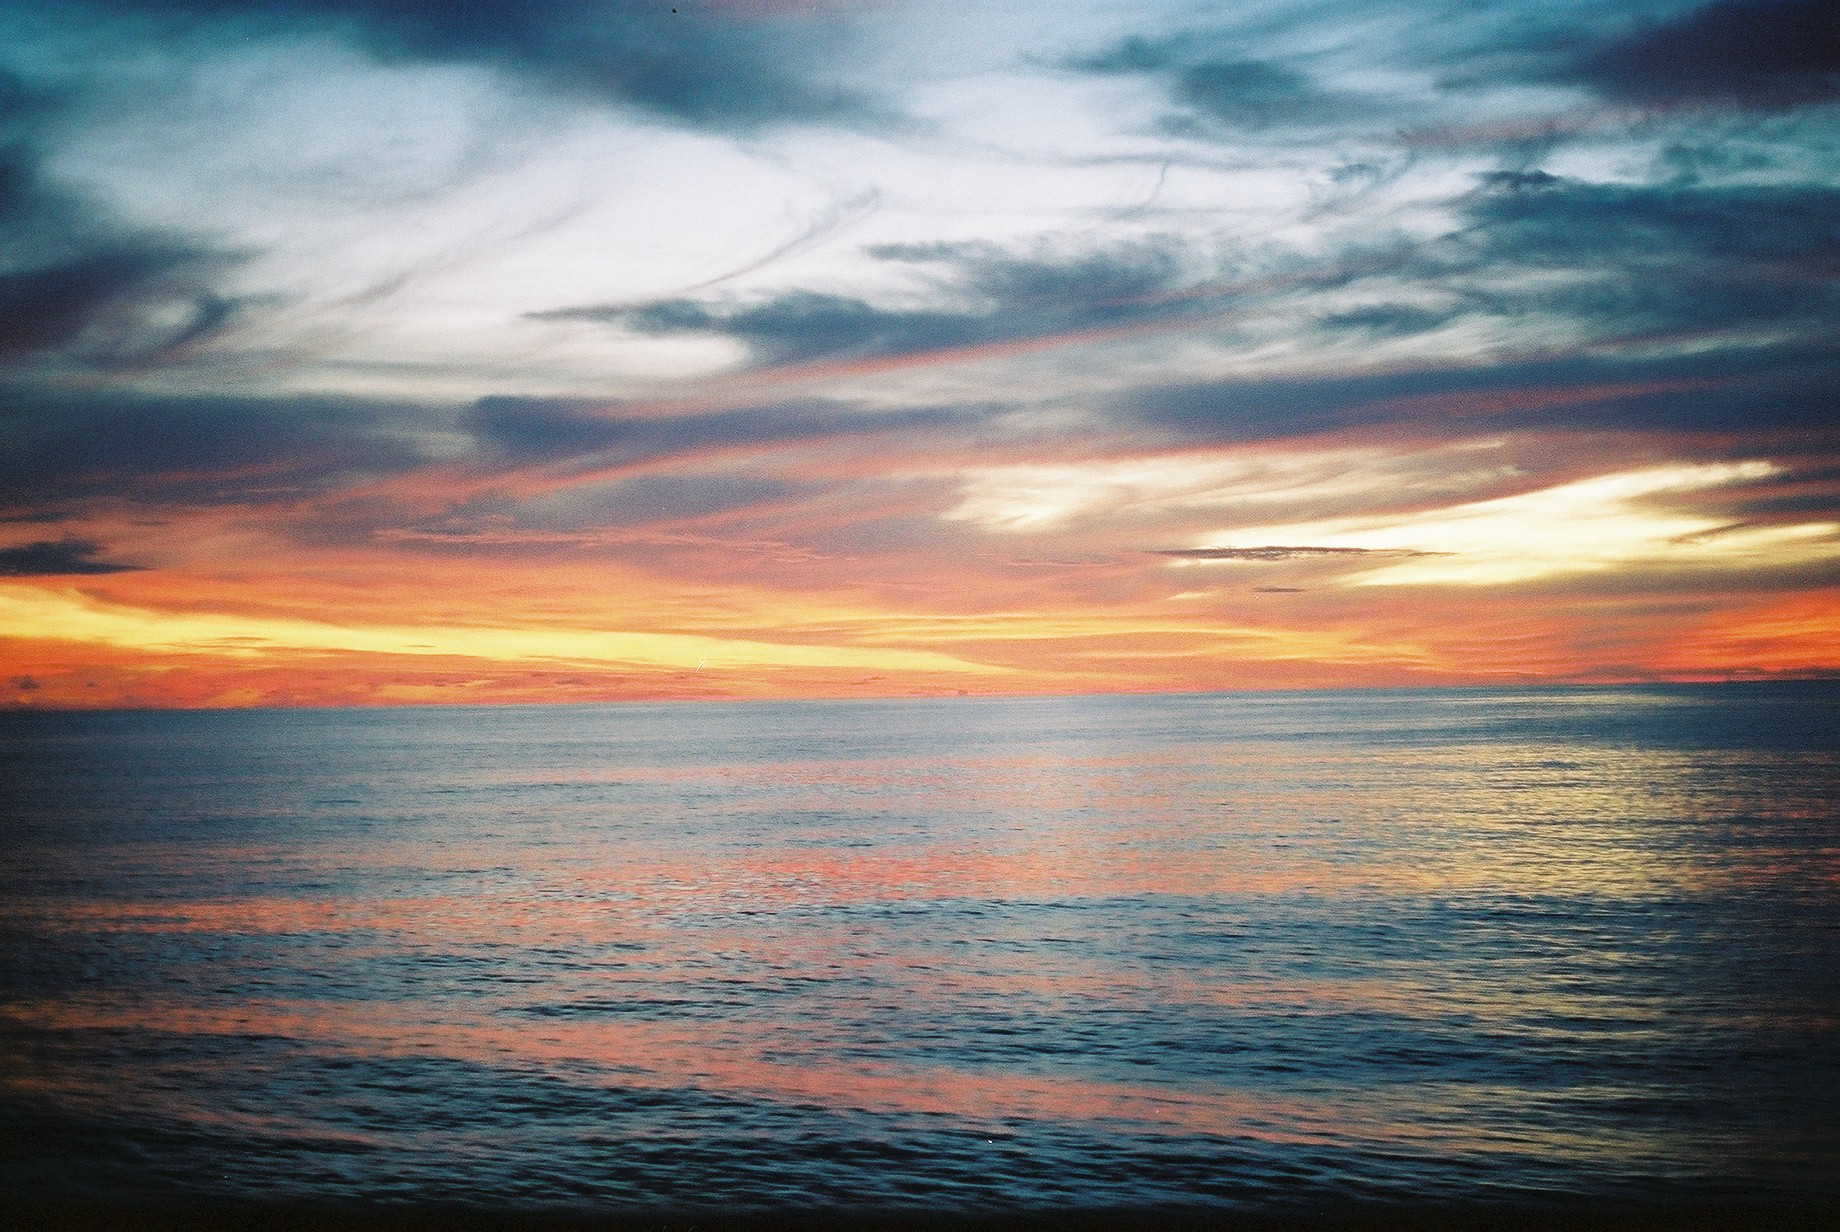
\includegraphics[width=\paperwidth]{./pictures/sea.jpg}}
\begin{frame}
  \titlepage
\end{frame}
}

\section{Background}

\begin{frame}
    \frametitle{My background}
    \begin{itemize}
        \item[-]{PhD in Geophysics - National Oceanography Centre, University of Southampton, UK \\
              Title `How Does Melting Affect Continental Rift Development ?' \\
              \bf{2004 - 2009}}
        \item[-]{Masters in Oceanography - National Oceanography Centre, University of Southampton, UK \\
              Masters Project Title `Dissolution of Silica from Antarctic Continental Shelf Sea Sediments' \\
              \bf{2003 - 2004}}
    \end{itemize}
\end{frame}

{
\usebackgroundtemplate{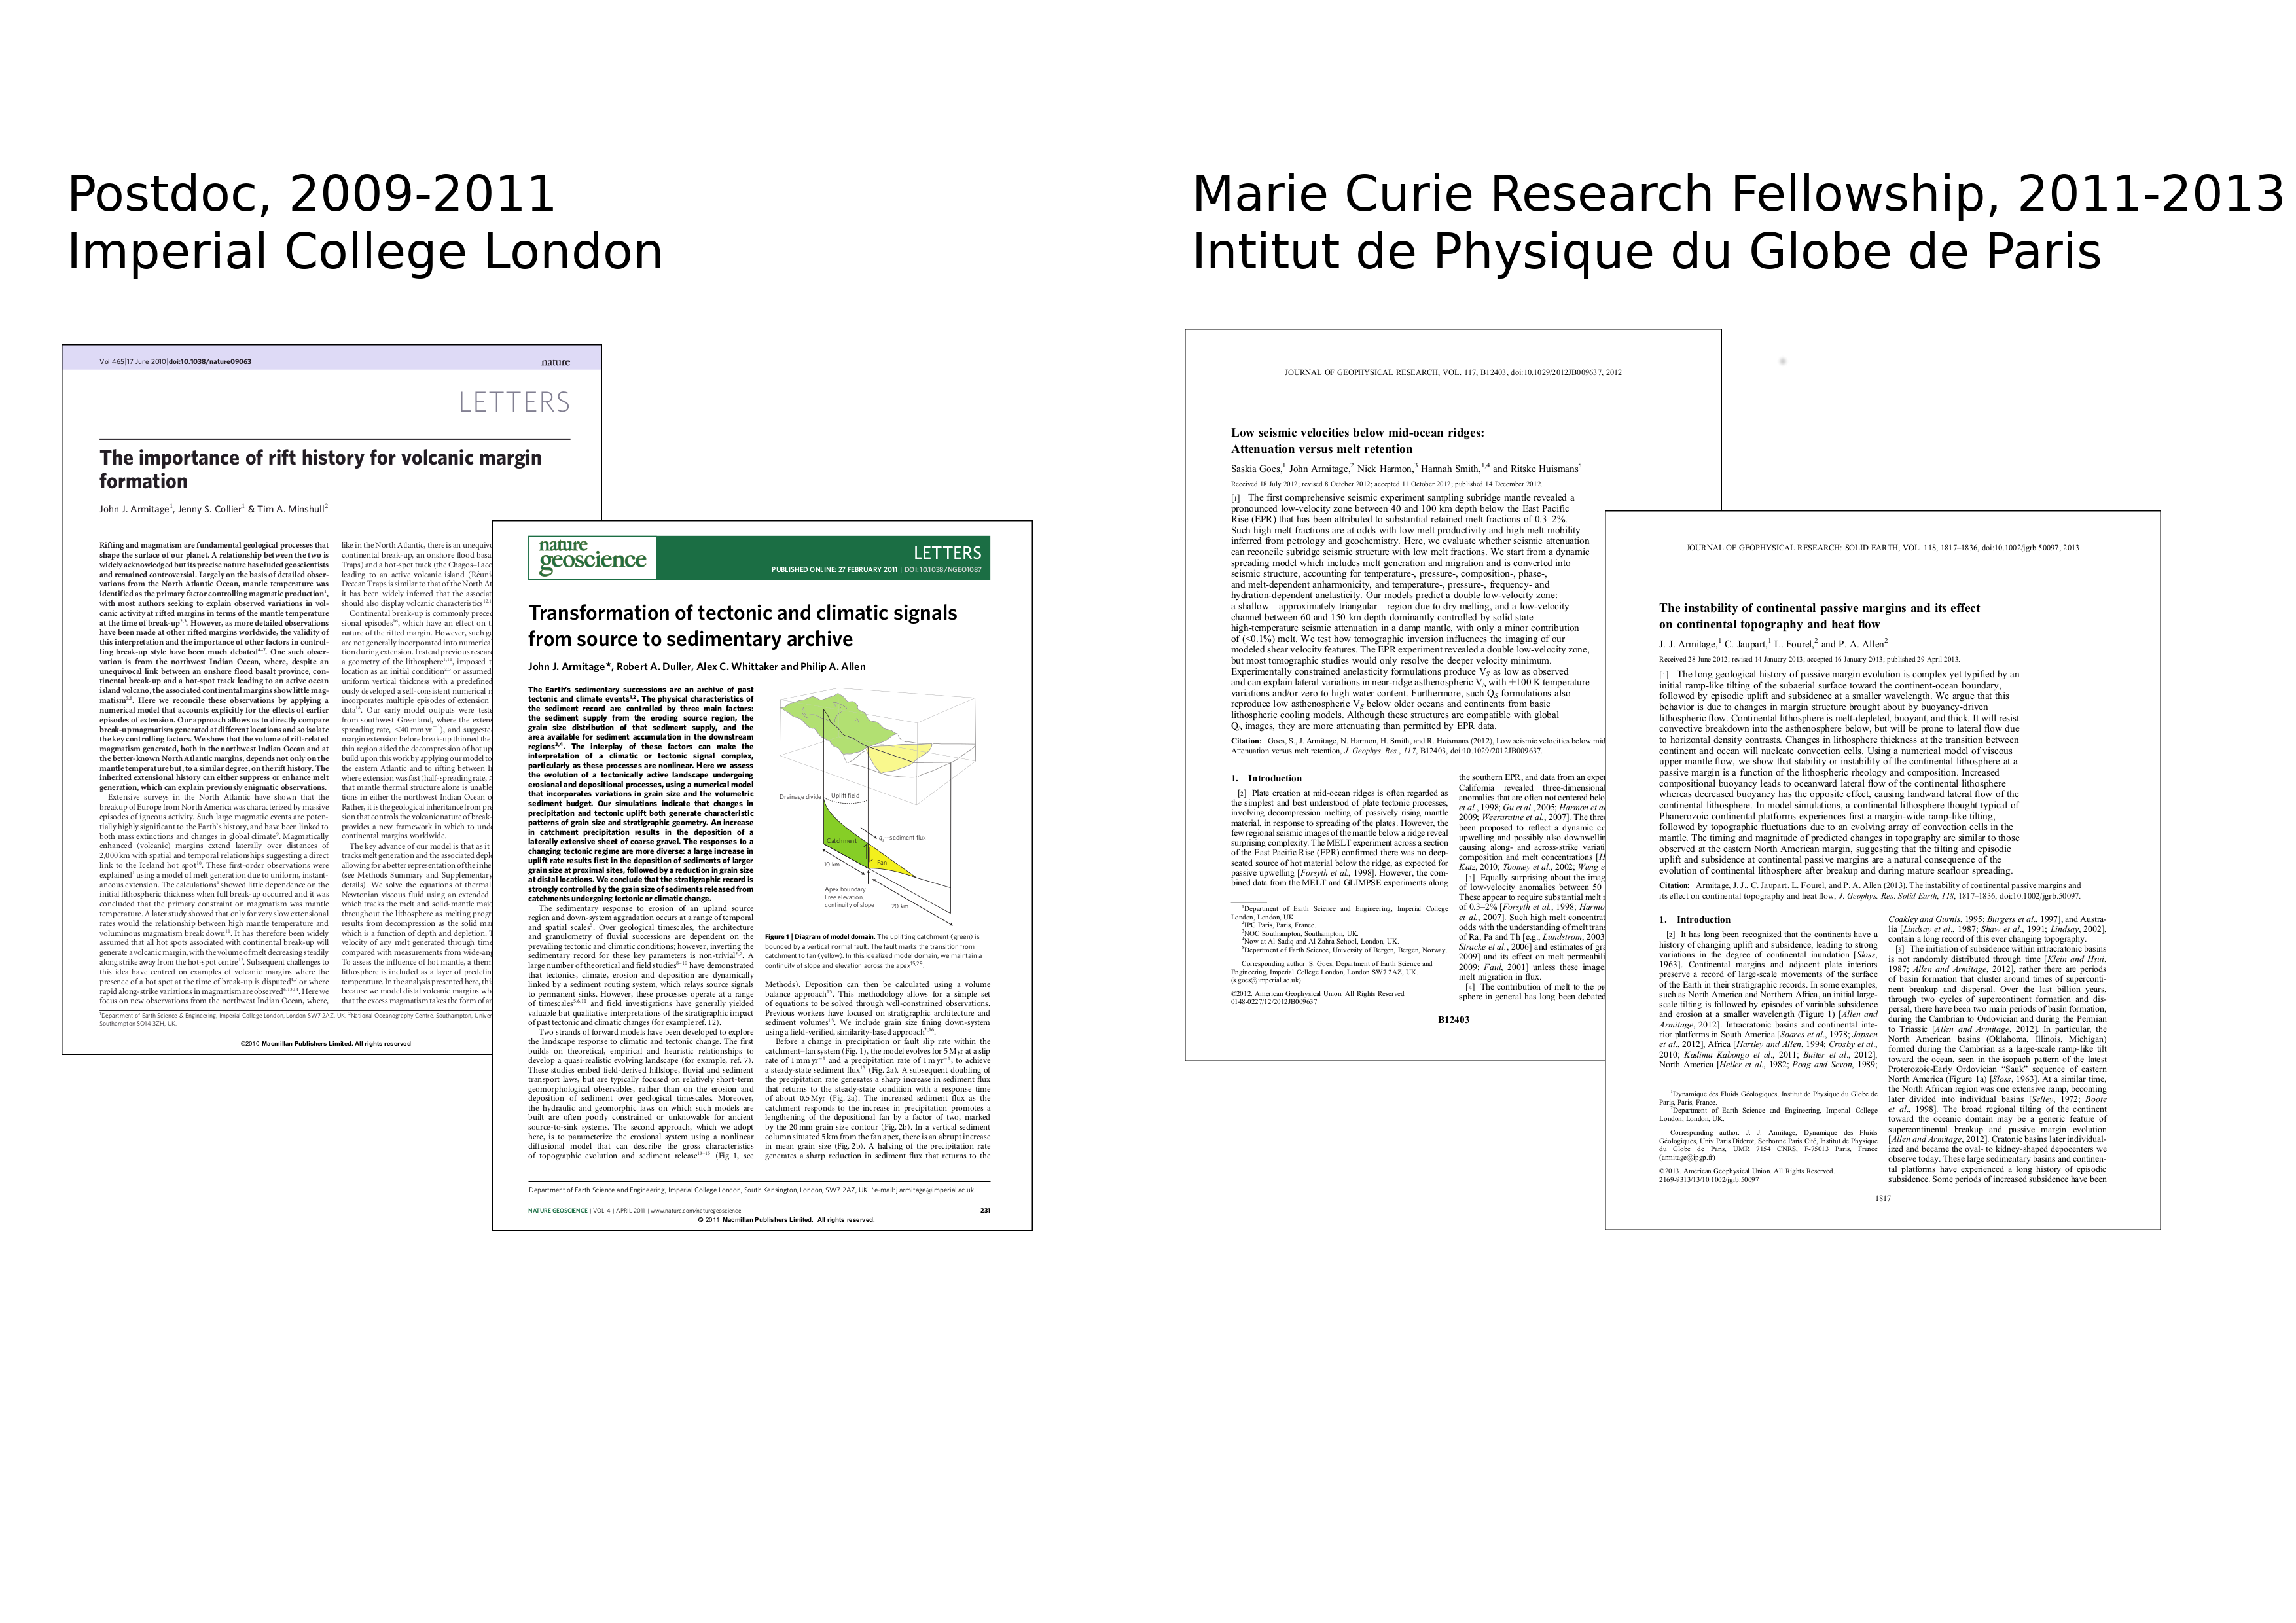
\includegraphics[width=\paperwidth]{./pictures/postdoc12.png}}
\begin{frame}
    \frametitle{Research Positions}
\end{frame}
}

{
\usebackgroundtemplate{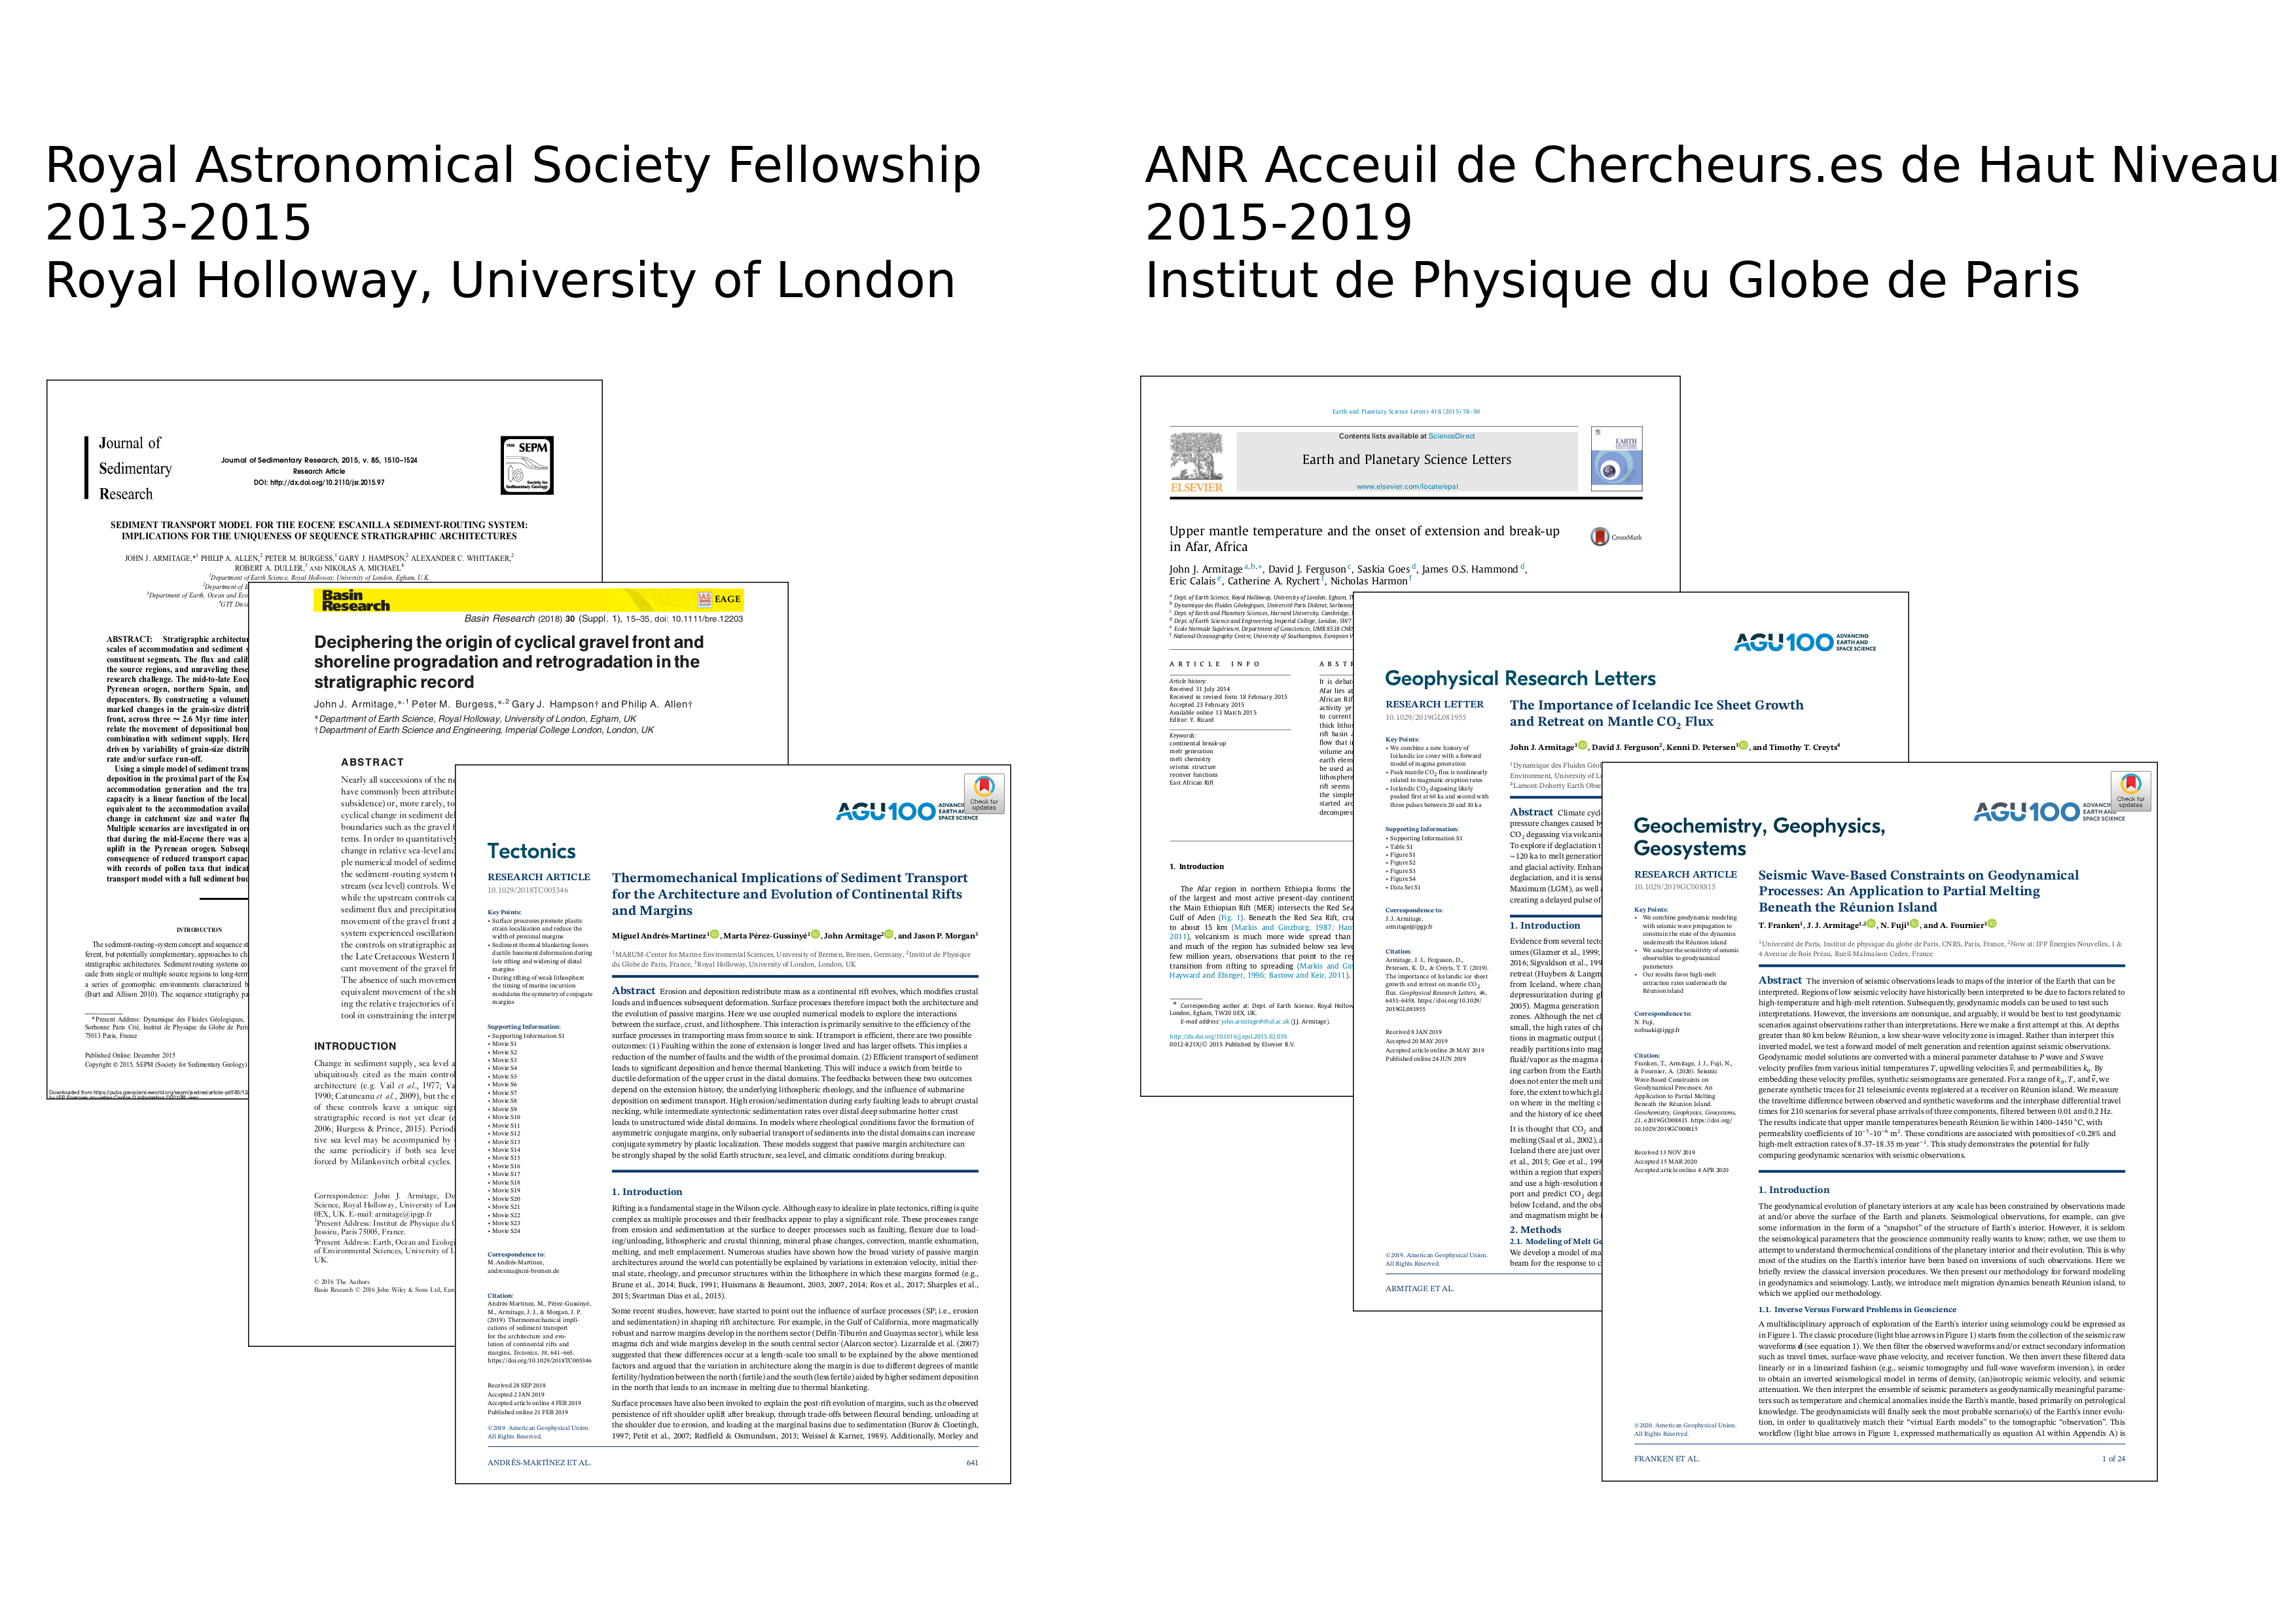
\includegraphics[width=\paperwidth]{./pictures/postdoc34.png}}
\begin{frame}
    \frametitle{Research Positions}
\end{frame}
}

\begin{frame}
    \frametitle{Got a job in DevOps}
    \centering
    
\includegraphics[width=0.7\paperwidth]{./pictures/kubernetes.png}
\end{frame}

\begin{frame}
    \frametitle{Ing{\'e}nieur de Recherche, IFP Energies Nouvelles}
    \begin{itemize}
        \item[-]{Develop novel methods for sediment transport for applications from risk management to exploration}
    \end{itemize}
    \centering
    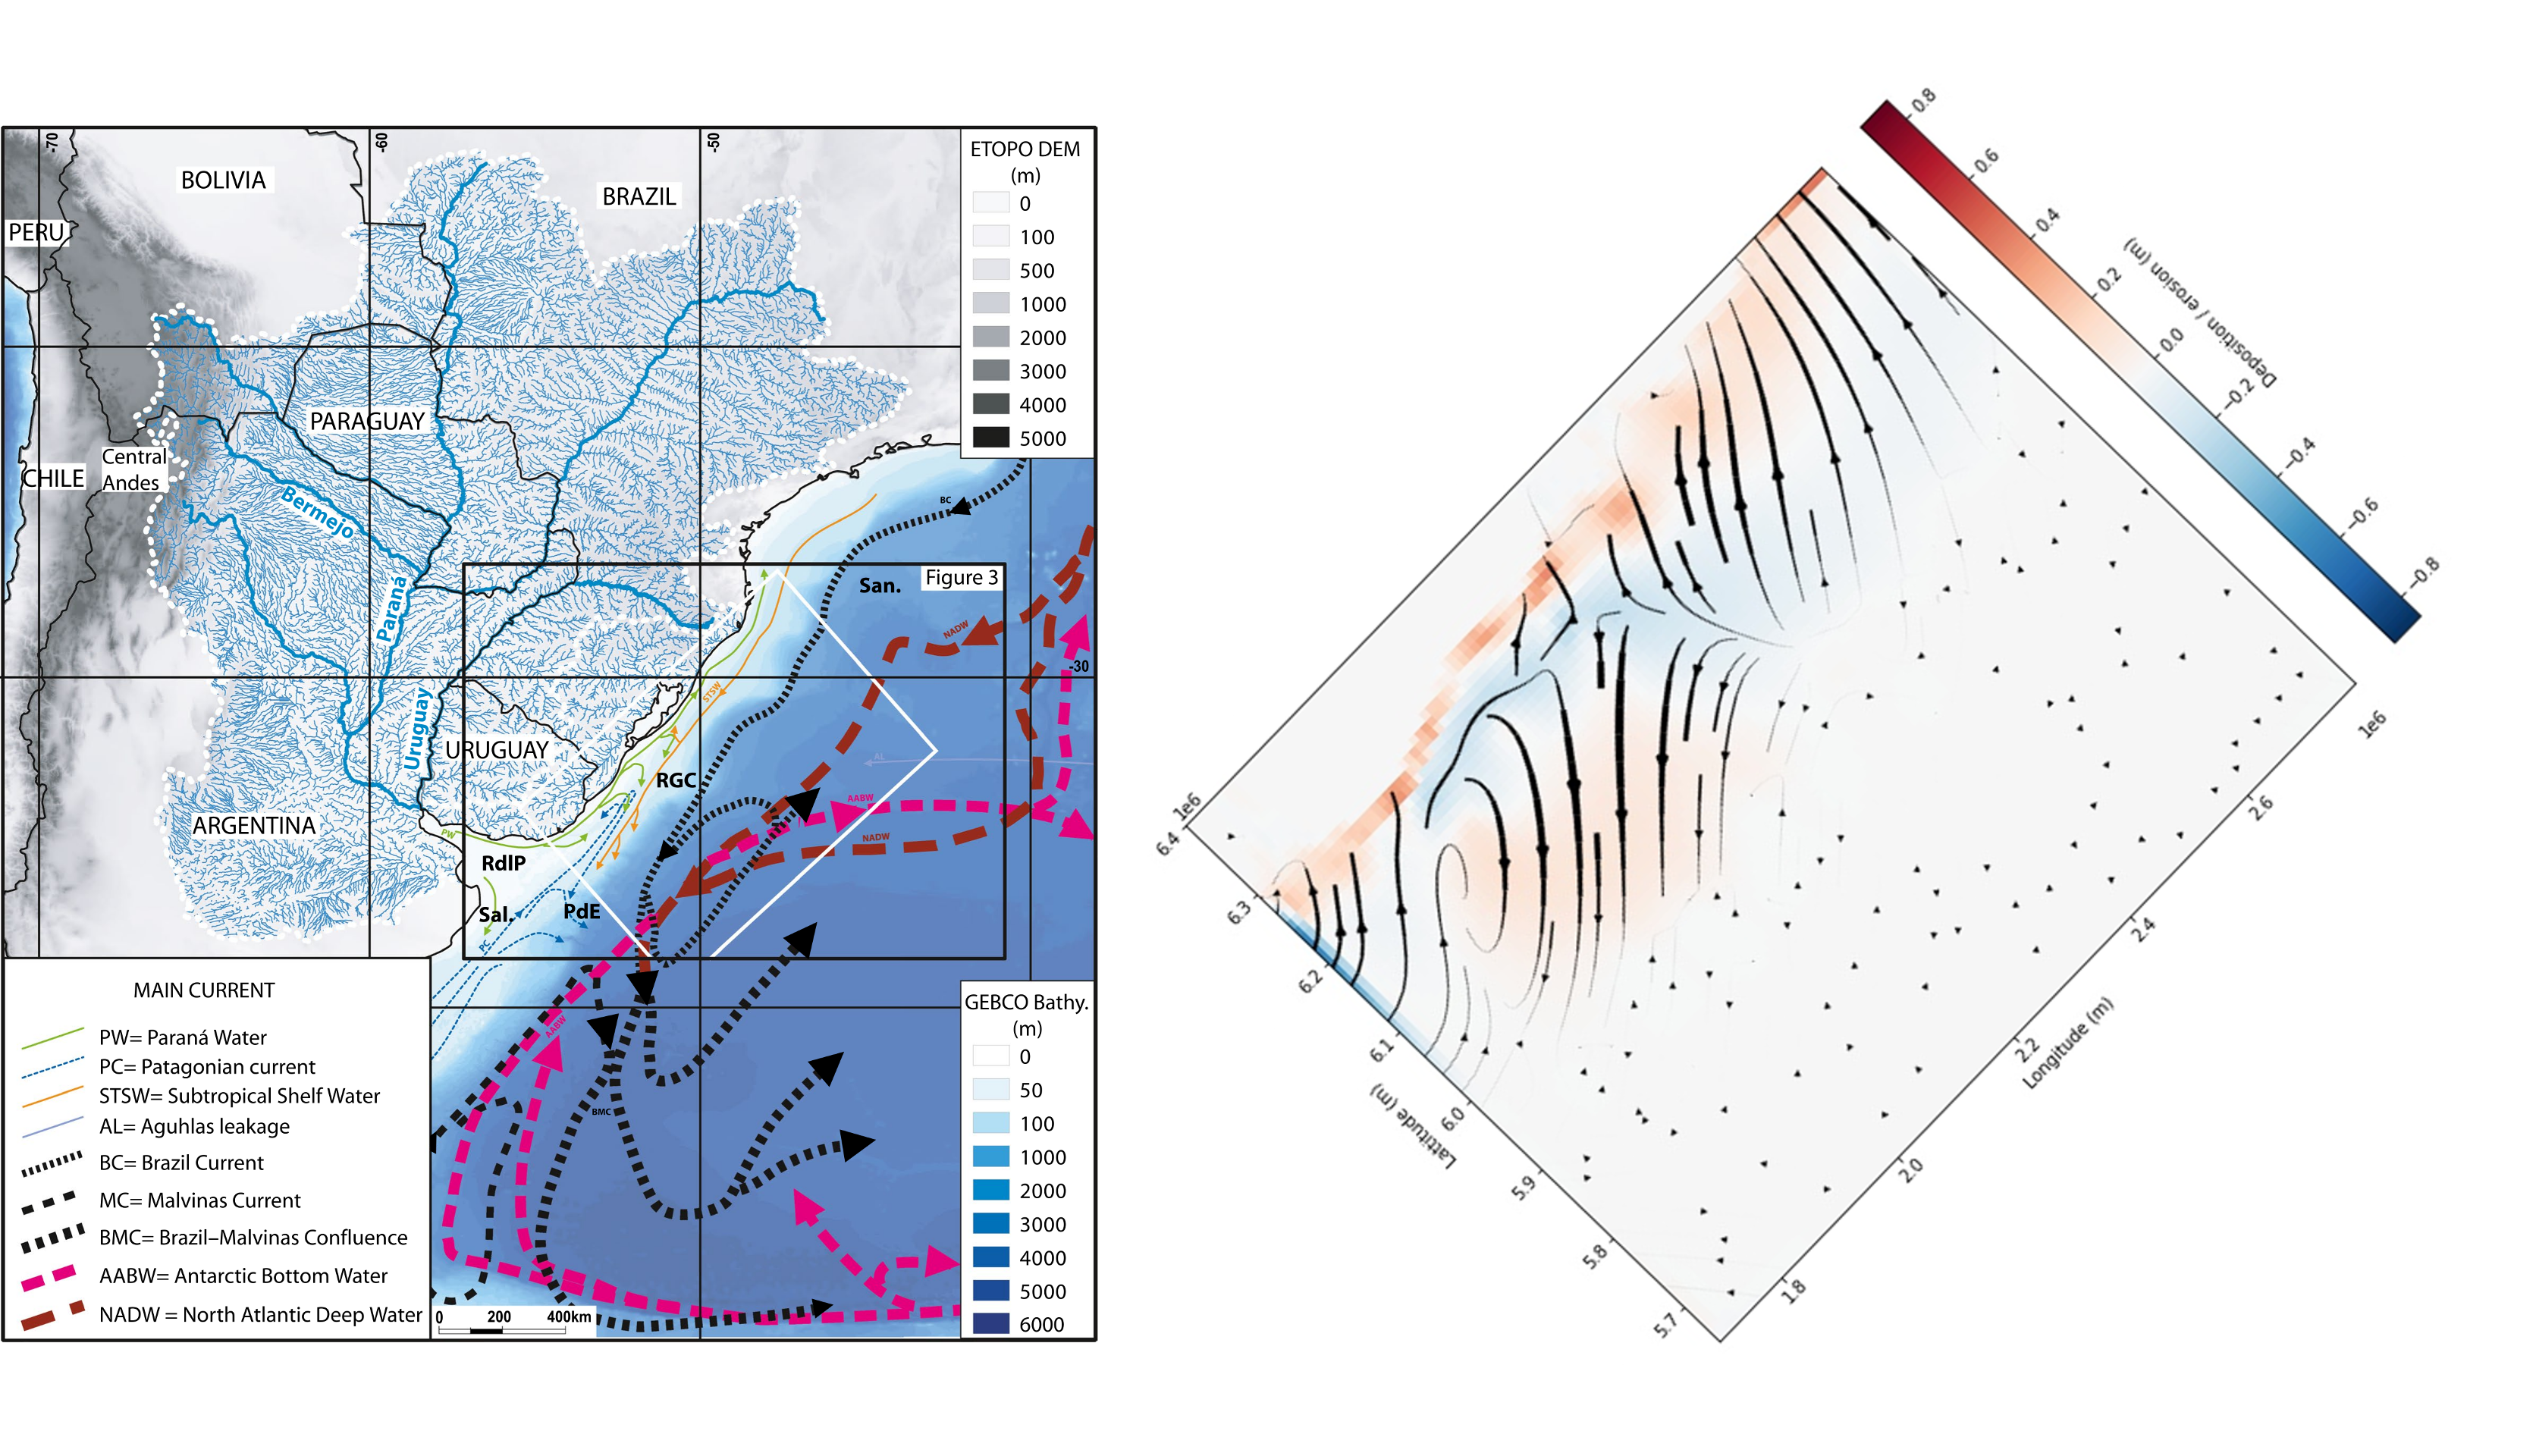
\includegraphics[width=0.6\paperwidth]{./pictures/bottom-currents.png}
\end{frame}

\begin{frame}
    \frametitle{Ing{\'e}nieur de Recherche, IFP Energies Nouvelles}
    \begin{itemize}
        \item[-]{Explore the linking between surface and sub-surface processes}
    \end{itemize}
    \centering
    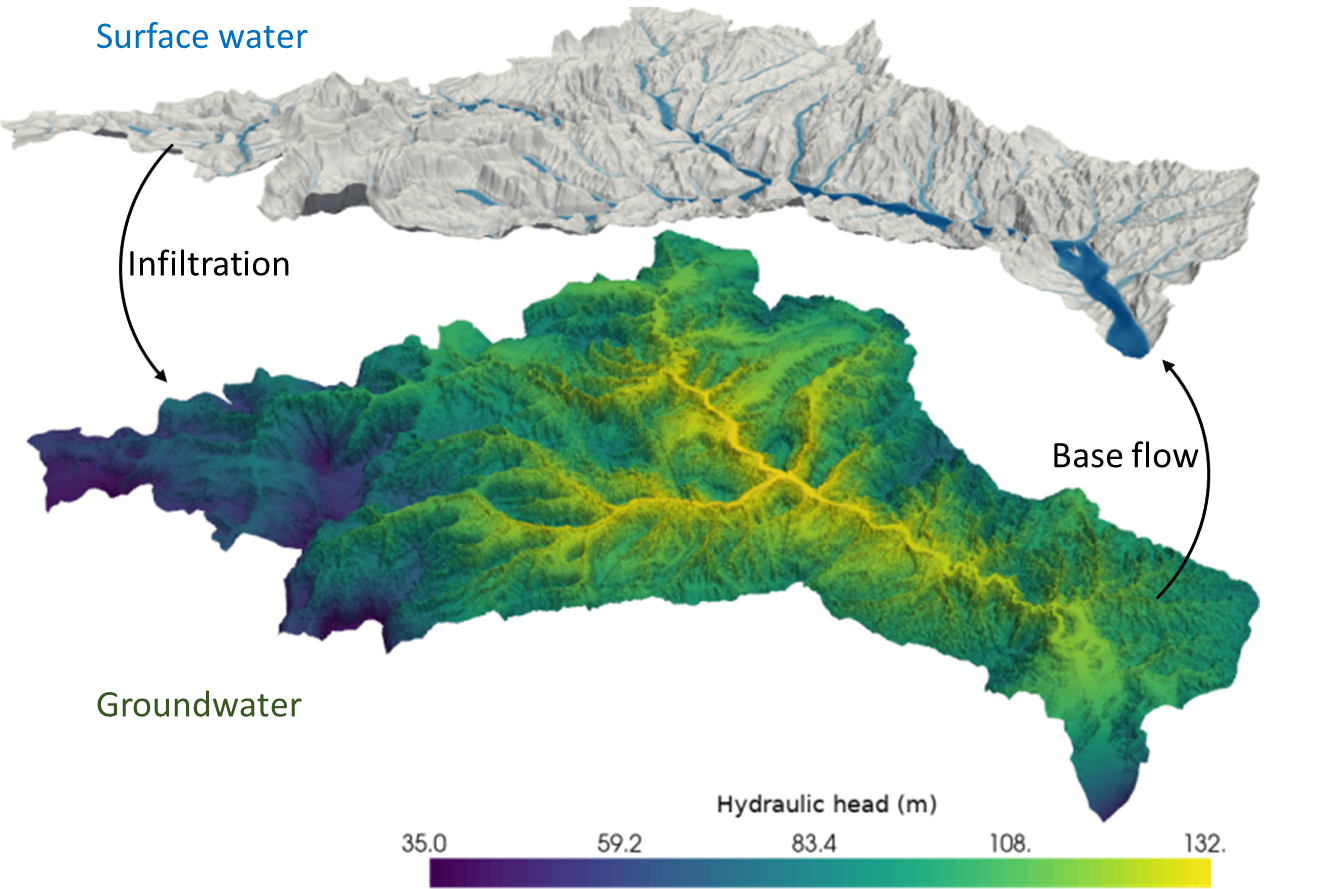
\includegraphics[width=0.6\paperwidth]{./pictures/graphic1.png}
\end{frame}

\begin{frame}
    \frametitle{A career in numbers}
    \begin{itemize}
        \item[-]{{\bf 2020 - present} Ing{\'e}nieur de Recherche at IFP Energies Nouvelles}
        \item[-]{{\bf37} Publications}
        \item[-]{{\bf3} PhD students supervised: \\
              2012-2017: Chandra Taposeea - co-supervised with Jenny Collier, Imperial College London. \\
              2014-2018: Sam Brooke - co-supervised with Alex Whittaker, Imperial College London. \\
              2016-2019: Thijs Franken - co-supervised with Nobu Fuji \& Alexandre Fournier, IPGP.}
        \item[-]{{\bf1} PhD student starting: \\
              2021-2024: Groundwater project with Niels Hovius \& Christoff Andremann, GFZ}
        \item[-]{{\bf3} Research grants: \\
              EU Marie Curie Fellowship, Royal Astronomical Society Research Fellowship, ANR Acceuil de chercheurs$\cdot$es de haute niveau.}
    \end{itemize}
\end{frame}

\section{Part 1: Melt}

{
\usebackgroundtemplate{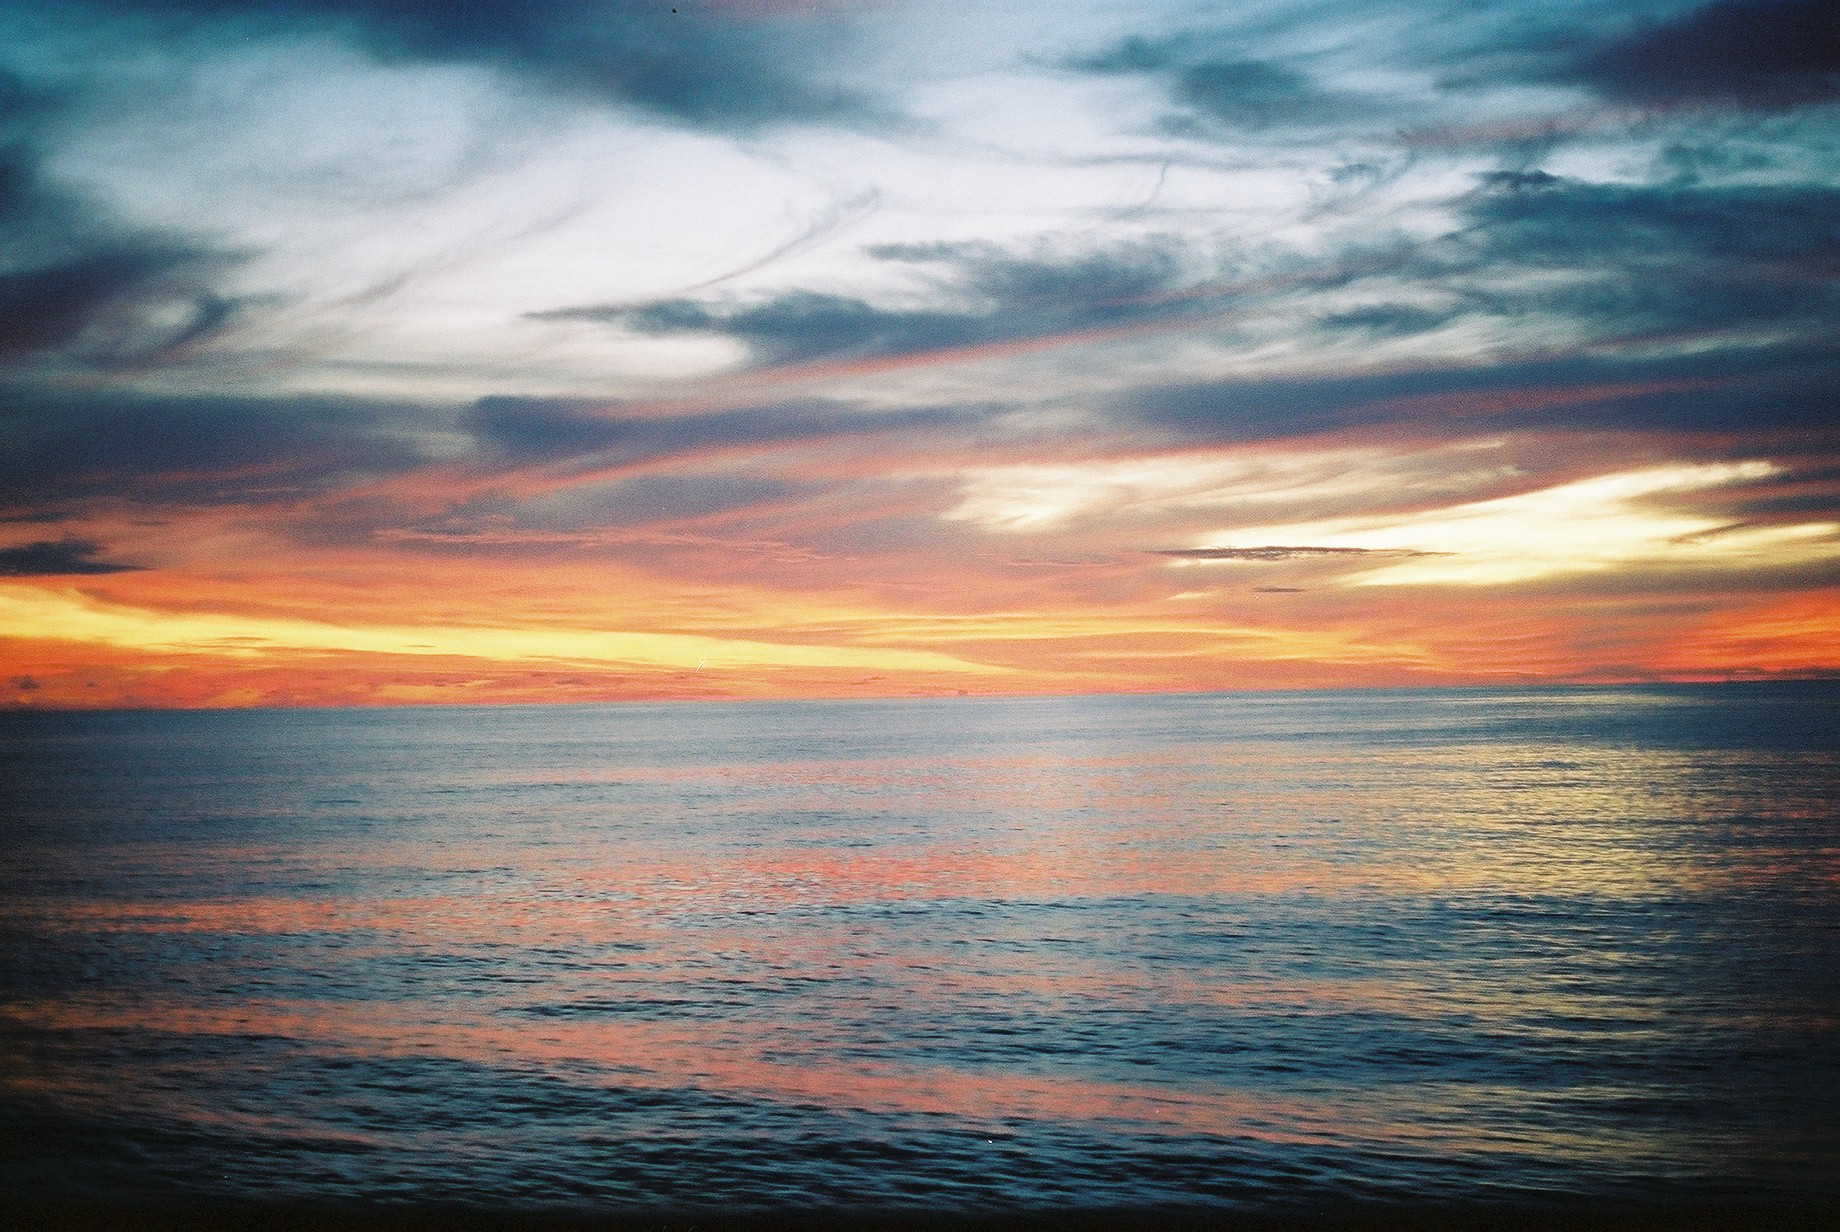
\includegraphics[width=\paperwidth]{./pictures/sea.jpg}}
\begin{frame}
    \frametitle{Part 1: Melt}
\end{frame}
}

\subsection{Upper mantle instabilities}

\begin{frame}
    \frametitle{Part 1.1: Upper mantle structure below zones of volcanism}
    \begin{figure}
        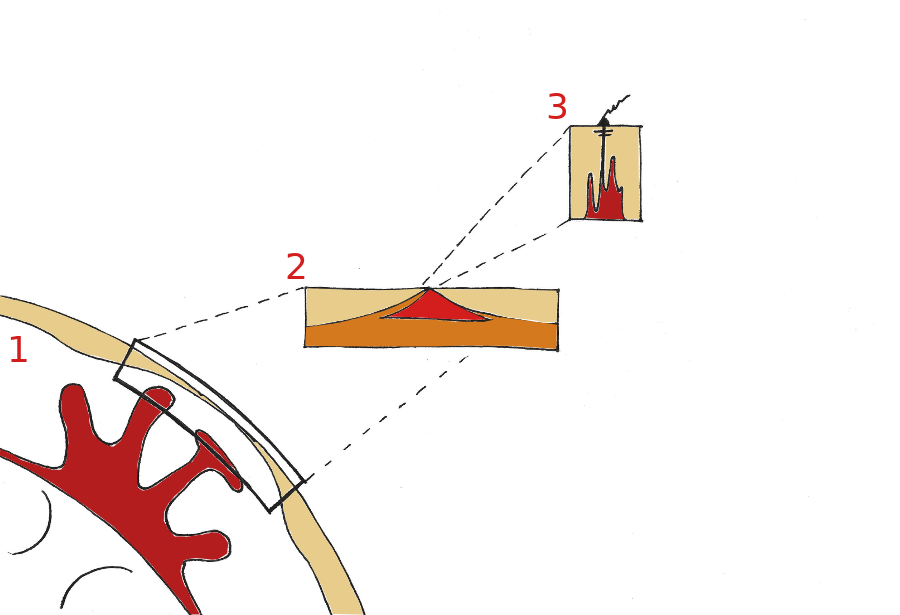
\includegraphics[height=0.9\paperheight]{./pictures/drawing.png}
    \end{figure}
\end{frame}

\begin{frame}
    \frametitle{Elevated mantle temperature leads to volcanism}
    \begin{figure}
        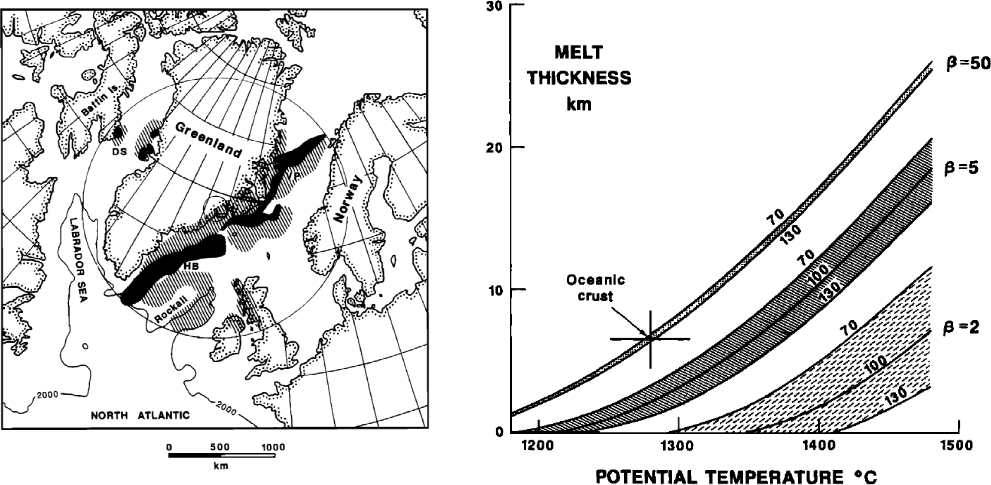
\includegraphics[height=0.6\paperheight]{./figures/mckenzie.png}
        \caption{North Atlantic volcanism is because the mantle was hot \citep{white-1995}.}
    \end{figure}
\end{frame}

\begin{frame}
    \frametitle{Northern East African Rift}
    \begin{figure}
        \includegraphics[height=0.7\paperheight]{./figures/afar-crust-mantle.png}
        \caption{Location of basaltic intrusions and lava flows correlate with deep low seismic velocity anomalies.}
    \end{figure}
\end{frame}

\begin{frame}
    \frametitle{Seismic structure below the Northern East African Rift}
    \begin{figure}
        \vspace{-0.3cm}
        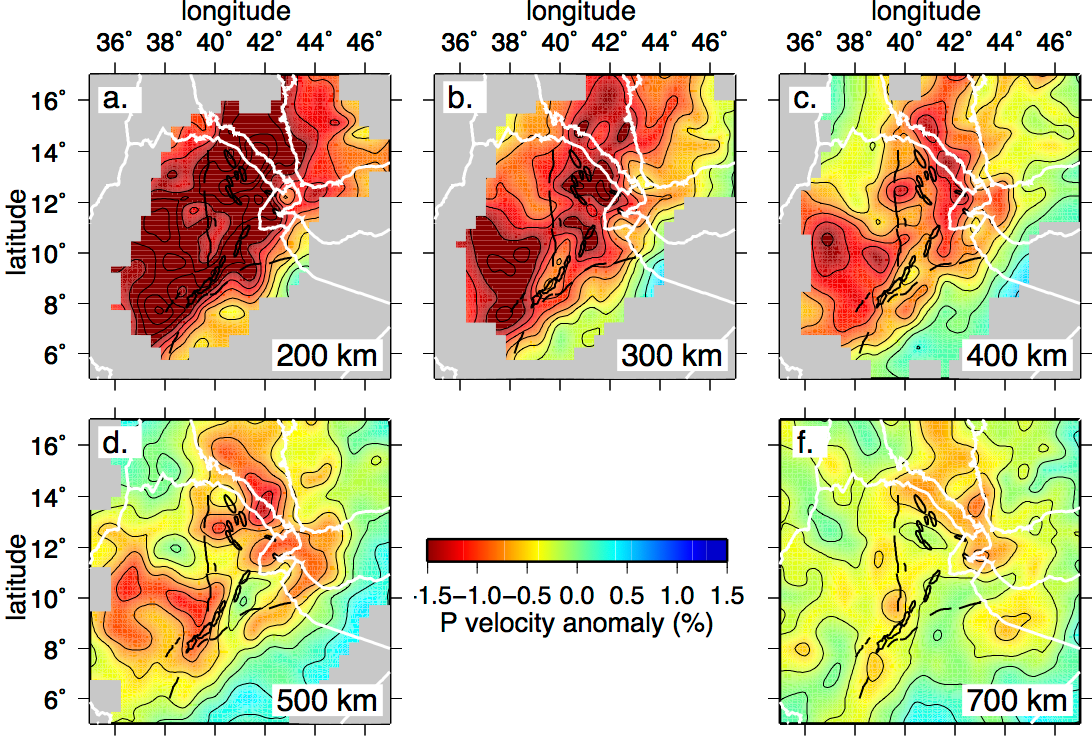
\includegraphics[height=0.7\paperheight]{./figures/civiero-2016.png}
        \caption{The tomographic model of \cite{civiero-etal-2016} suggests multiple upper mantle instabilities}
    \end{figure}
\end{frame}

\begin{frame}
    \frametitle{Seismic structure below the Northern East African Rift}
    \begin{figure}
        \vspace{-0.3cm}
        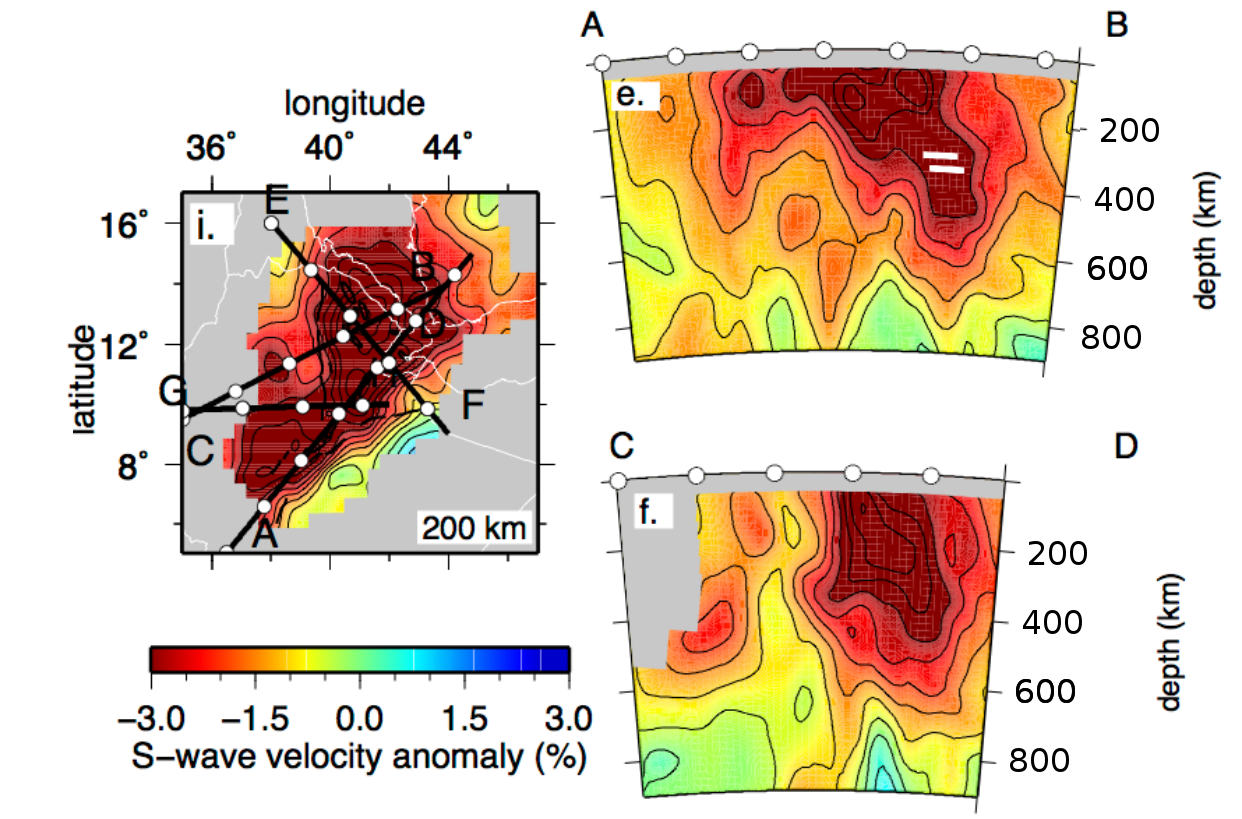
\includegraphics[height=0.7\paperheight]{./figures/chiara1.png}
        \caption{The tomographic model of \cite{civiero-etal-2016} suggests multiple upper mantle instabilities}
    \end{figure}
\end{frame}

\begin{frame}
    \frametitle{Secondary plumes or destabilisation?}
    \begin{figure}
        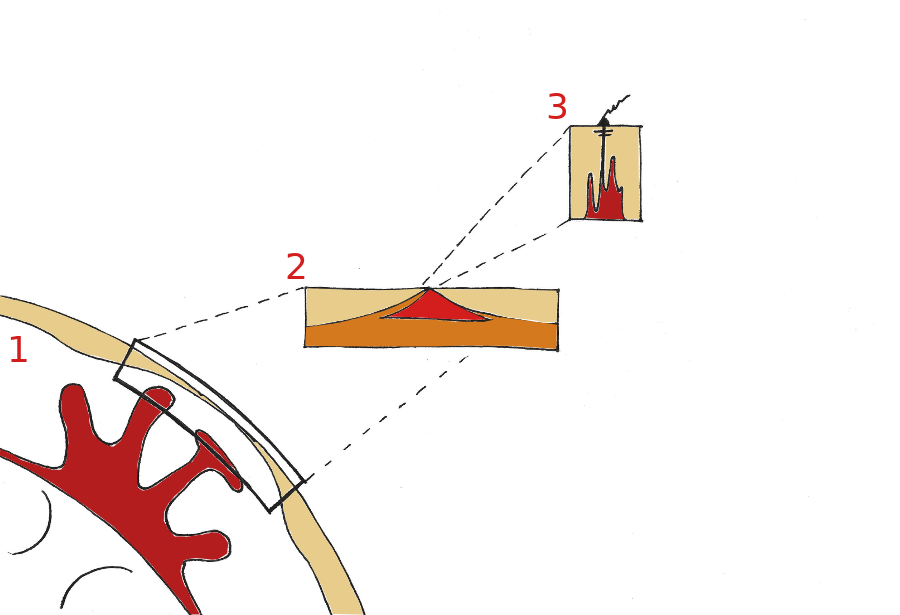
\includegraphics[height=0.9\paperheight]{./pictures/drawing.png}
    \end{figure}
\end{frame}

\begin{frame}
    \frametitle{Thermal instabilities driven by hot base}
    \begin{figure}
        \vspace{-.5cm}
        \includegraphics[width=0.85\paperwidth]{./figures/Newt100/{dT1.0741_4x4_Newt_Ra6e6_0}.png}
        \caption{Thermal instabilities driven by a $100\rm\,^{\circ}C$ hot base. Newtonian rheology, $T_{P}=1350\rm\,^{\circ}C$; $Ra = 6\times10^{6}$.}
    \end{figure}
\end{frame}

\begin{frame}
    \frametitle{Thermal instabilities driven by hot base}
    \begin{figure}
        \vspace{-.5cm}
        \includegraphics[width=0.85\paperwidth]{./figures/Newt100/{dT1.0741_4x4_Newt_Ra6e6_1}.png}
        \caption{Thermal instabilities driven by a $100\rm\,^{\circ}C$ hot base. Newtonian rheology, $T_{P}=1350\rm\,^{\circ}C$; $Ra = 6\times10^{6}$.}
    \end{figure}
\end{frame}

\begin{frame}
    \frametitle{Thermal instabilities driven by hot base}
    \begin{figure}
        \vspace{-.5cm}
        \includegraphics[width=0.85\paperwidth]{./figures/Newt100/{dT1.0741_4x4_Newt_Ra6e6_2}.png}
        \caption{Thermal instabilities driven by a $100\rm\,^{\circ}C$ hot base. Newtonian rheology, $T_{P}=1350\rm\,^{\circ}C$; $Ra = 6\times10^{6}$.}
    \end{figure}
\end{frame}

\begin{frame}
    \frametitle{Thermal instabilities driven by hot base}
    \begin{figure}
        \vspace{-.5cm}
        \includegraphics[width=0.85\paperwidth]{./figures/Newt100/{dT1.0741_4x4_Newt_Ra6e6_3}.png}
        \caption{Thermal instabilities driven by a $100\rm\,^{\circ}C$ hot base. Newtonian rheology, $T_{P}=1350\rm\,^{\circ}C$; $Ra = 6\times10^{6}$.}
    \end{figure}
\end{frame}

\begin{frame}
    \frametitle{Thermal instabilities driven by hot base}
    \begin{figure}
        \vspace{-.5cm}
        \includegraphics[width=0.85\paperwidth]{./figures/Newt100/{dT1.0741_4x4_Newt_Ra6e6_4}.png}
        \caption{Thermal instabilities driven by a $100\rm\,^{\circ}C$ hot base. Newtonian rheology, $T_{P}=1350\rm\,^{\circ}C$; $Ra = 6\times10^{6}$.}
    \end{figure}
\end{frame}

\begin{frame}
    \frametitle{Thermal instabilities driven by hot base}
    \begin{figure}
        \vspace{-.5cm}
        \includegraphics[width=0.85\paperwidth]{./figures/Newt100/{dT1.0741_4x4_Newt_Ra6e6_5}.png}
        \caption{Thermal instabilities driven by a $100\rm\,^{\circ}C$ hot base. Newtonian rheology, $T_{P}=1350\rm\,^{\circ}C$; $Ra = 6\times10^{6}$.}
    \end{figure}
\end{frame}

\begin{frame}
    \frametitle{Thermal instabilities driven by hot base}
    \begin{figure}
        \vspace{-.5cm}
        \includegraphics[width=0.85\paperwidth]{./figures/Newt100/{dT1.0741_4x4_Newt_Ra6e6_6}.png}
        \caption{Thermal instabilities driven by a $100\rm\,^{\circ}C$ hot base. Newtonian rheology, $T_{P}=1350\rm\,^{\circ}C$; $Ra = 6\times10^{6}$.}
    \end{figure}
\end{frame}

\begin{frame}
    \frametitle{Thermal instabilities driven by hot base}
    \begin{figure}
        \vspace{-.5cm}
        \includegraphics[width=0.85\paperwidth]{./figures/Newt100/{dT1.0741_4x4_Newt_Ra6e6_7}.png}
        \caption{Thermal instabilities driven by a $100\rm\,^{\circ}C$ hot base. Newtonian rheology, $T_{P}=1350\rm\,^{\circ}C$; $Ra = 6\times10^{6}$.}
    \end{figure}
\end{frame}

\begin{frame}
    \frametitle{Relationship between Ra and $\lambda$}
    \begin{figure}
        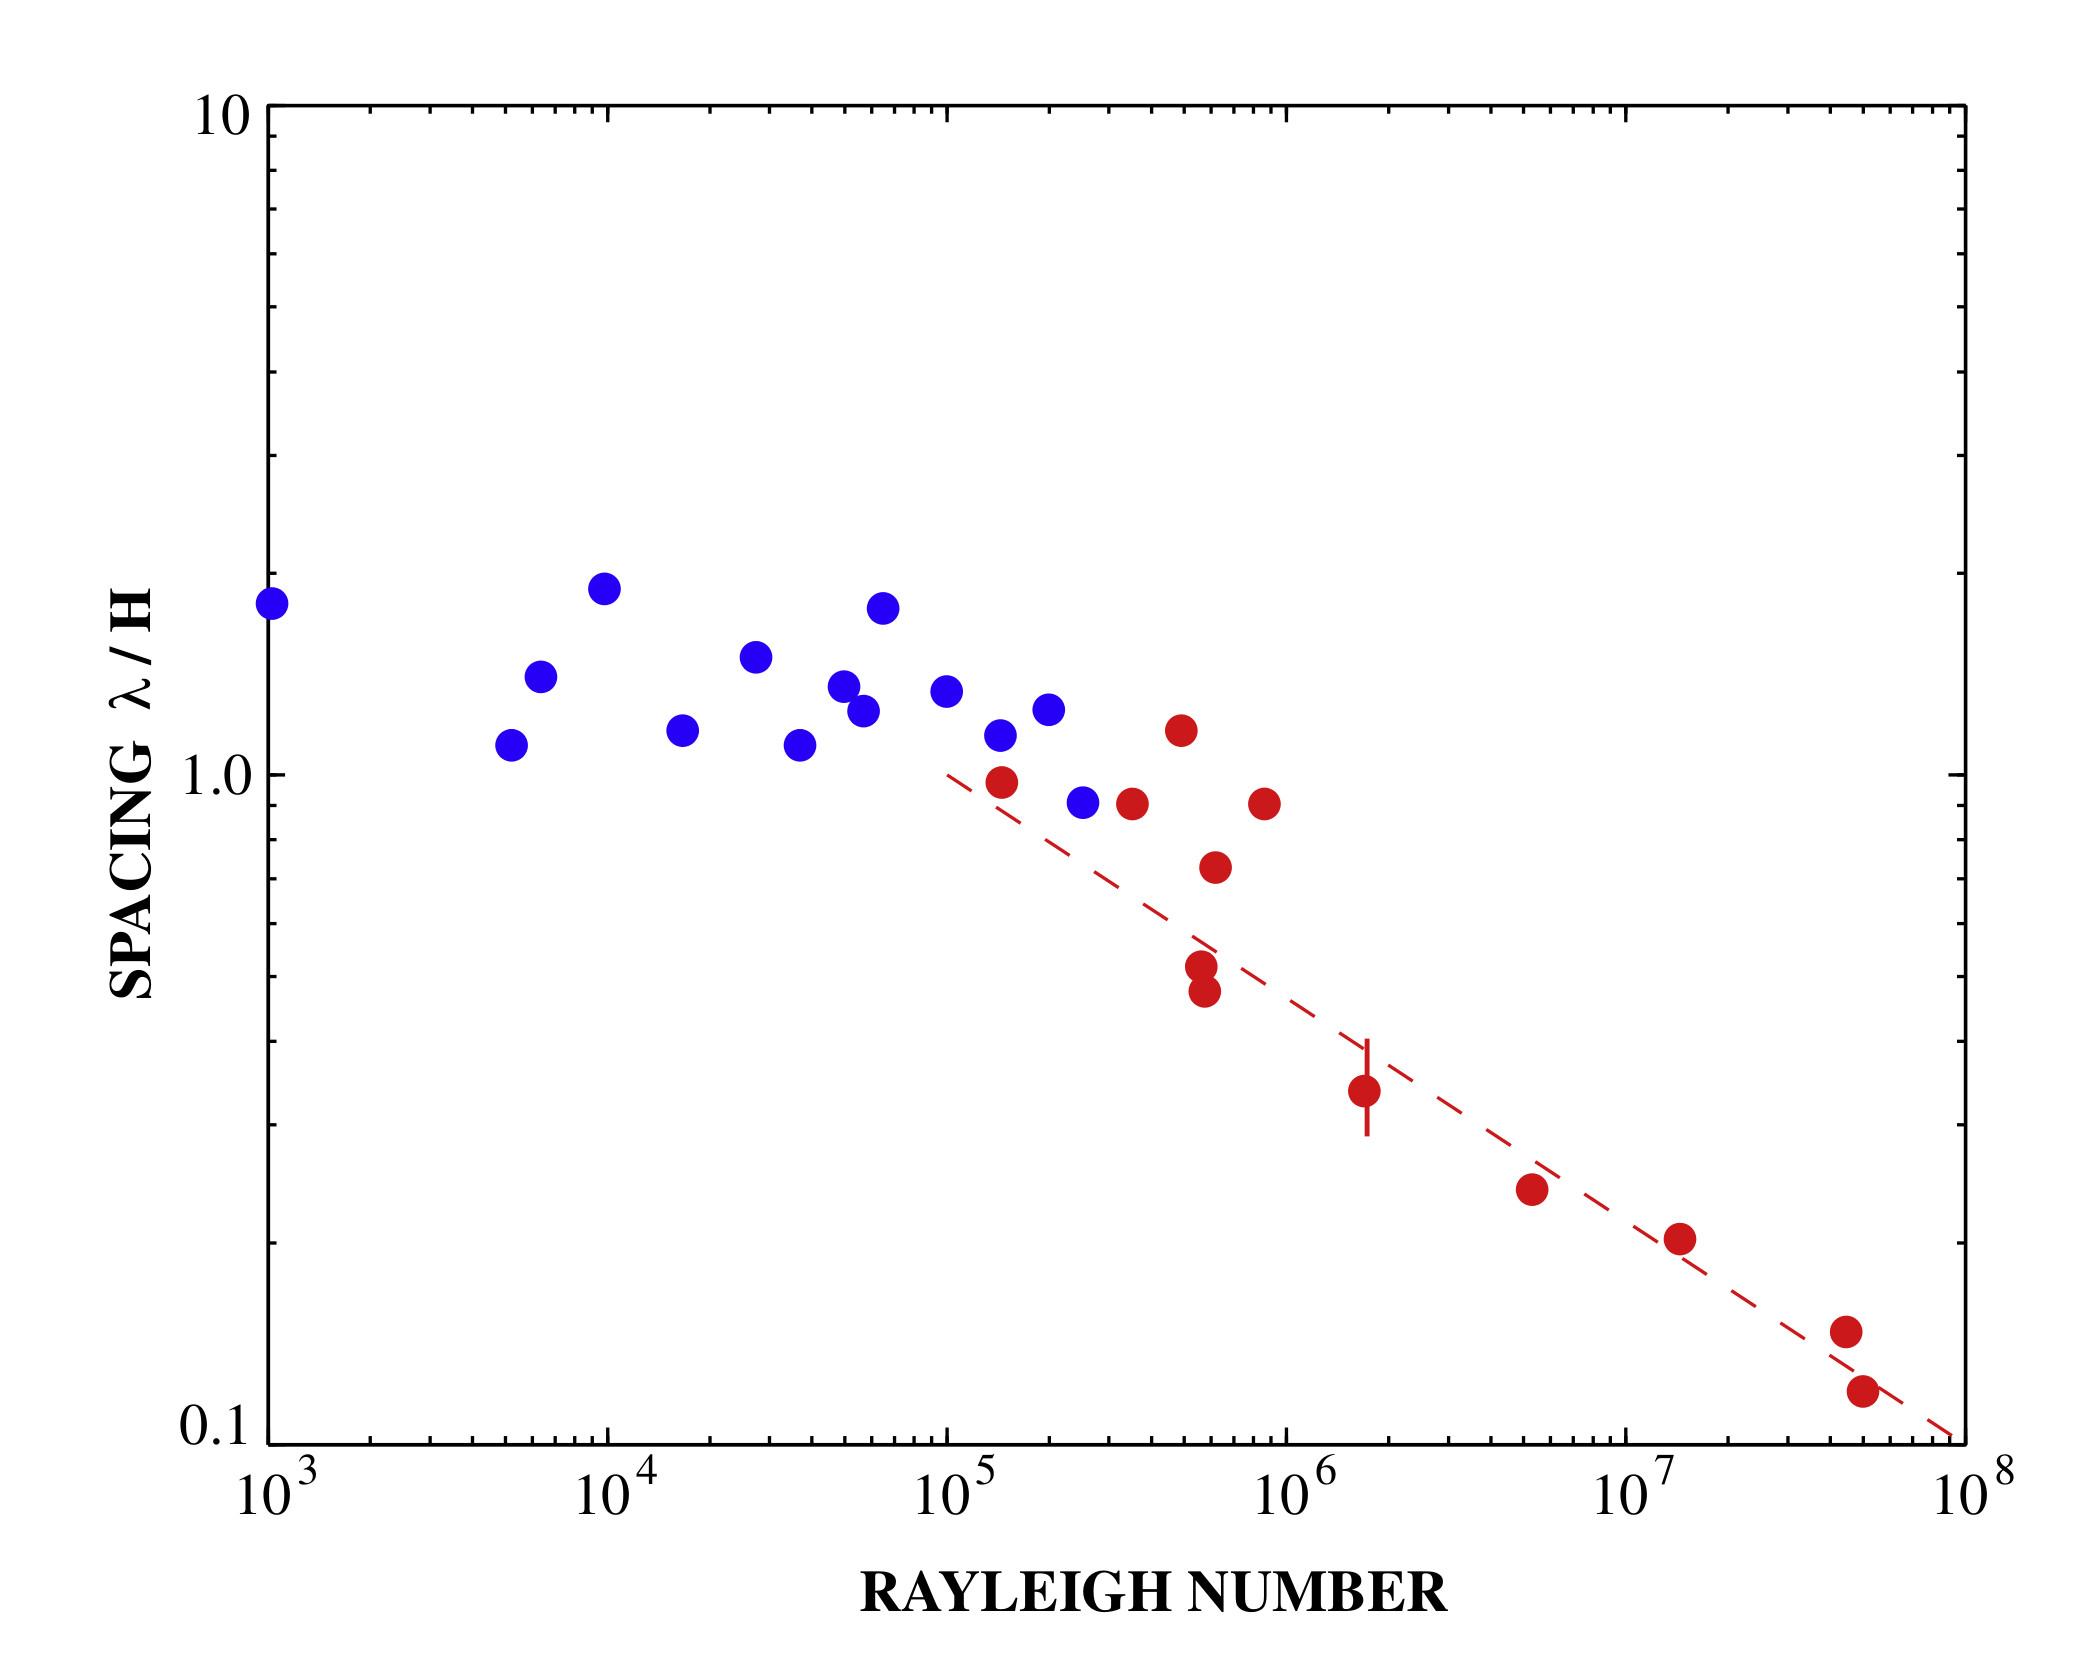
\includegraphics[height=0.7\paperheight]{./figures/androvandi-etal-pepi-2011.jpg}
        \caption{Laboratory experiments for temperature dependent viscosity suggests $\lambda \propto Ra^{-1/3}$ \citep{androvandi-etal-2011}.}
    \end{figure}
\end{frame}

\begin{frame}
    \frametitle{Relationship between Ra and $\lambda$}
    \begin{figure}
        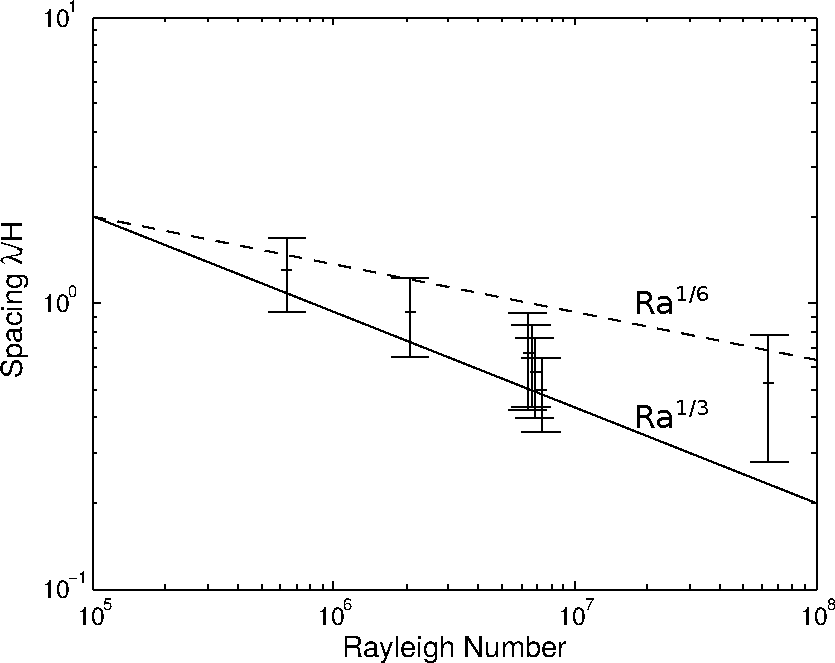
\includegraphics[height=0.7\paperheight]{./figures/RaWave-Stag3D.pdf}
        \caption{Numerical experiments for temperature dependent viscosity suggests $\lambda \propto Ra^{-1/3}$}
    \end{figure}
\end{frame}

\begin{frame}
    \frametitle{Conversion of instabilities to $V_{S}$}
    \begin{figure}
        \includegraphics[width=0.85\paperwidth]{./figures/Newt200/{dT1.1481_4x4_Newt_Ra6e6_7}.png}
        \caption{Thermal instabilities driven by a $200\rm\,^{\circ}C$ hot base. Newtonian rheology, $T_{P}=1350\rm\,^{\circ}C$; $Ra = 6\times10^{6}$.}
    \end{figure}
\end{frame}

\begin{frame}
\frametitle{Conversion of melt and temperature to $V_{S}$}
    \begin{itemize}
    \item[1]{Anharmonic effects: Use composition to map out mineral phases and calculate velocity using PerPleX \citep{connolly-2005}.}
    \item[2]{Melt effect: Assume strongest effect: -7.9\,\% drop in velocity per percent porosity, $\phi$, \citep{hammond-2000}.}
    \item[3]{Anelasticity: attenuation ($Q$) due to temperature ($T$) and dehydration {$C_{OH}$} due to melting, \\ $Q = A_{g}\left(\frac{C^{ref}_{OH}}{C_{OH}}\right)^{s}\omega^{\alpha} exp \left(\frac{\alpha\gamma T_{m}}{T} \right)$.}
    \item[4]{This gives a seismic shear-wave velocity ($V_{S}$), \\ $V_{S} = V_{\rm anh+melt} \left(1 - \frac{Q^{-1}}{2tan(\pi\alpha/2)}\right)$.}
    \end{itemize}
\end{frame}

\begin{frame}
    \frametitle{Conversion of instabilities to $V_{S}$}
    \begin{figure}
        %\vspace{-0.5cm}
        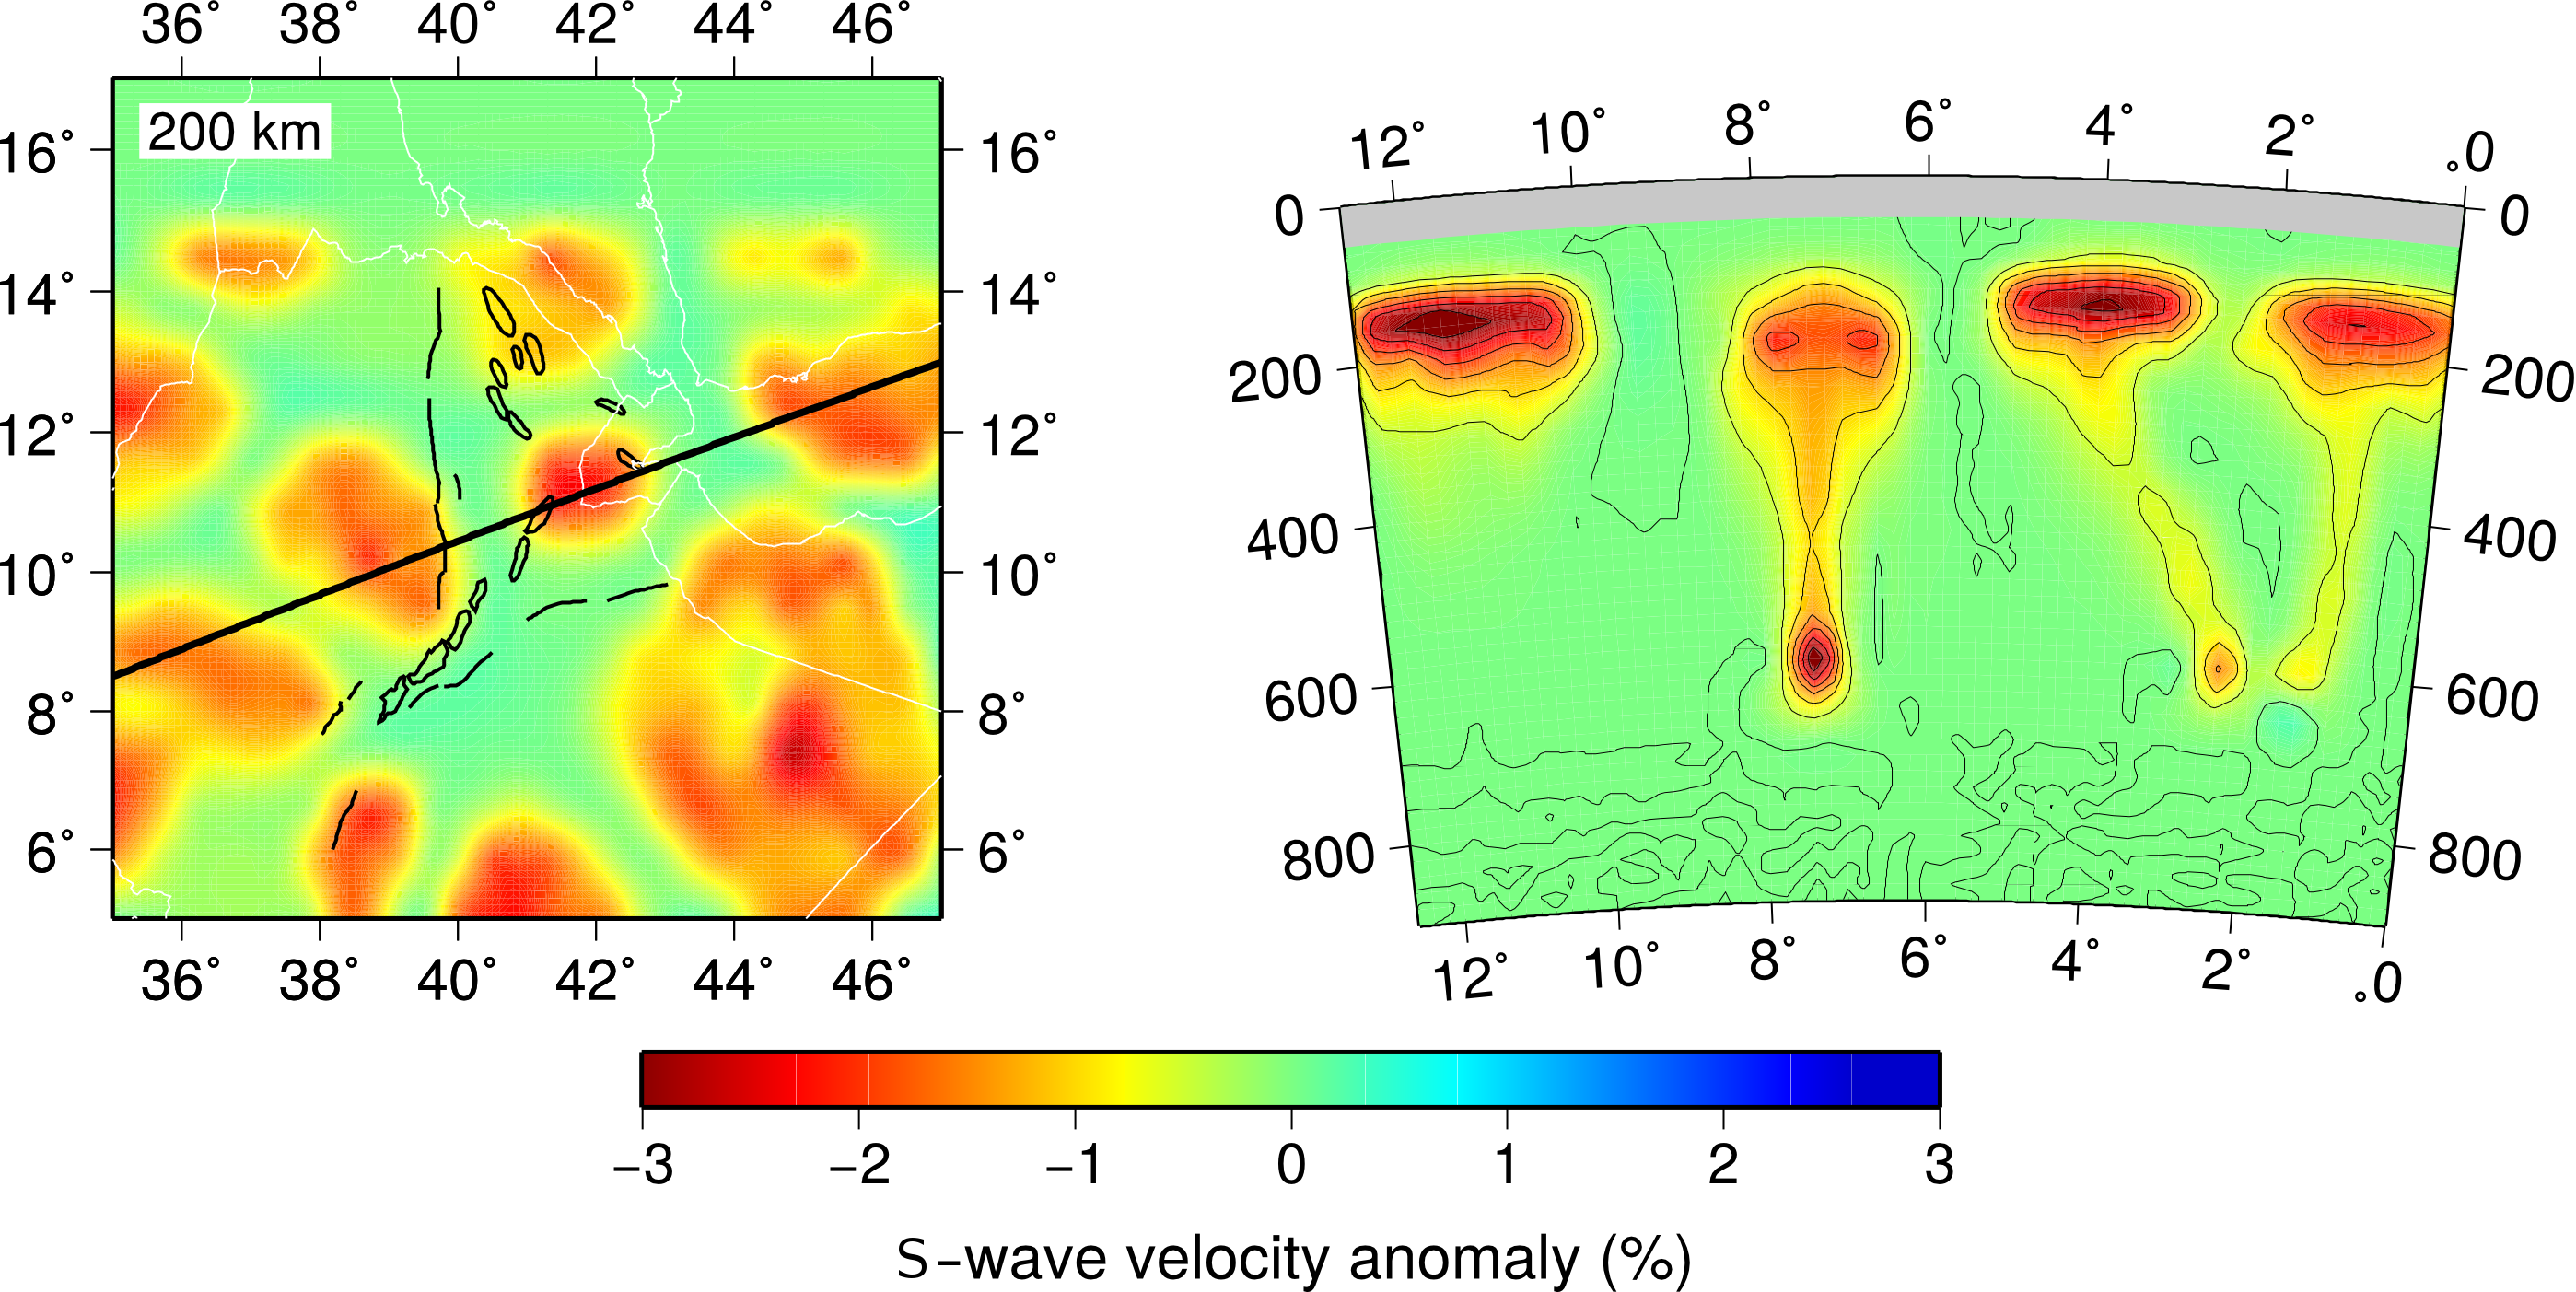
\includegraphics[width=0.85\paperwidth]{./figures/Newt200/input.png}
        \caption{Model seismic structure of Rayleigh B{\'e}nard convection}
    \end{figure}
\end{frame}

\begin{frame}
    \frametitle{Conversion of instabilities to synthetic tomography}
    \begin{figure}
        %\vspace{-0.5cm}
        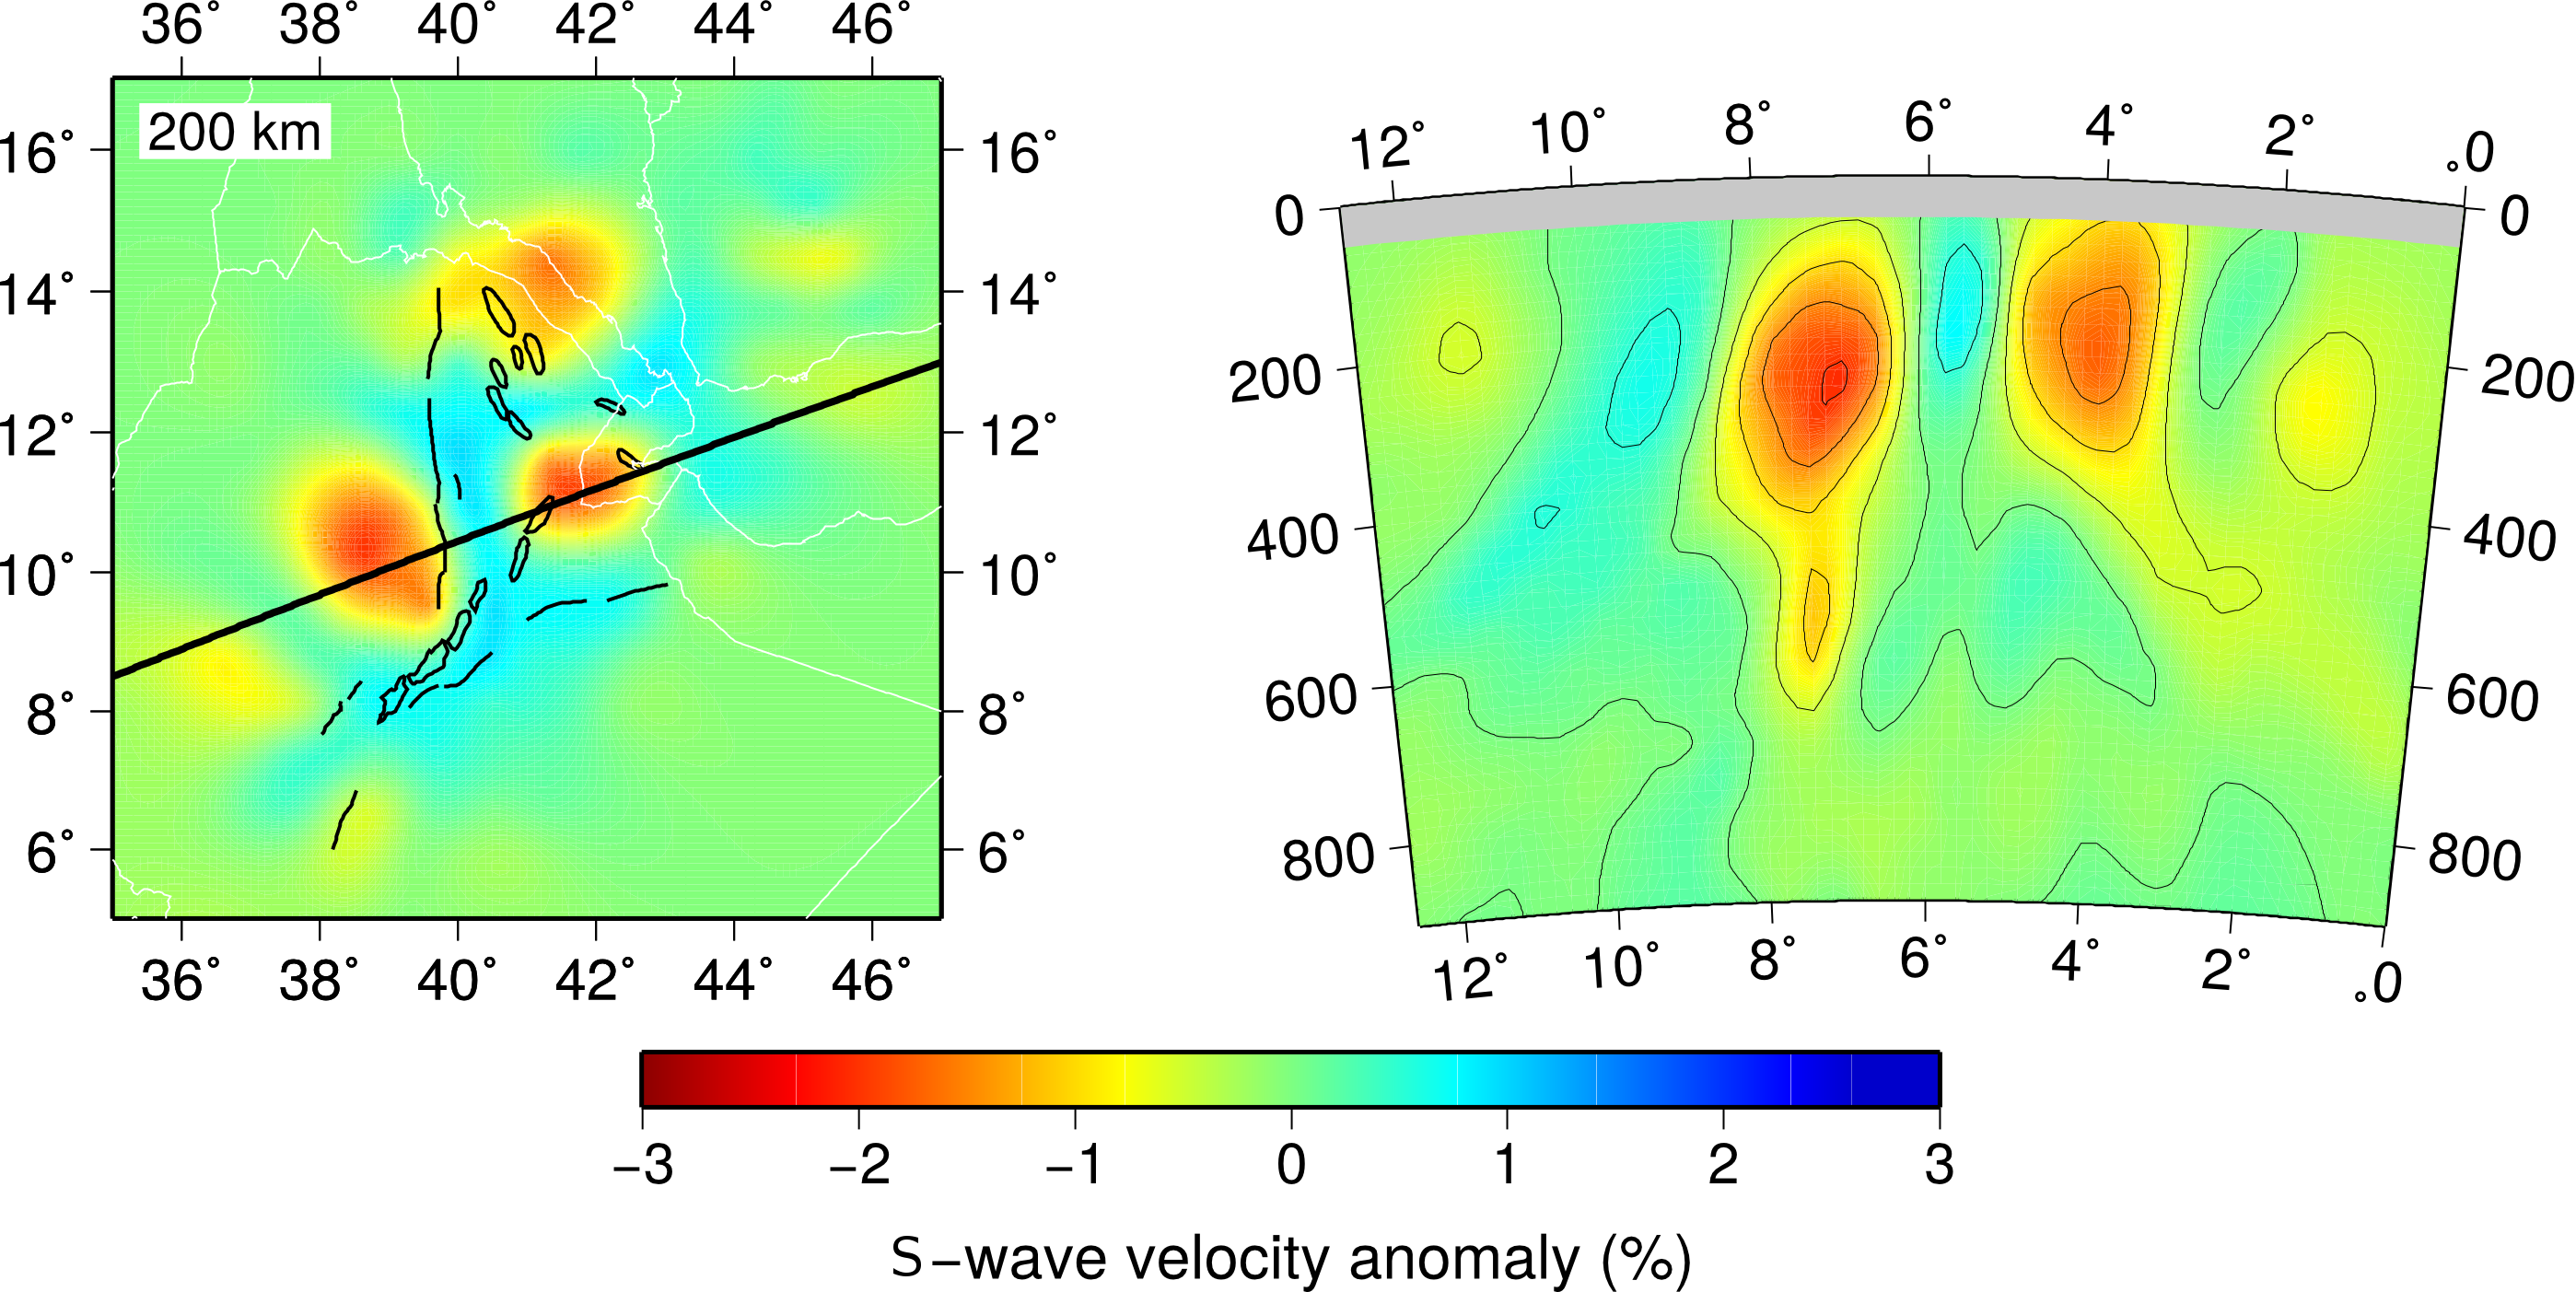
\includegraphics[width=0.85\paperwidth]{./figures/Newt200/output_damp.png}
        \caption{Rayleigh B{\'e}nard convection resolved by seismic array}
    \end{figure}
\end{frame}

\begin{frame}
    \frametitle{Comparison of synthetic tomography}
    \begin{figure}
        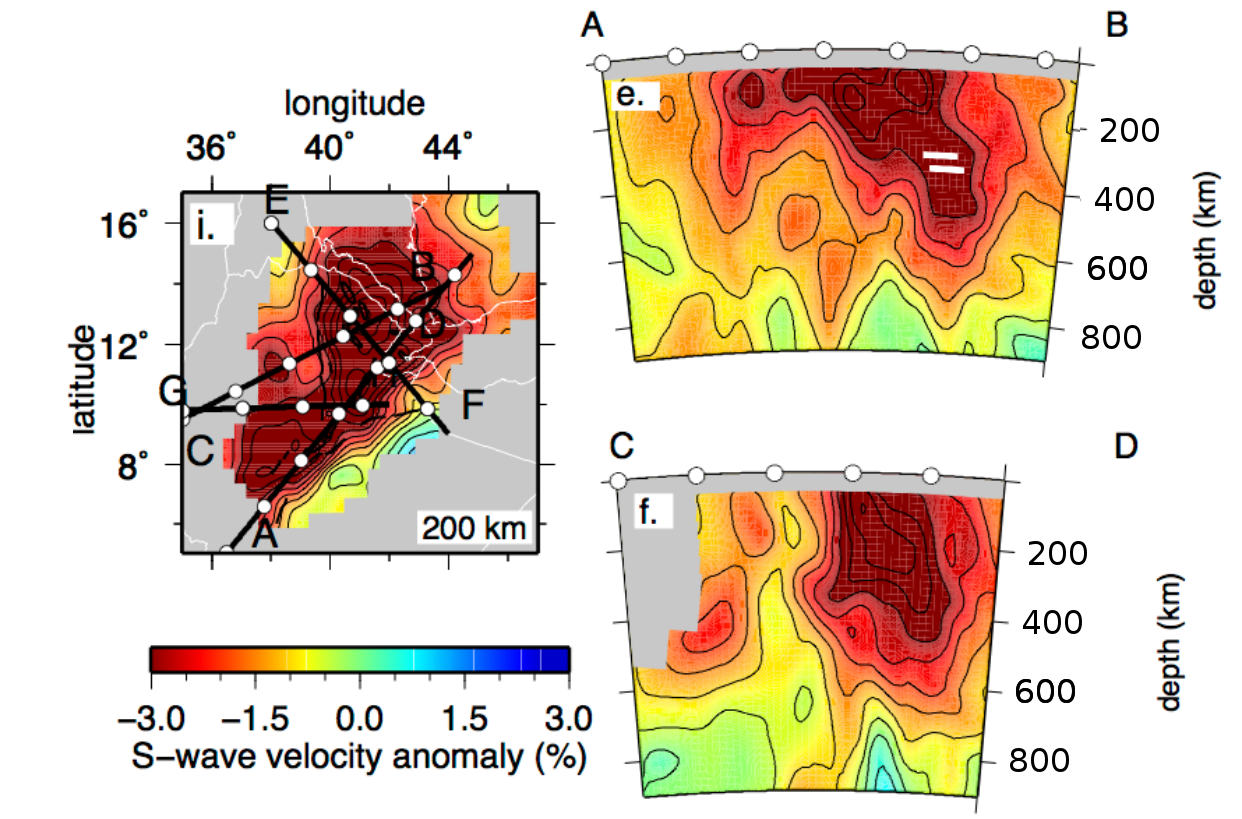
\includegraphics[height=0.7\paperheight]{./figures/chiara1.png}
        \caption{Rayleigh B{\'e}nard convection cannot create the gradient in velocity change that is seen in the inversion}
    \end{figure}
\end{frame}

\begin{frame}
    \frametitle{Secondary plumes or destabilisation?}
    \begin{figure}
        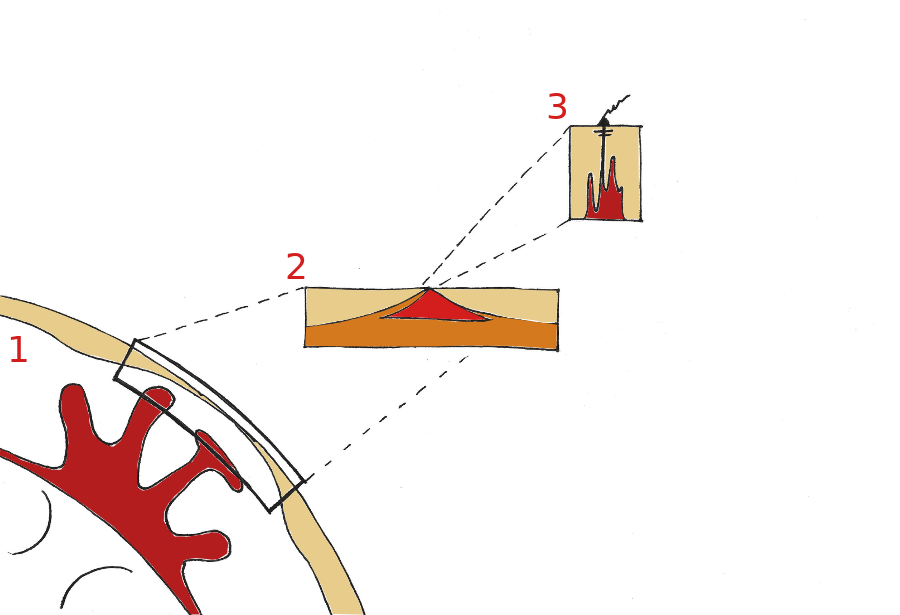
\includegraphics[height=0.9\paperheight]{./pictures/drawing.png}
    \end{figure}
\end{frame}

\begin{frame}
    \frametitle{Destabilisation of a hot layer}
    \begin{figure}
        \vspace{-.5cm}
        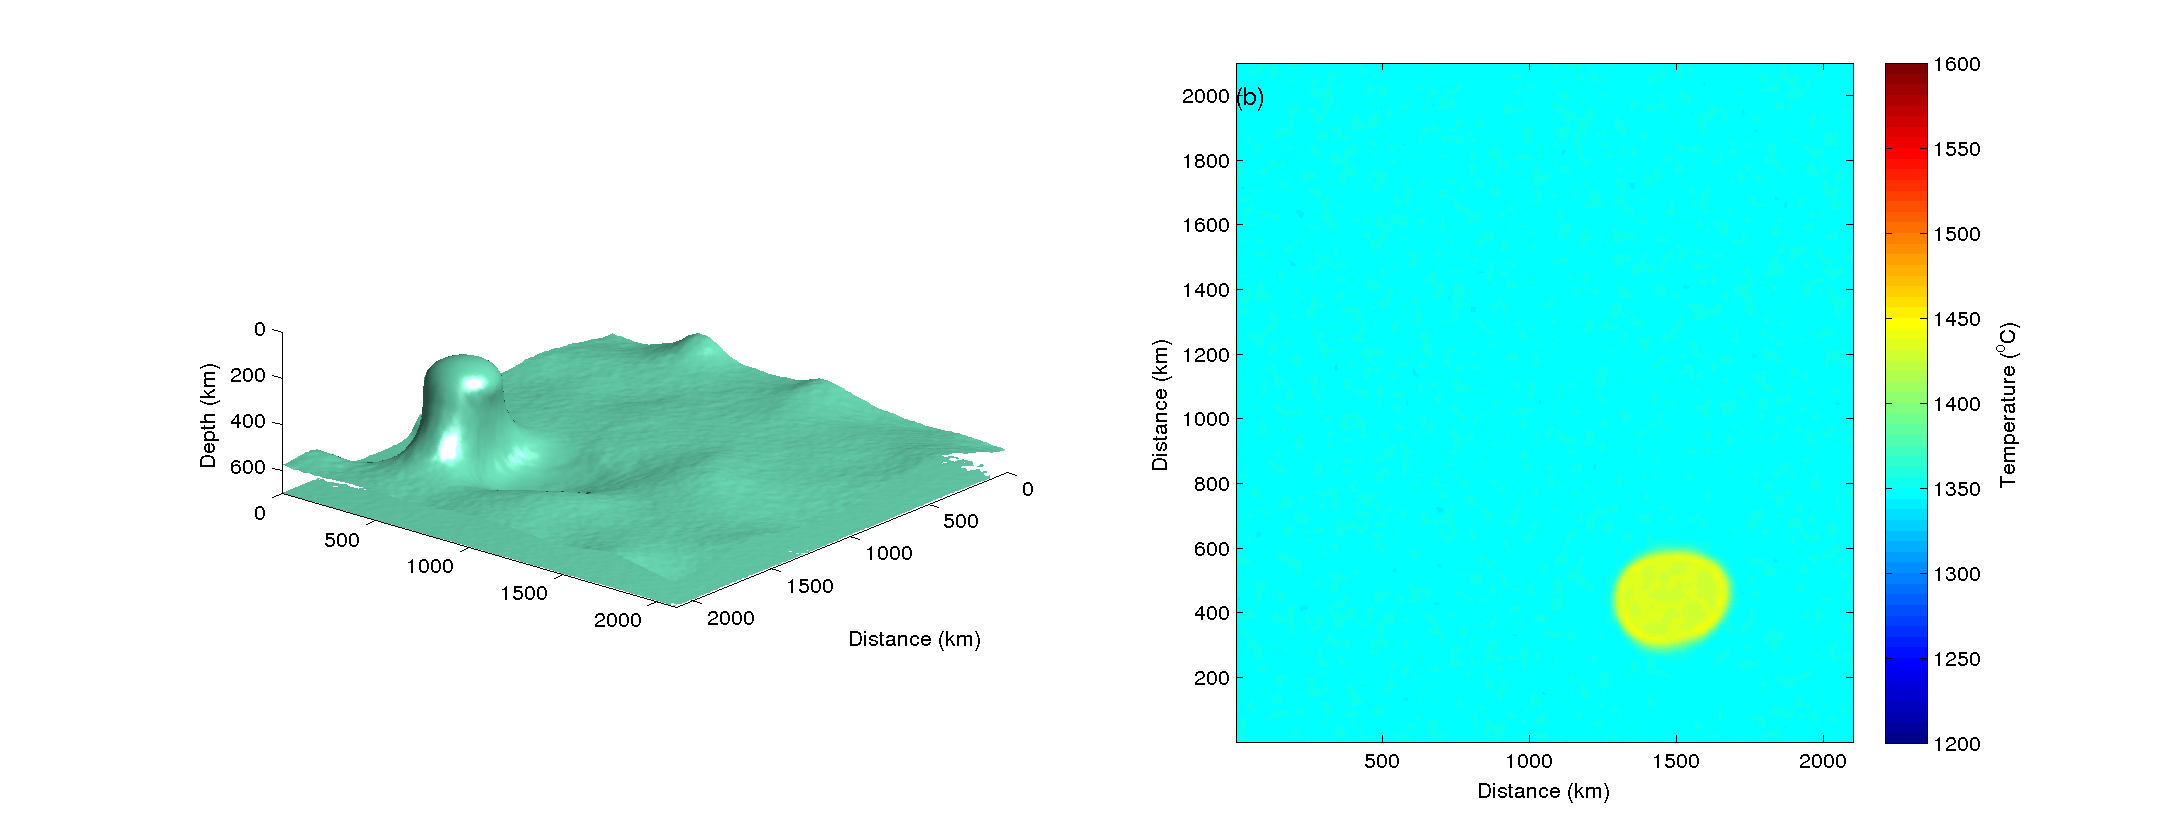
\includegraphics[width=0.85\paperwidth]{./figures/100hot/100hotbase_1.png}
        \caption{Destabilisation of a $100\rm\,^{\circ}C$ hot layer, non-Newtonian rheology, $T_{P}=1350\rm\,^{\circ}C$; $Ra = 6\times10^{6}$.}
    \end{figure}
\end{frame}

\begin{frame}
    \frametitle{Destabilisation of a hot layer}
    \begin{figure}
        \vspace{-.5cm}
        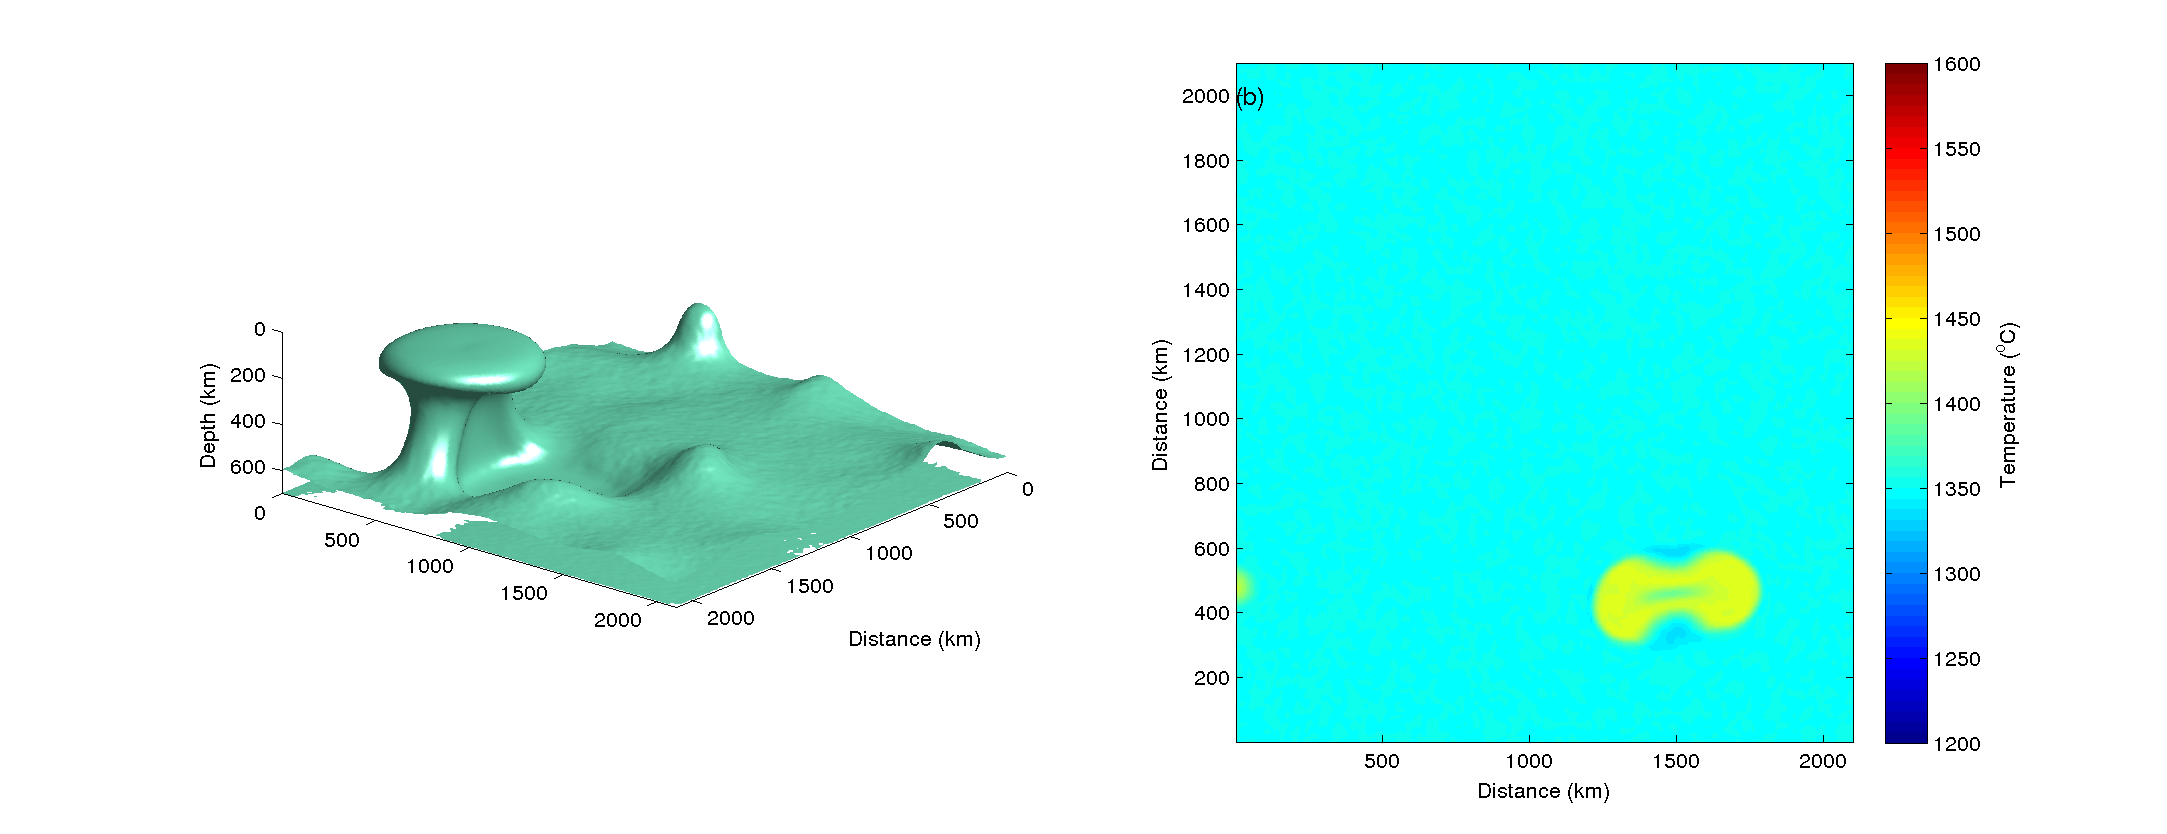
\includegraphics[width=0.85\paperwidth]{./figures/100hot/100hotbase_2.png}
        \caption{Destabilisation of a $100\rm\,^{\circ}C$ hot layer, non-Newtonian rheology, $T_{P}=1350\rm\,^{\circ}C$; $Ra = 6\times10^{6}$.}
    \end{figure}
\end{frame}

\begin{frame}
    \frametitle{Destabilisation of a hot layer}
    \begin{figure}
        \vspace{-.5cm}
        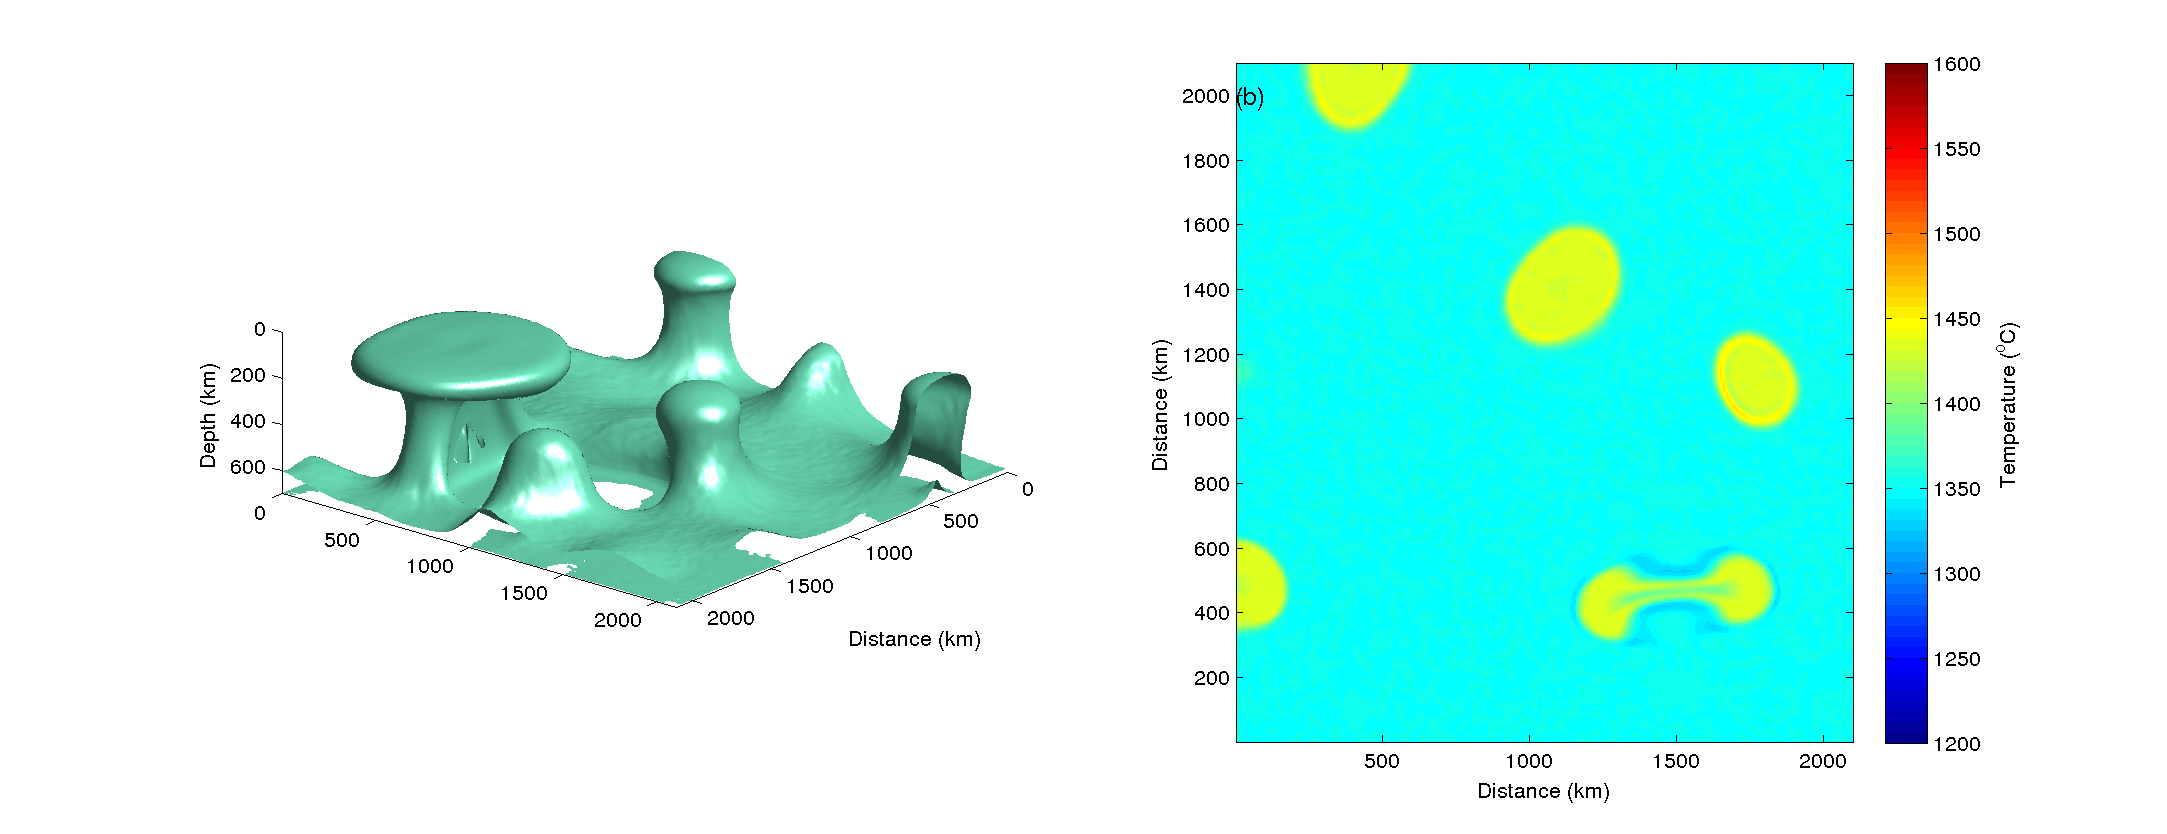
\includegraphics[width=0.85\paperwidth]{./figures/100hot/100hotbase_3.png}
        \caption{Destabilisation of a $100\rm\,^{\circ}C$ hot layer, non-Newtonian rheology, $T_{P}=1350\rm\,^{\circ}C$; $Ra = 6\times10^{6}$.}
    \end{figure}
\end{frame}

\begin{frame}
    \frametitle{Destabilisation of a hot layer}
    \begin{figure}
        \vspace{-.5cm}
        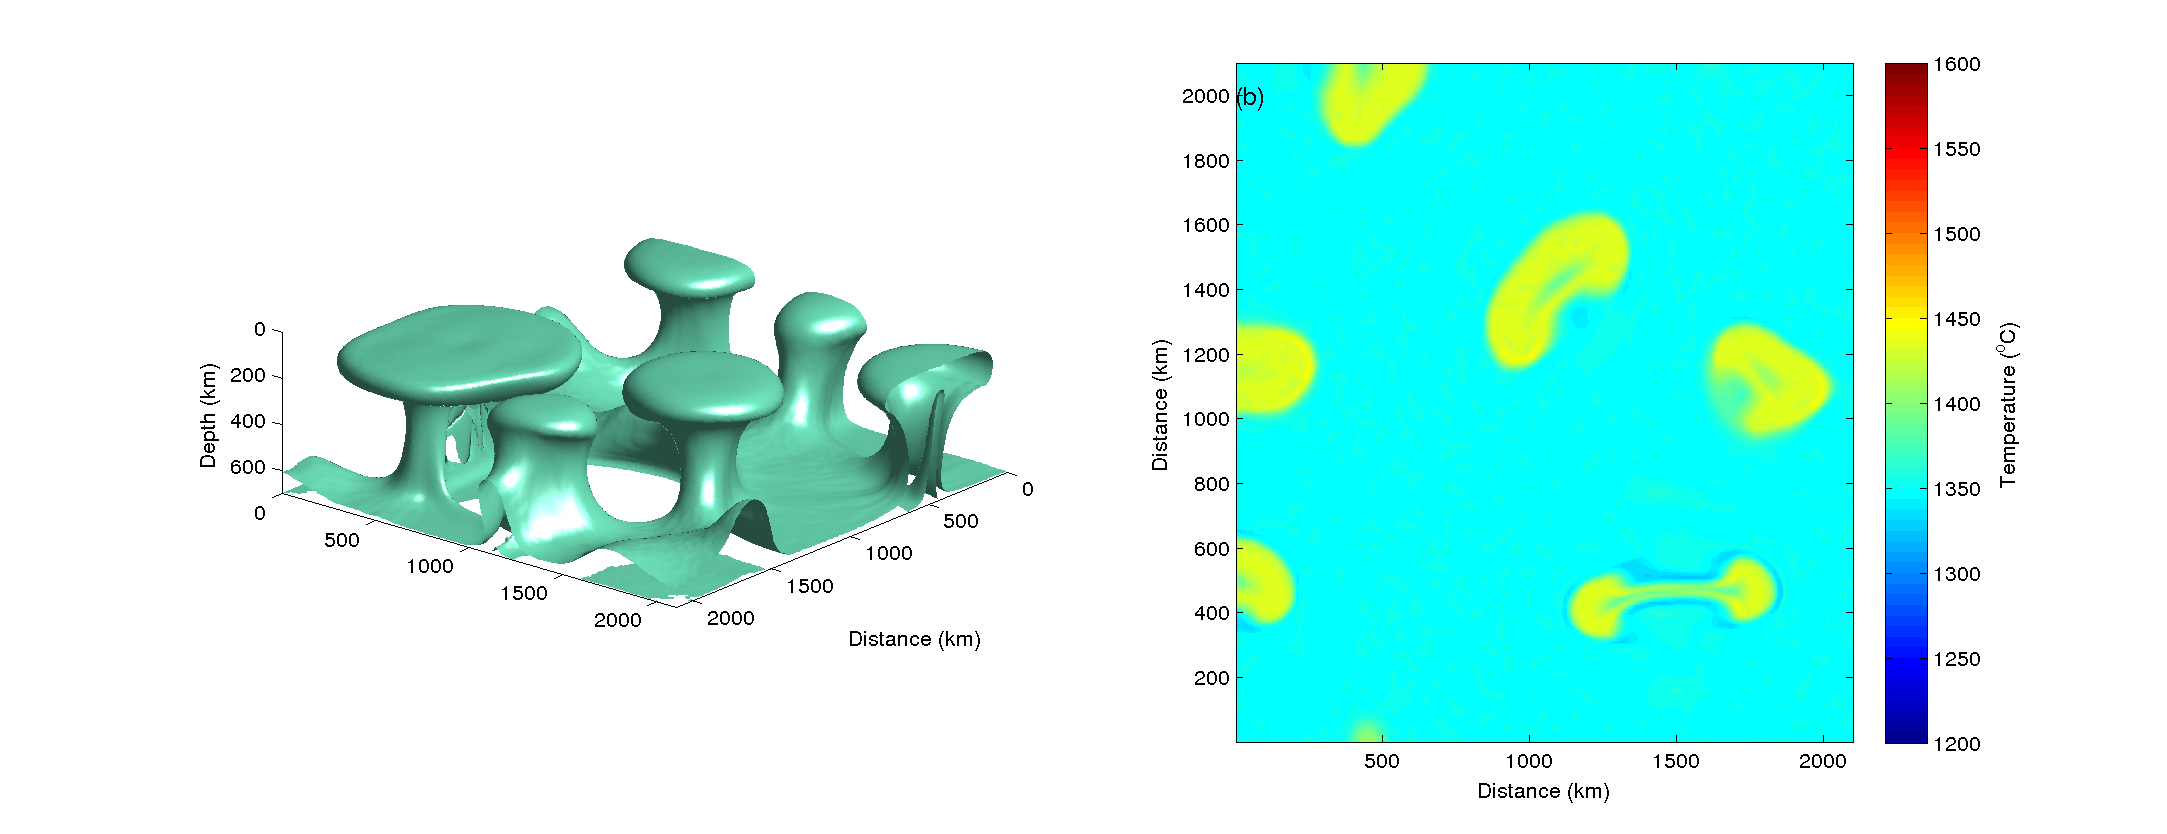
\includegraphics[width=0.85\paperwidth]{./figures/100hot/100hotbase_4.png}
        \caption{Destabilisation of a $100\rm\,^{\circ}C$ hot layer, non-Newtonian rheology, $T_{P}=1350\rm\,^{\circ}C$; $Ra = 6\times10^{6}$.}
    \end{figure}
\end{frame}

\begin{frame}
    \frametitle{Destabilisation of a hot layer}
    \begin{figure}
        \vspace{-.5cm}
        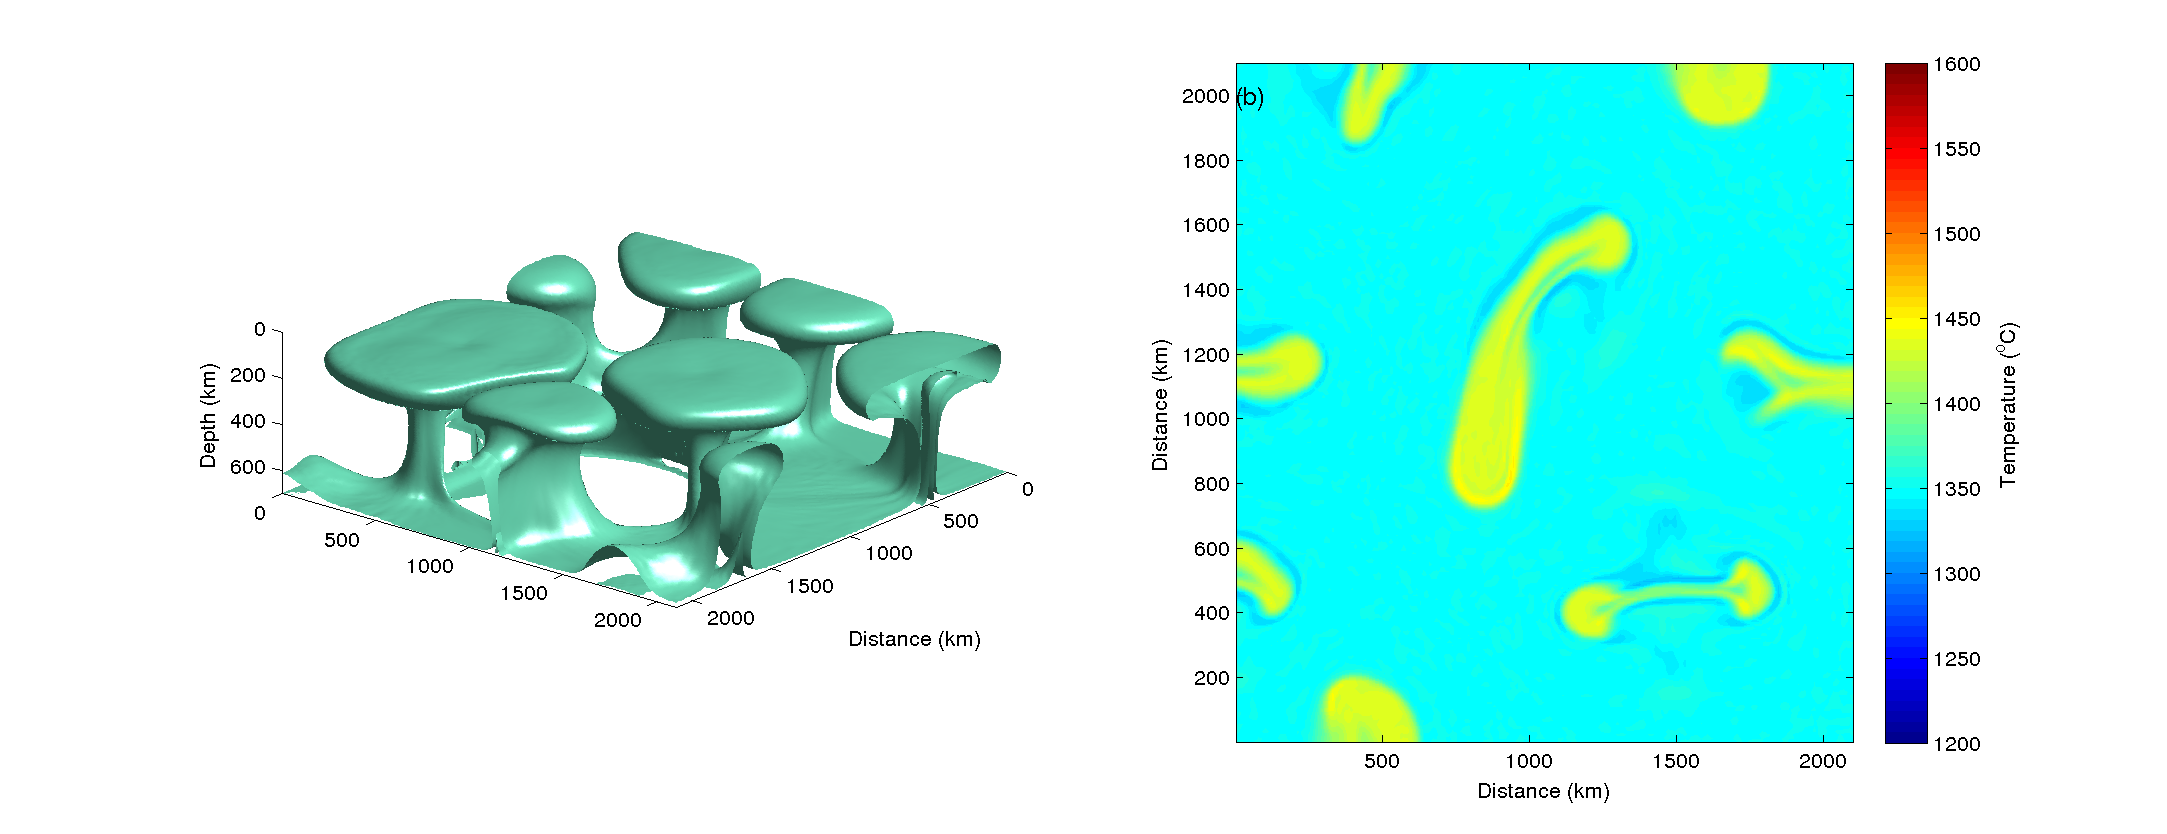
\includegraphics[width=0.85\paperwidth]{./figures/100hot/100hotbase_5.png}
        \caption{Destabilisation of a $100\rm\,^{\circ}C$ hot layer, non-Newtonian rheology, $T_{P}=1350\rm\,^{\circ}C$; $Ra = 6\times10^{6}$.}
    \end{figure}
\end{frame}

\begin{frame}
    \frametitle{Destabilisation of a hot layer}
    \begin{figure}
        \vspace{-.5cm}
        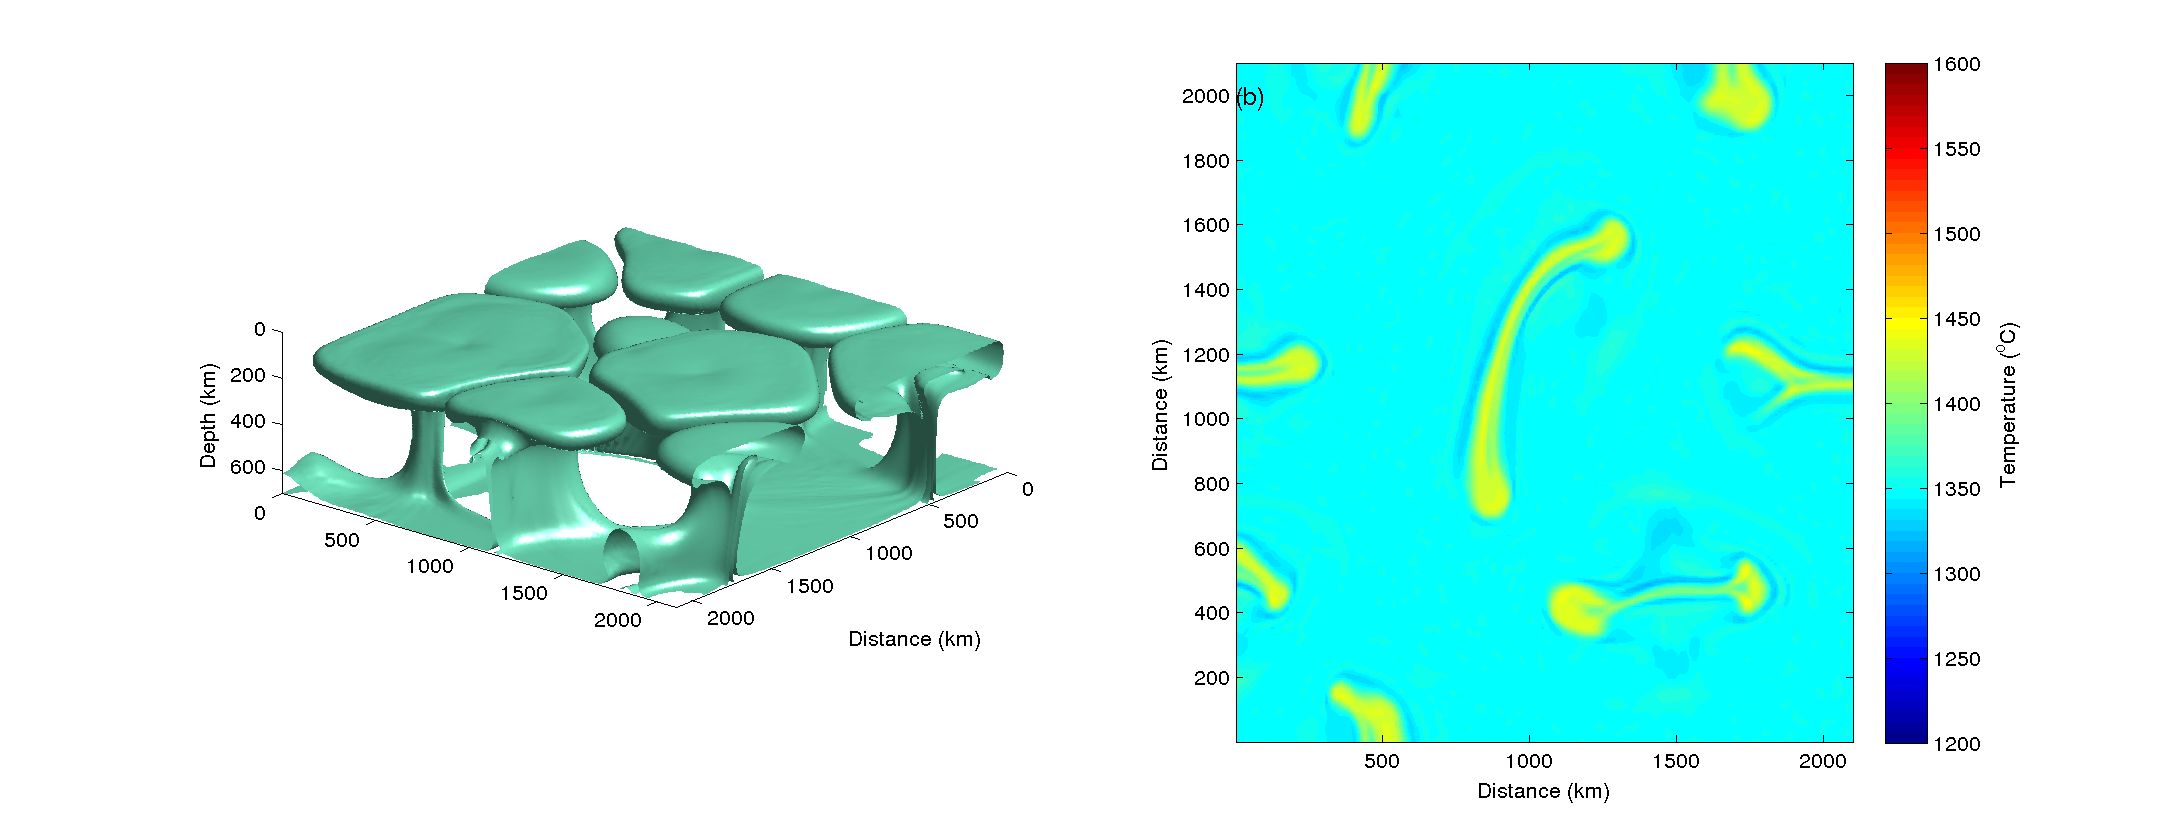
\includegraphics[width=0.85\paperwidth]{./figures/100hot/100hotbase_6.png}
        \caption{Destabilisation of a $100\rm\,^{\circ}C$ hot layer, non-Newtonian rheology, $T_{P}=1350\rm\,^{\circ}C$; $Ra = 6\times10^{6}$.}
    \end{figure}
\end{frame}

\begin{frame}
    \frametitle{Destabilisation of a hot layer}
    \begin{figure}
        \vspace{-.5cm}
        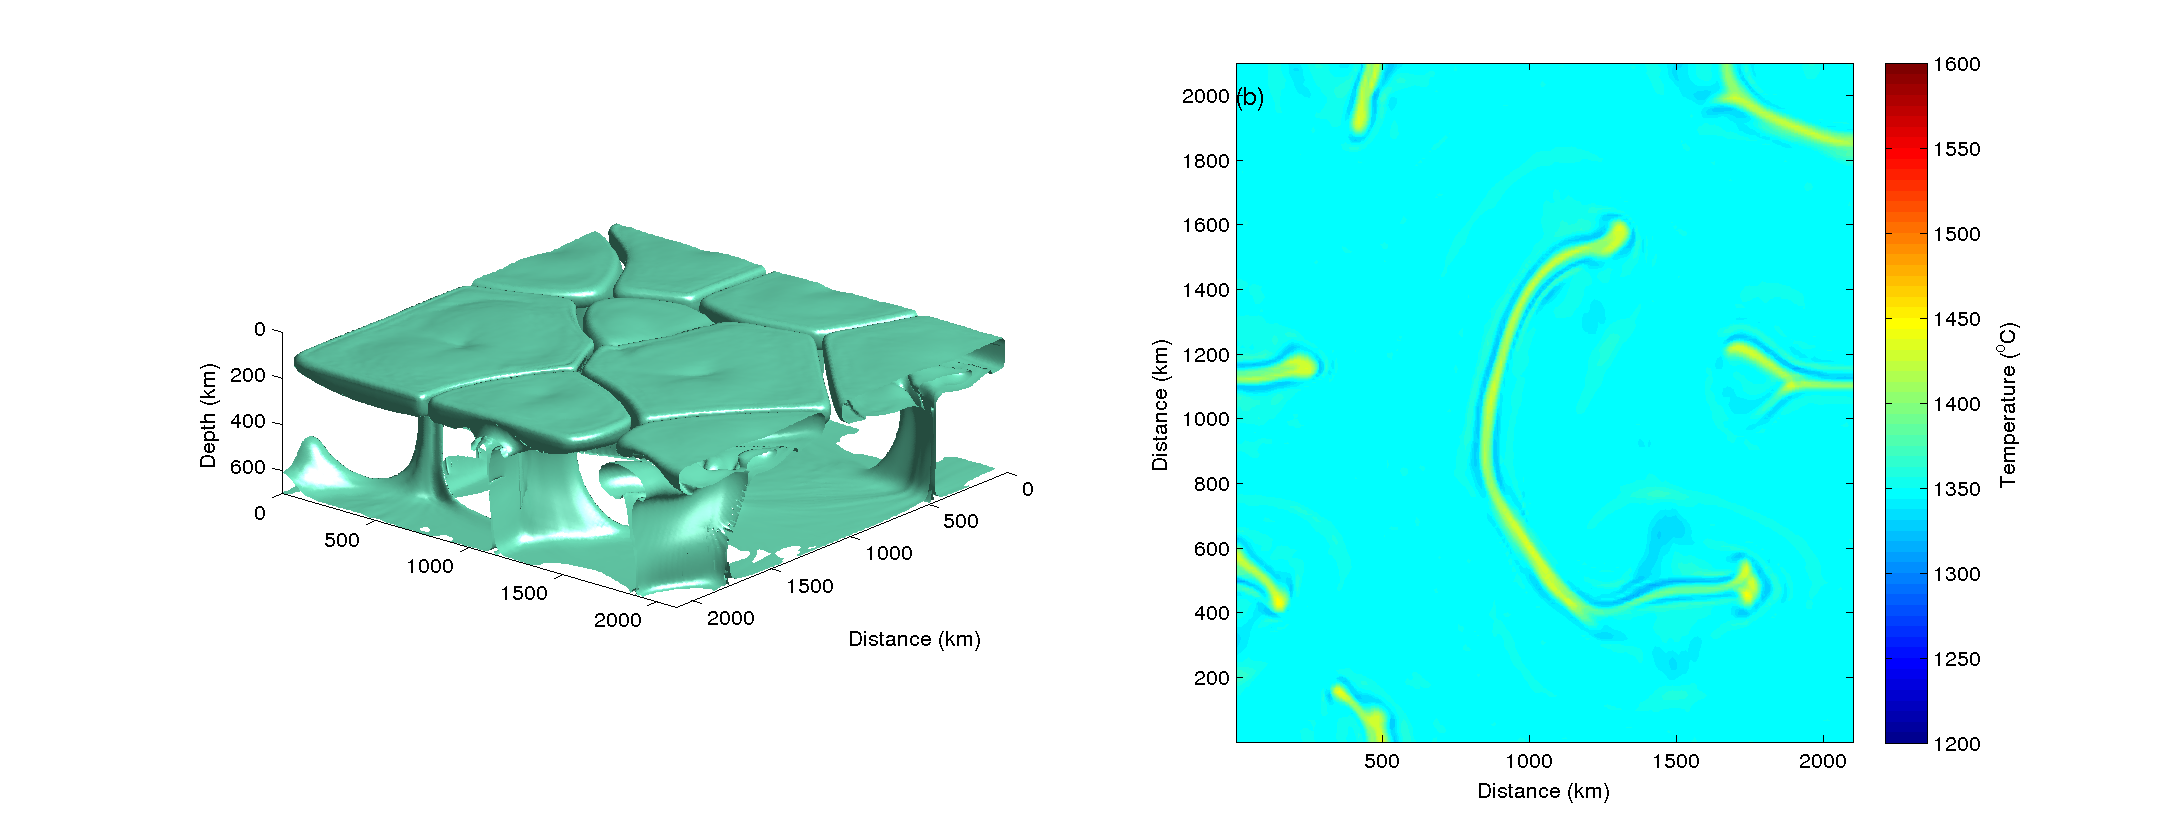
\includegraphics[width=0.85\paperwidth]{./figures/100hot/100hotbase_7.png}
        \caption{Destabilisation of a $100\rm\,^{\circ}C$ hot layer, non-Newtonian rheology, $T_{P}=1350\rm\,^{\circ}C$; $Ra = 6\times10^{6}$.}
    \end{figure}
\end{frame}

\begin{frame}
    \frametitle{Destabilisation of a hot layer: different stages of plume evolution}
    \begin{figure}
        \vspace{-.5cm}
        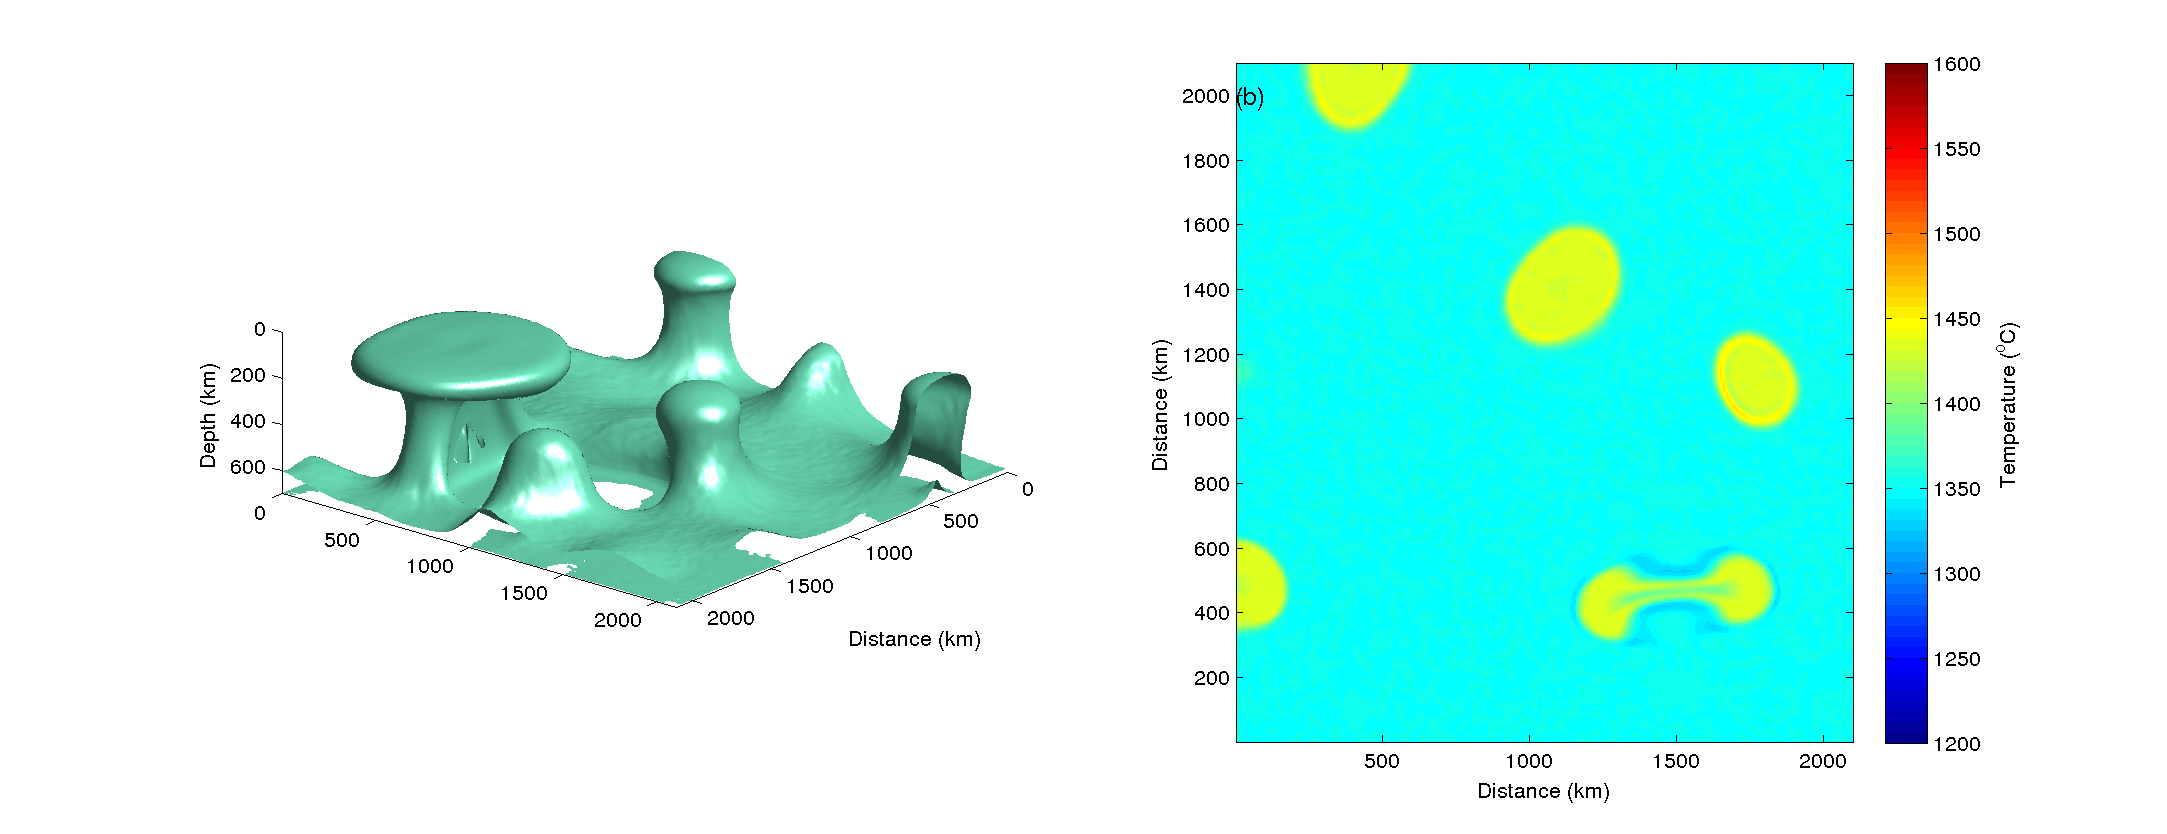
\includegraphics[width=0.85\paperwidth]{./figures/100hot/100hotbase_3.png}
        \caption{Destabilisation of a $100\rm\,^{\circ}C$ hot layer, non-Newtonian rheology, $T_{P}=1350\rm\,^{\circ}C$; $Ra = 6\times10^{6}$.}
    \end{figure}
\end{frame}

\begin{frame}
    \frametitle{Model - Tomography Comparison}
    \begin{figure}
        \vspace{-0.5cm}
        \includegraphics[width=0.85\paperwidth]{./figures/model-mer.png}
    \end{figure}
\end{frame}

\begin{frame}
    \frametitle{`Plumelets' below the Northern East African Rift}
    \begin{itemize}
    \item[-]{Despite trying everything the seismic inversion cannot be recreated by Rayleigh B{\'e}nard convection.}
        \SubItem{\textit{Plumelets have a temperature contrast that is too diffuse when resolved at the resolution of the seismic experiment.}}
        \SubItem{\textit{Plumelets with a non-Newtonian rheology have very thin tails that are invisible at the resolution of the seismic experiment.}}
    \item[-]{The destabilisation of a hot layer of mantle material best describes the tomographic model.}
        \SubItem{\textit{This however requires material to pond below the 660 discontinuity and then destabilise.}}
        \SubItem{\textit{Therefore the plumelets must be distinct from the background upper mantle.}}
    \item[-]{For more see \cite{civiero-etal-2020}. Work in collaboration with Chiara Civiero, Saskia Goes and James Hammond.}
    \end{itemize}
\end{frame}

\subsection{Melt generation}

\begin{frame}
    \frametitle{Part 1.2: Melt generation at zones of extension}
    \begin{figure}
        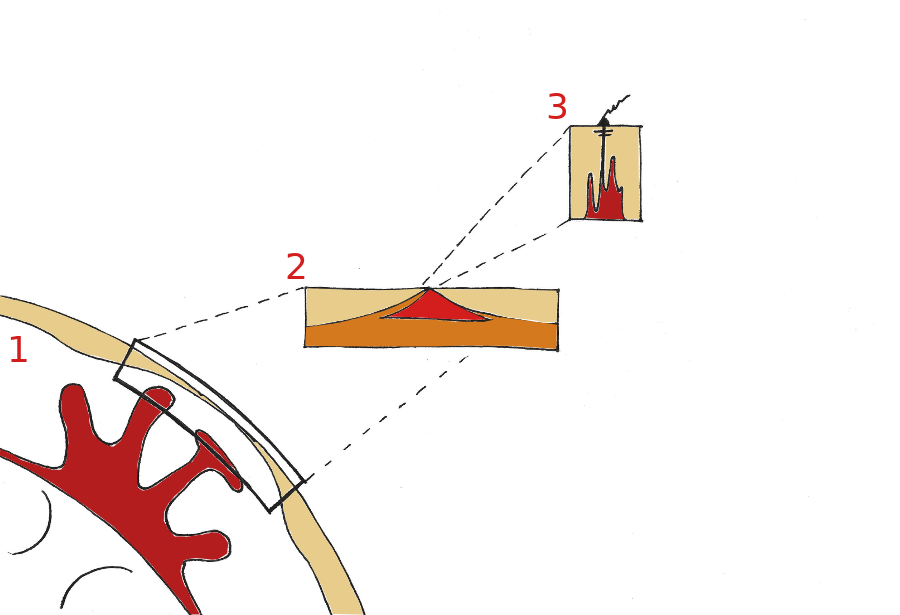
\includegraphics[height=0.9\paperheight]{./pictures/drawing.png}
    \end{figure}
\end{frame}

\begin{frame}
    \frametitle{Northern East African Rift}
    \begin{figure}
        \includegraphics[height=0.7\paperheight]{./figures/afar-crust-mantle.png}
        \caption{Narrow topographic expression of rifting in the southwest. Explained by focused localisation of stress or pre-existing weakness?}
    \end{figure}
\end{frame}

\begin{frame}
    \frametitle{Modelling decompression melting}
    \begin{itemize}
        \item[1]{Stokes flow and Boussinesq approximation}
        \item[2]{Decompression melt production ($\dot{m}$) and tracing of mantle composition ($C_{S}$),\\
                 $\dot{C_{S}} + {\bf V}_{S}.\nabla C_{S} = \left(1 - \frac{1}{D}\right)\frac{C_{S}}{\rho(1-\phi)}\dot{m}$}.
        \item[3]{Solve in a 2D domain with extension applied as a kinematic boundary condition that deforms the domain.}
        \item[4]{Model developed with Kenni Petersen}
    \end{itemize}
\end{frame}

\begin{frame}
    \frametitle{Visoc-elasto-plastic model with melting}
    \begin{figure}
        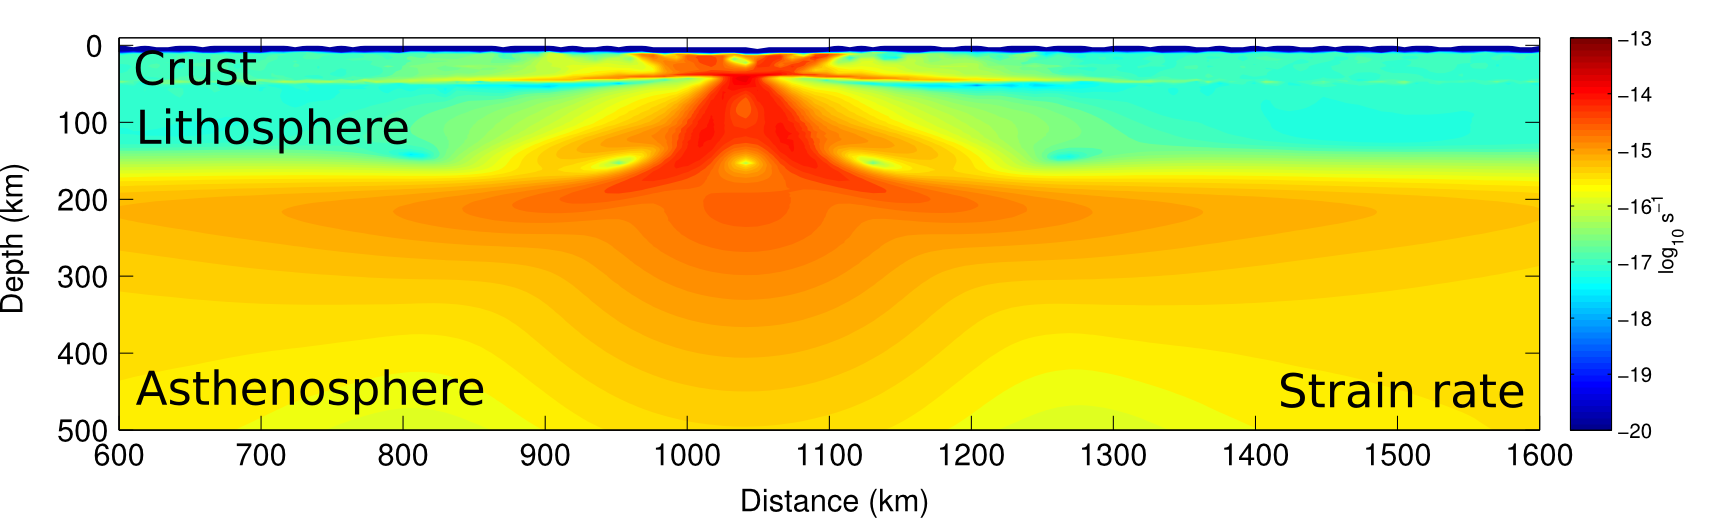
\includegraphics[width=0.8\paperwidth]{./figures/mess-example.png}
        \caption{Example of stress field during extension which can be driven by force or velocity boundary conditions}
    \end{figure}
\end{frame}

\begin{frame}
    \frametitle{Visoc-elasto-plastic model with melting}
    \begin{figure}
        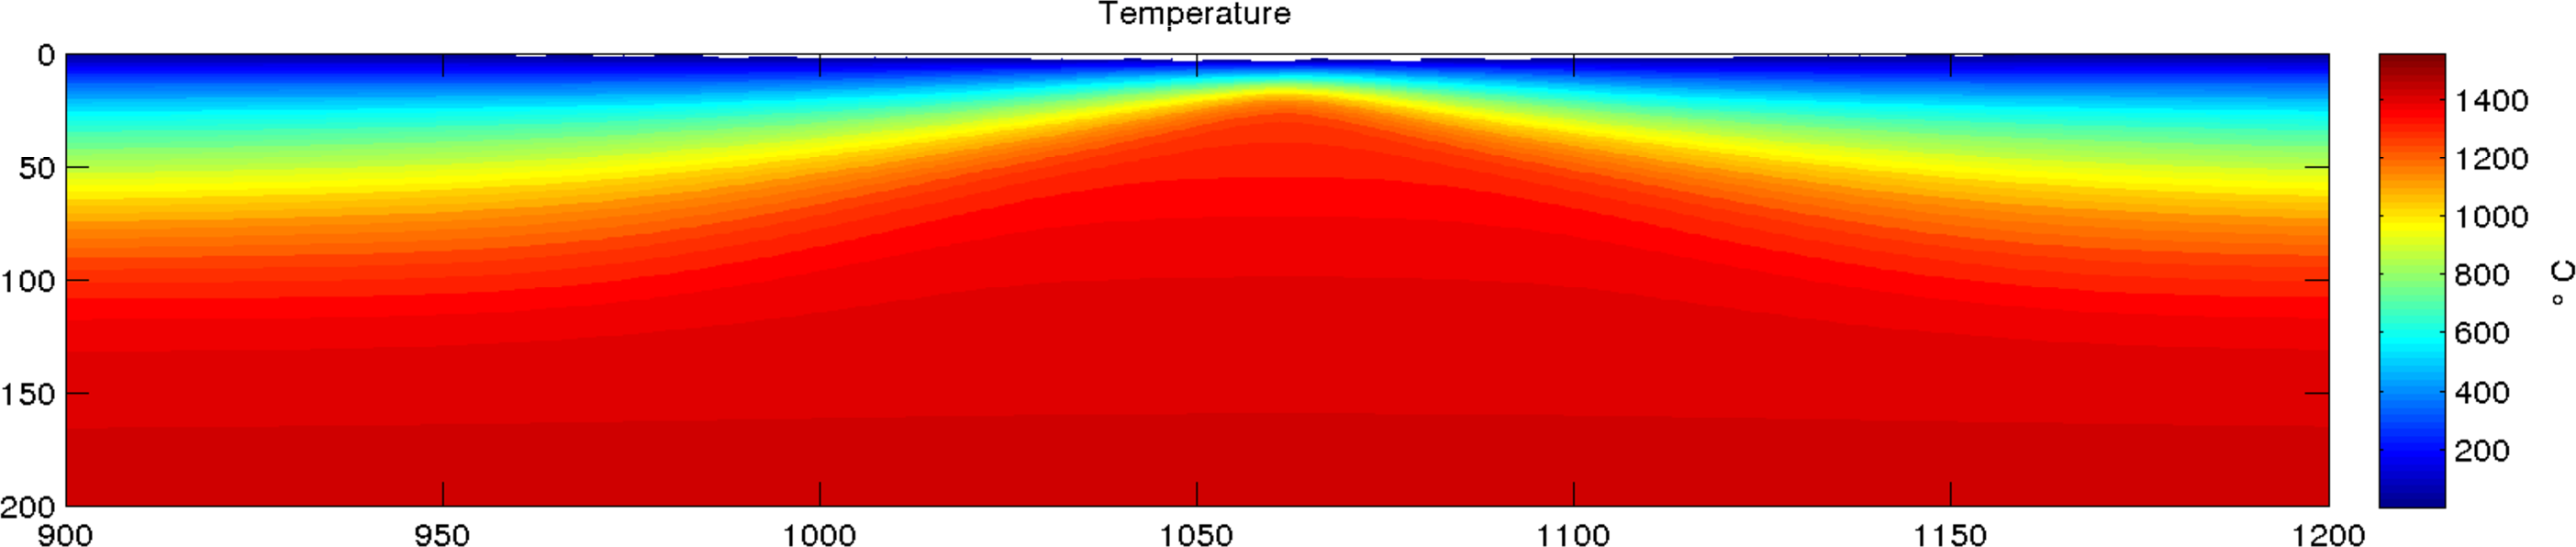
\includegraphics[width=0.8\paperwidth]{./figures/MESS1.png}
        \caption{Extension at $5\rm\,mm\,yr^{-1}$ for 25\,Myr with a mantle potential temperature of $1350\,^{\circ}\rm C$}
    \end{figure}
\end{frame}

\begin{frame}
    \frametitle{Visoc-elasto-plastic model with melting}
    \begin{figure}
        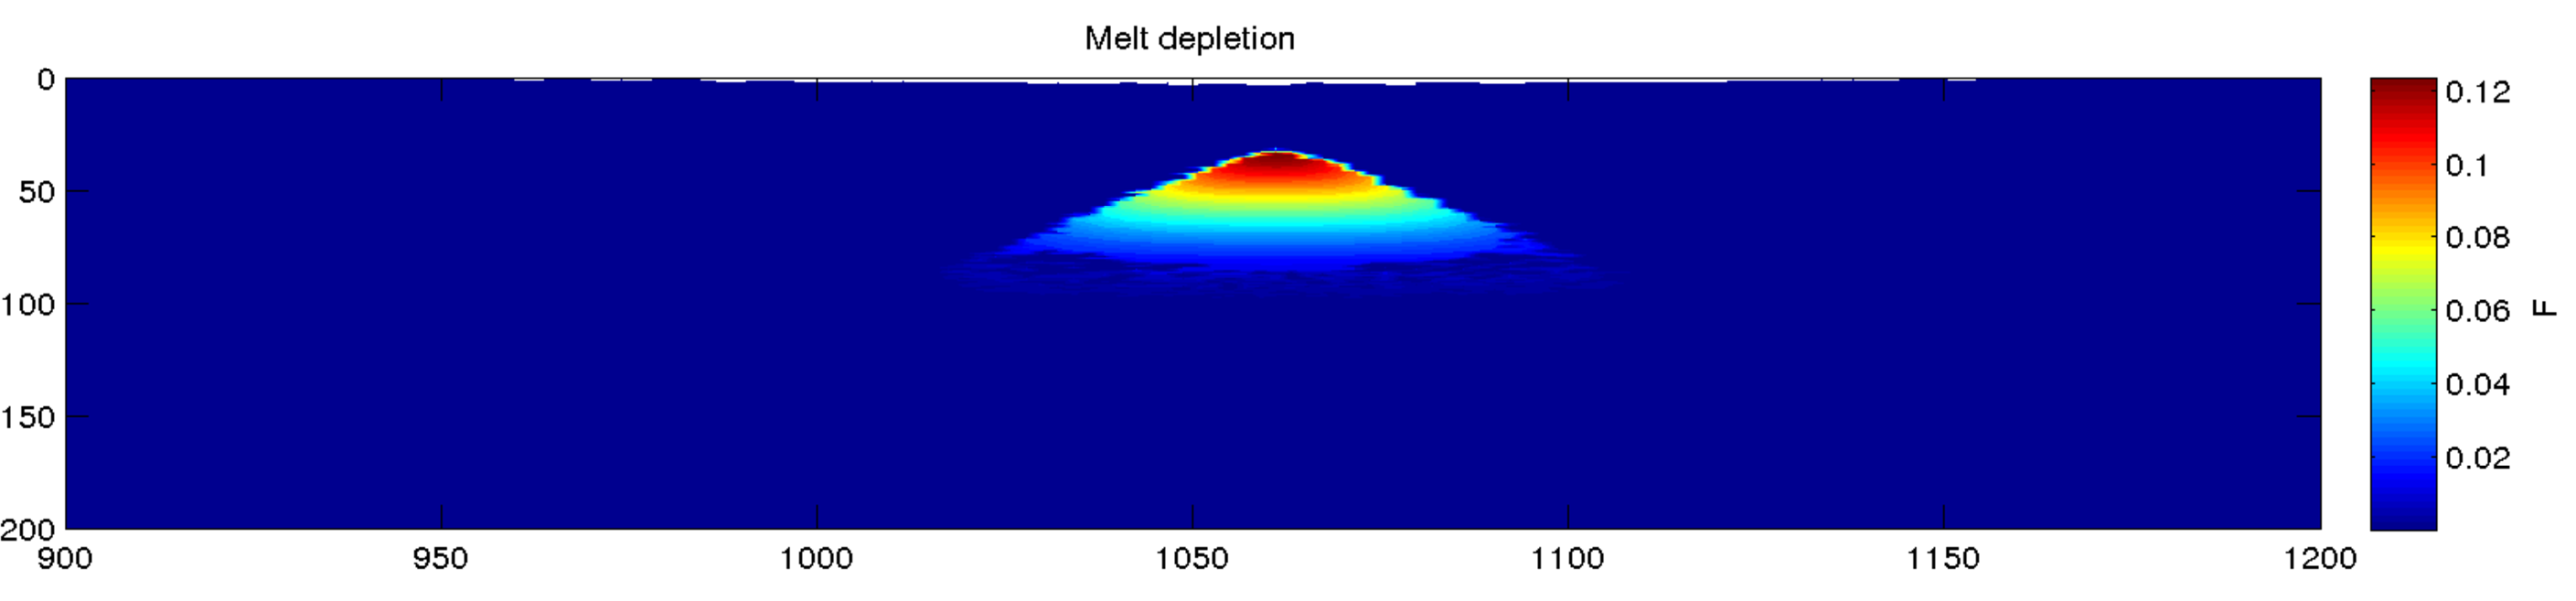
\includegraphics[width=0.8\paperwidth]{./figures/MESS2.png}
        \caption{Melt depletion at $5\rm\,mm\,yr^{-1}$ for 25\,Myr with a mantle potential temperature of $1350\,^{\circ}\rm C$}
    \end{figure}
\end{frame}

\begin{frame}
    \frametitle{Visoc-elasto-plastic model to seismic structure}
    \begin{figure}
        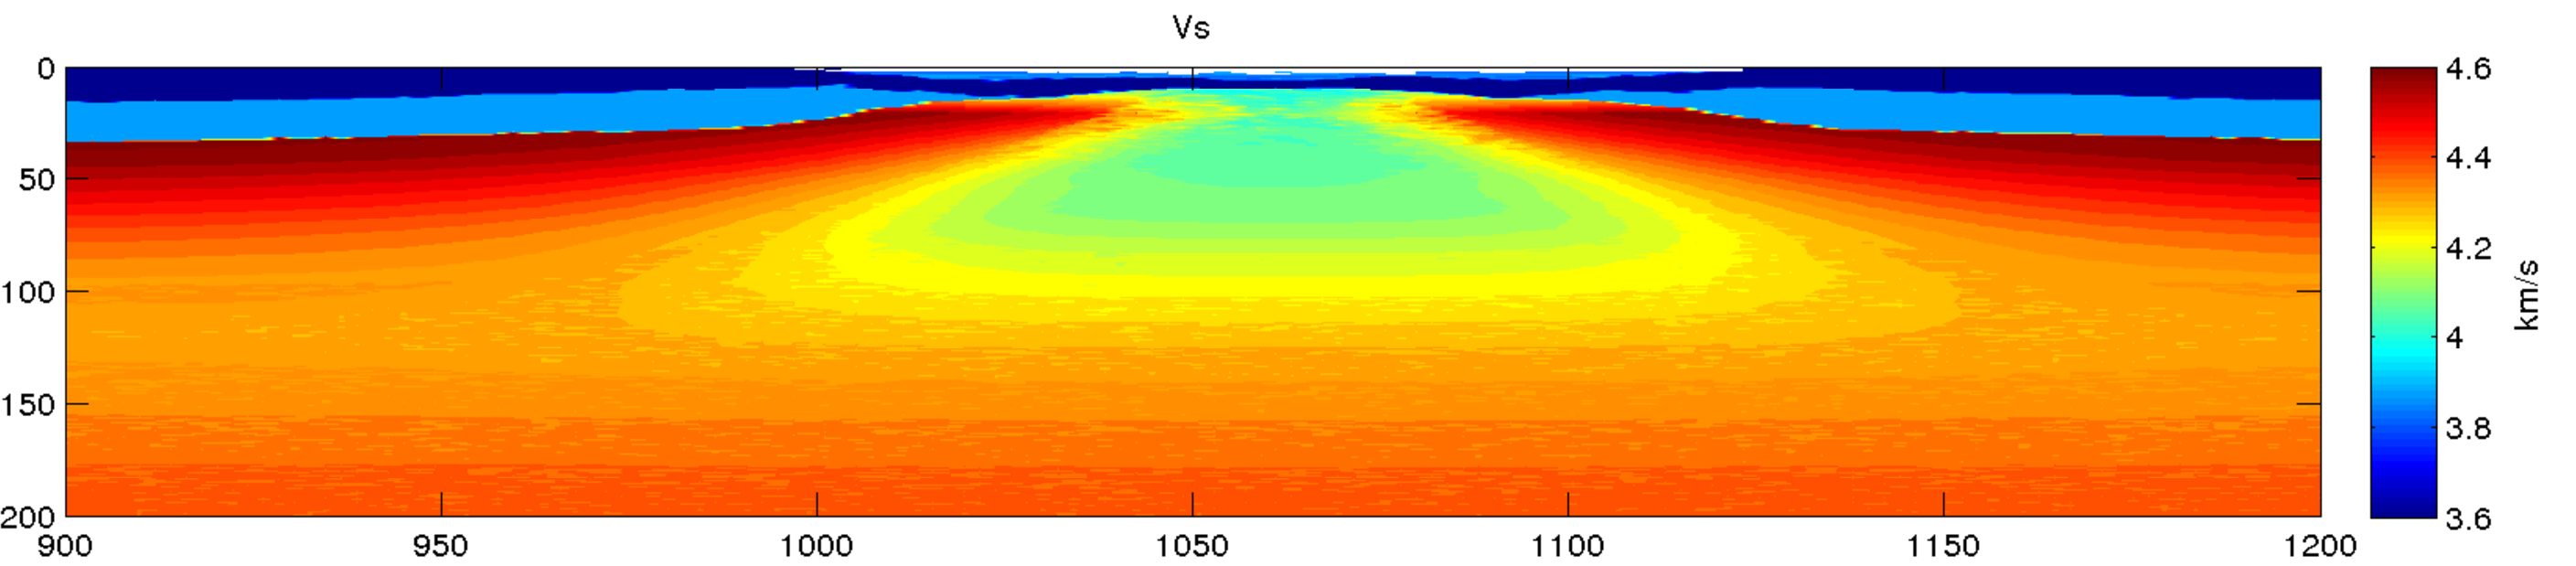
\includegraphics[width=0.8\paperwidth]{./figures/MER1.png}
        \caption{Seismic velocity at $5\rm\,mm\,yr^{-1}$ for 25\,Myr with a mantle potential temperature of $1350\,^{\circ}\rm C$}
    \end{figure}
\end{frame}

\begin{frame}
    \frametitle{Visoc-elasto-plastic model to seismic structure}
    \begin{figure}
        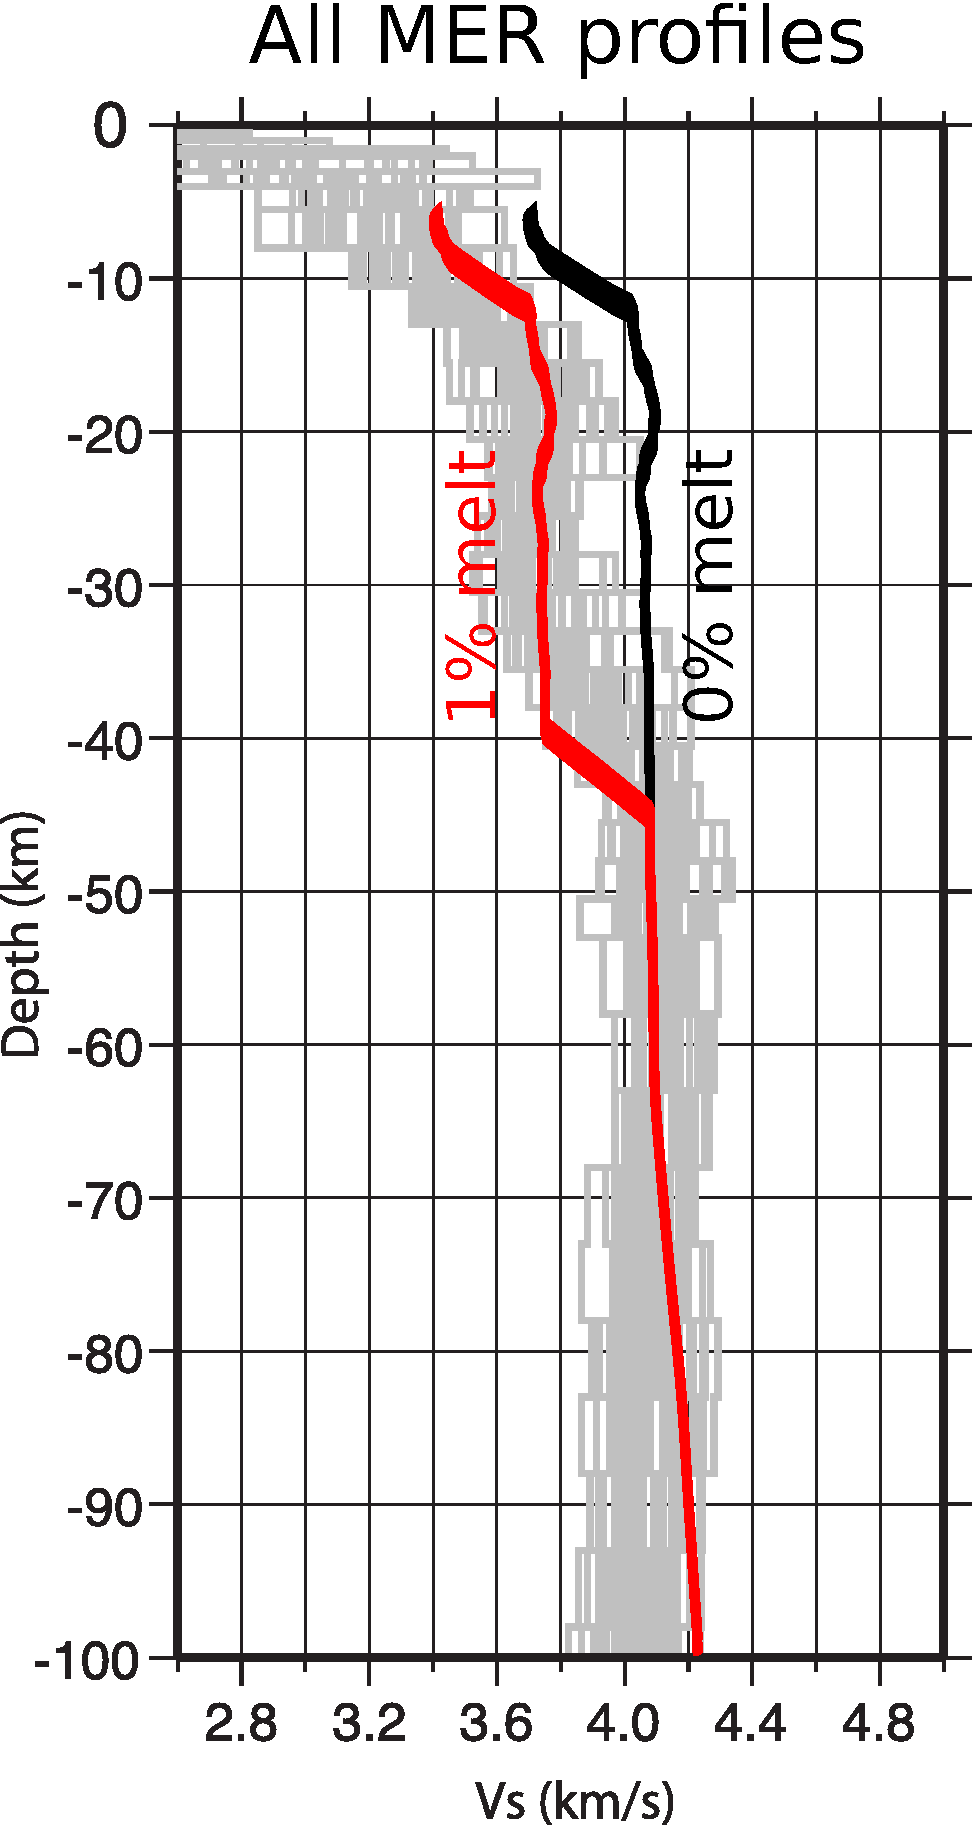
\includegraphics[height=0.5\paperheight]{./figures/MER2.png}
        \caption{Comparison of the predicted S-wave seismic velocity from the forward model and the ensemble vertical
                 profiles from the joint inversion of Rayleigh waves and receiver functions below the Main Ethiopian Rift
                 \citep{keranen-etal-2009}. The black line is the model $V_{S}$ assuming no melt storage, the red line
                 assumes that 1\,\% melt is stored above 40\,km depth.}
    \end{figure}
\end{frame}

\subsection{Melt transport}

\begin{frame}
    \frametitle{Part 1.3: Melt transport and deglaciation}
    \begin{figure}
        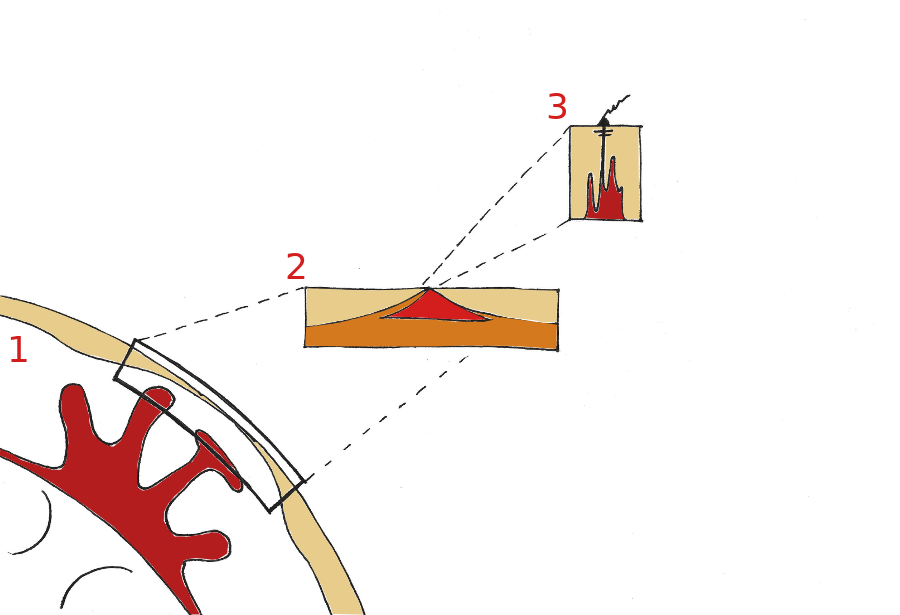
\includegraphics[height=0.9\paperheight]{./pictures/drawing.png}
    \end{figure}
\end{frame}

\begin{frame}
    \frametitle{Melt retention and melt velocity: a trade off}
    \begin{figure}
        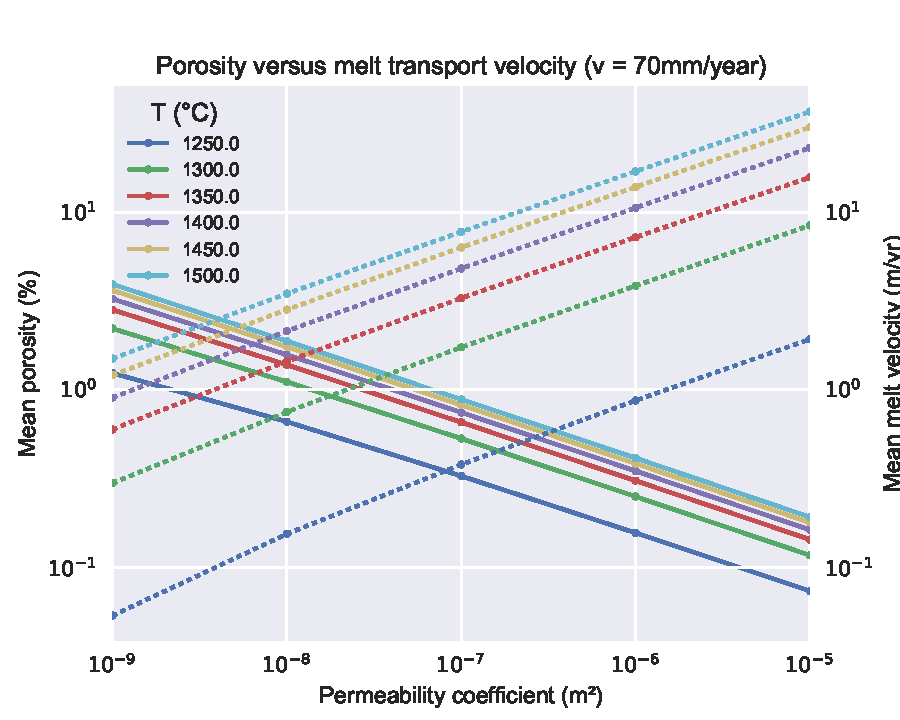
\includegraphics[height=0.7\paperheight]{./figures/ch2-phi-vm.pdf}
        \caption{To have high melt retention requires slow melt transport \citep{franken-etal-2020}. However, it is
                 often reported that melt generation responds to climatic forcing.}
    \end{figure}
\end{frame}

\begin{frame}
    \frametitle{Iceland: Melt generation since last glacial maximum (LGM)}
    \begin{figure}
        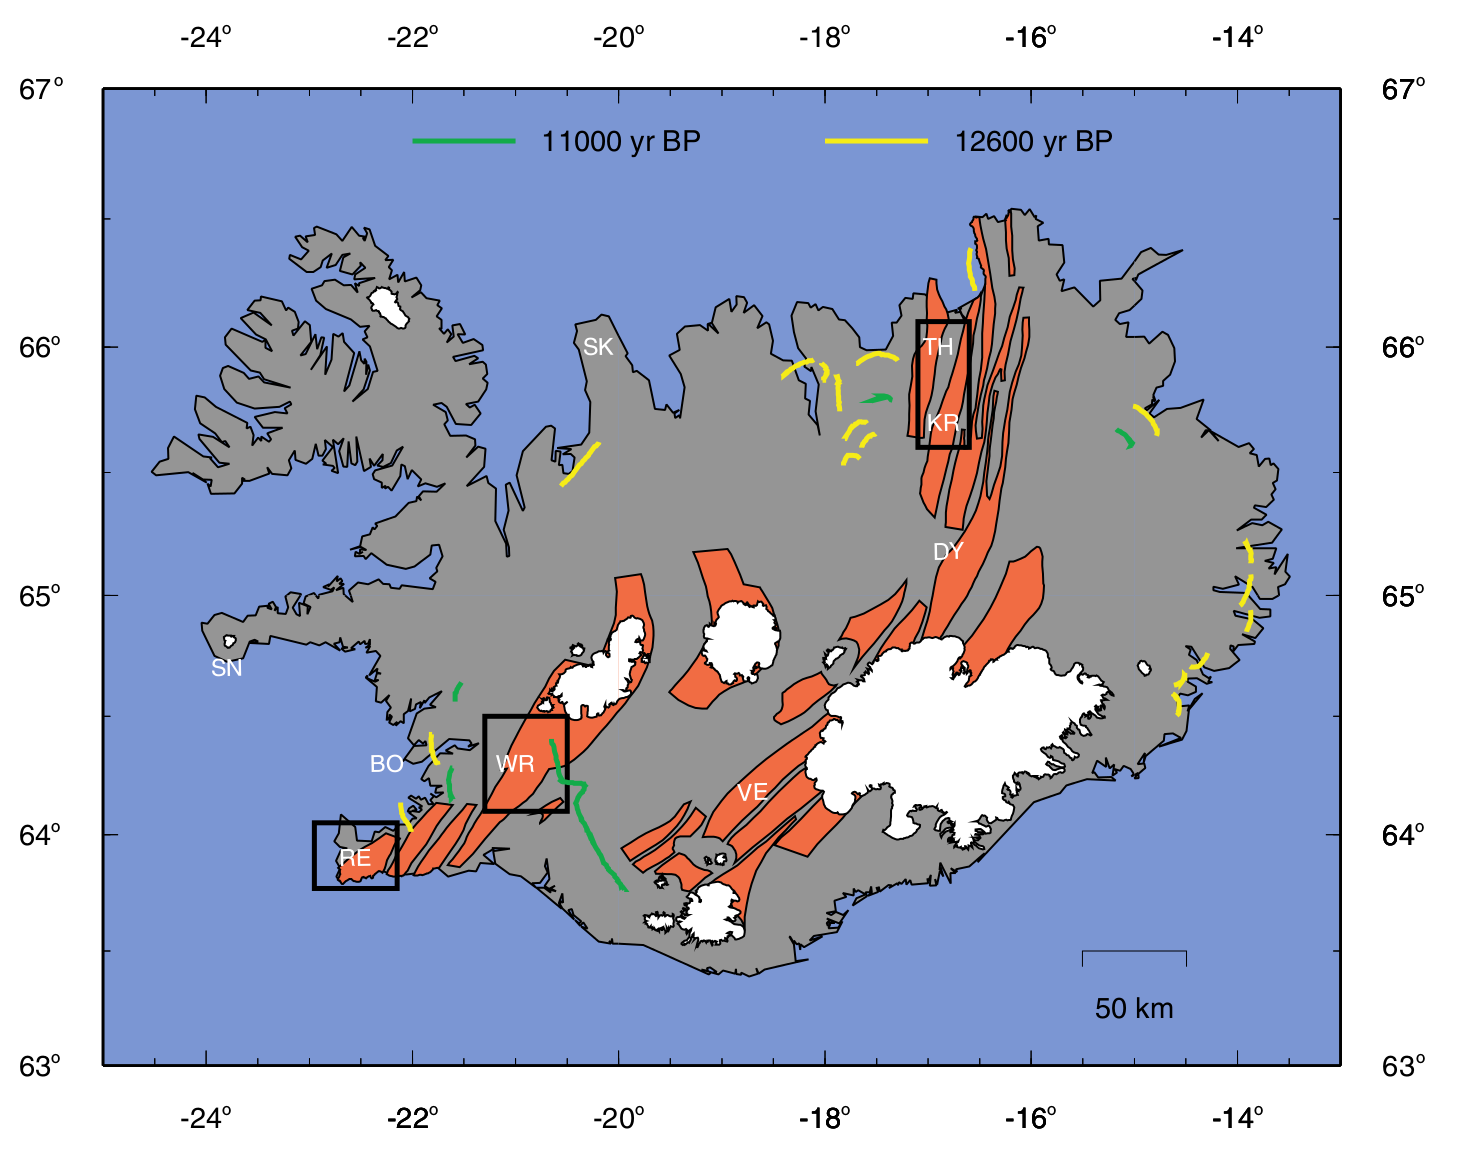
\includegraphics[height=.65\paperheight]{./figures/iceland-map.png}
        \caption{Distribution of basalt flows and limits of ice-sheet \citep{maclennan-etal-2002}}
    \end{figure}
\end{frame}

\begin{frame}
    \frametitle{Iceland: Melt generation since last glacial maximum (LGM)}
    \begin{columns}
        \begin{column}{0.4\textwidth}
            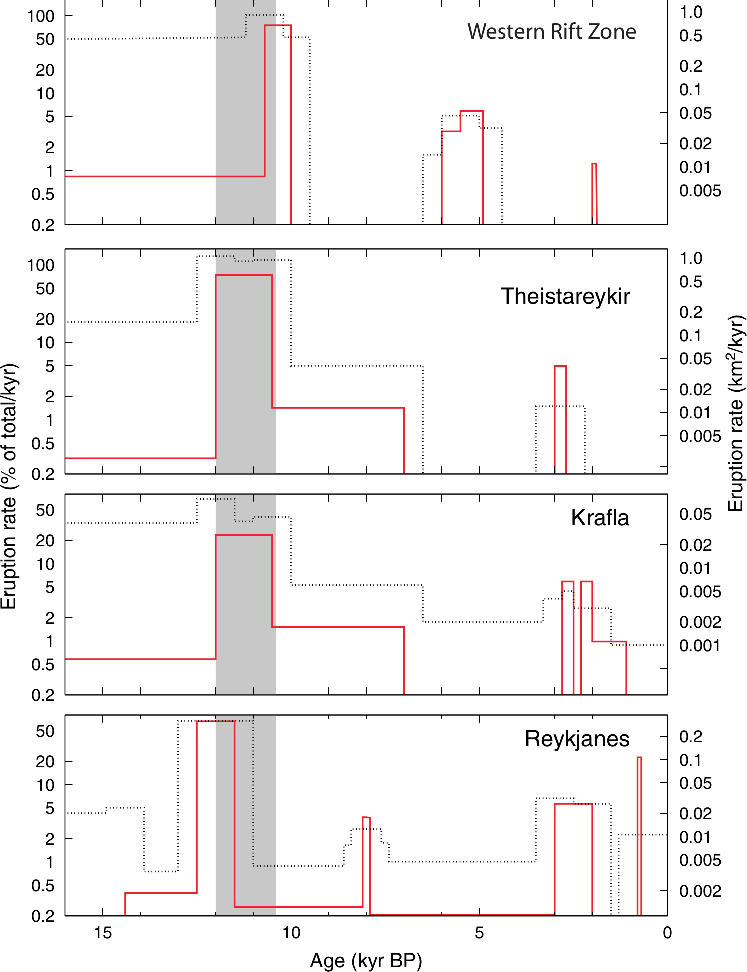
\includegraphics[height=.8\paperheight]{./figures/iceland-volumes.pdf}
        \end{column}
        \begin{column}{0.6\textwidth}
            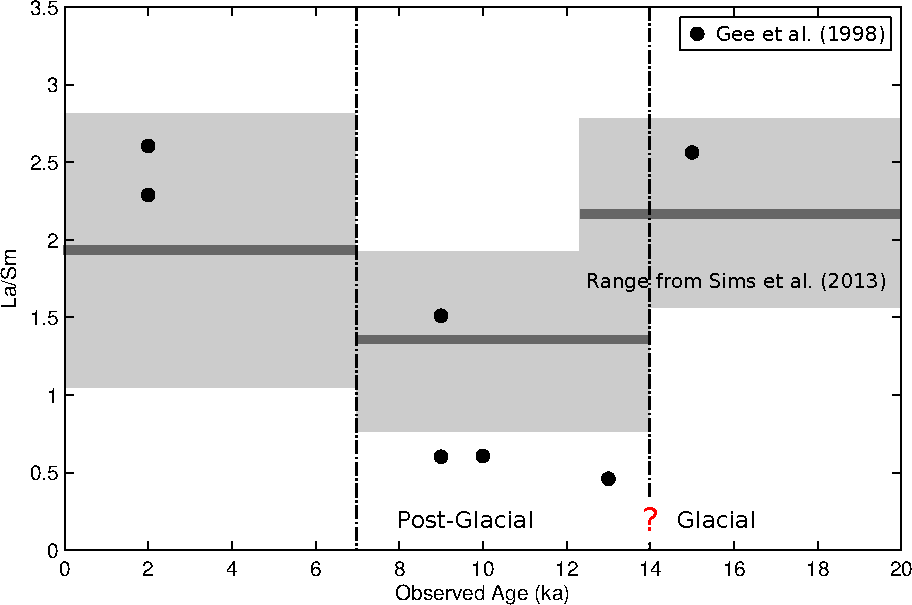
\includegraphics[height=.5\paperheight]{./figures/iceland-chemistry.pdf}
            Change in La and Sm concentrations since LGM. Low La/Sm due to increased shallow melt production?
        \end{column}
    \end{columns}
\end{frame}

\begin{frame}
    \frametitle{Solve for vertical flow of melt}
    \begin{columns}
        \begin{column}{0.5\textwidth}
            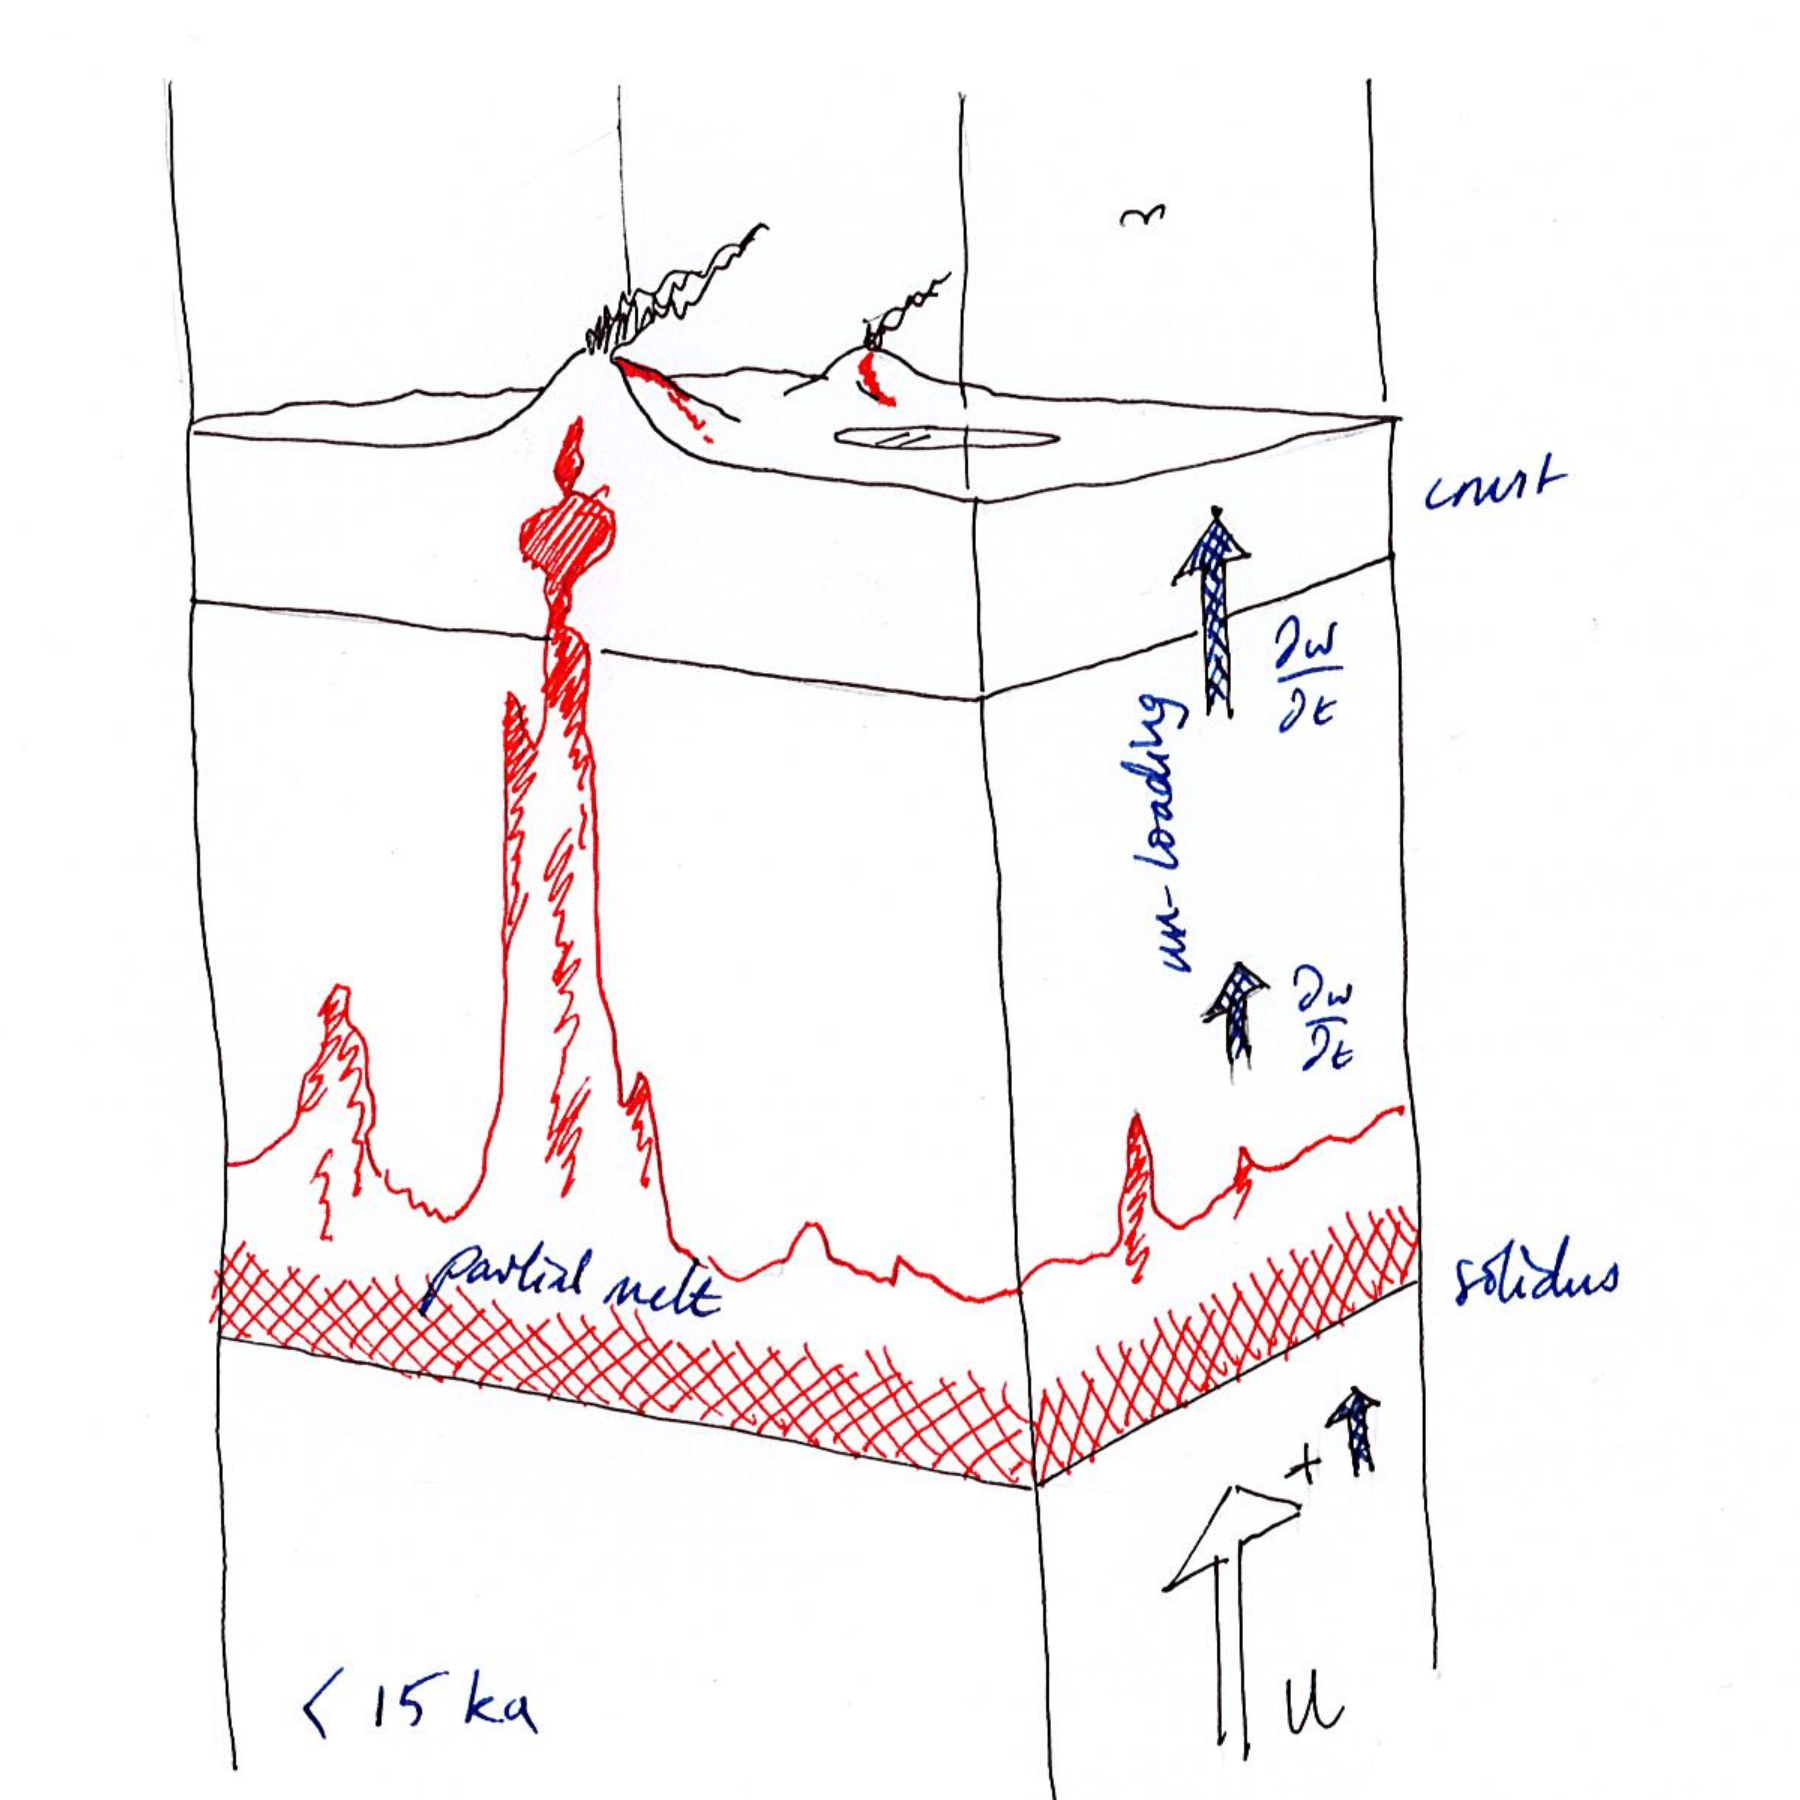
\includegraphics[width=.45\paperwidth]{./figures/sketch1b.png}
        \end{column}
        \begin{column}{0.5\textwidth}
            Define an average velocity,\newline
            \[
            \bar{v} = (1-\phi)v_{s} + \phi v_{l},
            \]
            and this velocity is given by the rate of up-welling plus the rate of change of displacement due to loading (unloading),\newline
            \[
            \bar{v} = u + \frac{\partial w}{\partial t},
            \]
            where $u$ is the rate of up-welling.
        \end{column}
    \end{columns}
\end{frame}

\begin{frame}
    \frametitle{Solve for vertical flow of melt}
    \begin{columns}
        \begin{column}{0.5\textwidth}
            \includegraphics[width=.45\paperwidth]{./figures/sketch1a.png}
        \end{column}
        \begin{column}{0.5\textwidth}
            \[
            \bar{v} = u + \frac{\partial w}{\partial t},
            \]
            where $\partial w/ \partial t$ is the rate of change in vertical displacement. This is calculated from the change in surface displacement, $w_{0}$,
            \[
            \frac{ET_{e}}{12\left(1-\mu^{2}\right)} \frac{\partial^{4}}{\partial x^{4}}\left(\frac{\partial w_{0}}{\partial t}\right) = \frac{P_{ice}}{\tau_{e}},
            \]
            $P_{ice}$ is the load due to an ice-sheet, and $\tau_{e} = 3\eta_{s}/E$ is the viscous response time.

            This displacement decays with depth as,
            \[
            \frac{\partial w}{\partial t} = \frac{\partial w_{0}}{\partial t}exp\left(-\sqrt{3}\pi\frac{z}{\lambda}\right),
            \]
            where $\lambda$ is the width of the ice-sheet.
        \end{column}
    \end{columns}
\end{frame}

\begin{frame}
    \frametitle{Solve for vertical flow of melt}
    \begin{columns}
        \begin{column}{0.5\textwidth}
            \includegraphics[width=.45\paperwidth]{./figures/sketch1a.png}
        \end{column}
        \begin{column}{0.5\textwidth}
            Conservation of energy,\newline
            \[
            mL + \frac{\partial T}{\partial t} + \bar{v}\frac{\partial T}{\partial z} - \kappa\frac{\partial^{2} T}{\partial z^{2}} = 0.
            \]
            Conservation of mass for the melt,\newline
            \[
            \frac{\partial\phi}{\partial t} + \frac{\partial}{\partial z}\left(\phi v_{l}\right) = m.
            \]
            Darcy's law (assuming zero-compaction length),\newline
            \[
            \phi\left(v_{l}-v_{s}\right) = \frac{k_{0}\phi^{n}}{\eta_{l}}\Delta\rho g.
            \]
        \end{column}
    \end{columns}
\end{frame}

\begin{frame}
    \frametitle{Solve for vertical flow of melt}
    \begin{columns}
        \begin{column}{0.5\textwidth}
            \includegraphics[width=.45\paperwidth]{./figures/sketch1b.png}
        \end{column}
        \begin{column}{0.5\textwidth}
            Use the definition of average velocity, Darcy's law,\newline
            \[
            \phi\left(v_{l}-v_{s}\right) = \frac{k_{0}\phi^{n}}{\eta_{l}}\Delta\rho g,
            \]
            assuming $n=3$, and conservation of mass to get,\newline
            \[
            \frac{\partial\phi}{\partial t} + \bar{v}\frac{\partial\phi}{\partial z} + \frac{3k_{0}\Delta\rho g}{\eta_{l}}\phi^{2}\left(1 - \frac{4}{3}\phi\right)\frac{\partial\phi}{\partial z} = m.
            \]
            We have one unknown, $\phi$, where melt production rate $m$ is calculated from the temperature difference to the solidus.
        \end{column}
    \end{columns}
\end{frame}

\begin{frame}
    \frametitle{Impact of permeability on melt storage and simulated seismic velocity}
    \begin{figure}
        \includegraphics[height=0.7\paperheight]{./figures/iceland-profiles.png}
        \caption{Profiles of porosity and seismic velocity for the 1D model.}
    \end{figure}
\end{frame}

%\begin{frame}
%    \frametitle{Simulated melt eruption rates for the Pleistocene}
%    \begin{figure}
%        \includegraphics[height=0.7\paperheight]{./figures/iceland-model1.png}
%        \caption{For the model to respond rapidly to deglaciation the permeability coefficient needs to be high, $k_{0}=10^{-5}$}
%    \end{figure}
%\end{frame}

\begin{frame}
    \frametitle{Simulated melt eruption rates for the Holocene}
    \begin{figure}
        \includegraphics[height=0.7\paperheight]{./figures/iceland-response.png}
        \caption{For the model to respond rapidly to deglaciation the permeability coefficient needs to be high, $k_{0}=10^{-5}$}
    \end{figure}
\end{frame}

\begin{frame}
    \frametitle{Simulated melt eruption rates for the Holocene}
    \begin{figure}
        \includegraphics[height=0.7\paperheight]{./figures/iceland-model2.png}
        \caption{For the model to respond rapidly to deglaciation the permeability coefficient needs to be high, $k_{0}=10^{-5}$}
    \end{figure}
\end{frame}

%\begin{frame}
%    \frametitle{Simulated melt eruption rates for the Holocene}
%    \begin{figure}
%        \includegraphics[width=0.9\paperwidth]{./figures/iceland-all.png}
%        \caption{Response is reflected in the trace element record and there is a interesting relationship to CO$_{2}$ fluxes}
%    \end{figure}
%\end{frame}

\begin{frame}
    \frametitle{Melt retention and melt velocity: a trade off}
    \centering
    \includegraphics[height=0.7\paperheight]{./figures/ch2-phi-vm.pdf}
\end{frame}

\begin{frame}
    \frametitle{Visoc-elasto-plastic model to seismic structure}
    \begin{figure}
        \includegraphics[height=0.5\paperheight]{./figures/MER2.png}
        \caption{The black line is the model $V_{S}$ assuming no melt storage, the red line
                 assumes that 1\,\% melt is stored above 40\,km depth, {\bf but how can we both have high storage and fast transport?}}
    \end{figure}
\end{frame}

\begin{frame}
    \frametitle{Questions not conclusions}
    \begin{itemize}
        \item[-]{We cannot have both a system that responds to climate change and stores melt.}
        \item[-]{What if the model of McKenzie for the compaction and transport of melt is not appropriate?}
        \item[-]{Does melt flow localise into channels, flow like rivers through the matrix?}
    \end{itemize}
\end{frame}

\section{Part 2: Rivers}

{
\usebackgroundtemplate{\includegraphics[width=\paperwidth]{./pictures/rivers.png}}
\begin{frame}
    \frametitle{Part 2: Rivers}
\end{frame}
}

\begin{frame}
    \frametitle{Width of a river relative to the width of a cell}
    \centering
    \includegraphics[height=0.9\paperheight]{./figures/flem-grid.png}
\end{frame}

\begin{frame}
    \frametitle{Width of a river relative to the width of a cell}
    \centering
    \includegraphics[height=0.6\paperheight]{./figures/river-width.png}
    \begin{itemize}
        \item[-]{Distribution of mean river width taken from the Global River Widths from Landsat (GRWL) Database \citep{allen-2018}}
        \item[-]{How do we model the transport of sediment by flowing water? At a scale smaller or larger than a river?}
    \end{itemize}
\end{frame}

\begin{frame}
    \frametitle{A landscape evolution model}
    One of the simplest landscape evolution models can be derived if we assume erosion and deposition occur due to the
    transport of sediment across the surface of the Earth.
    \[
    \frac{\partial z}{\partial t} = \nabla{\mathbf{q_{s}} + U}
    \]
    and that sediment flux is a function of the water flux,
    \[
    \mathbf{q_{s}} = - \left[\kappa \nabla{z} + c \mathbf{q_{w}} \cdot \nabla{z}\right]
    \]
    but how to route water?
    \includegraphics[width=0.8\paperwidth]{./figures/MFDandSFD.png}
\end{frame}

\begin{frame}
    \frametitle{Single Flow Direction (SFD; steepest descent) cell to cell}
    \centering
    \includegraphics[height=1cm]{./figures/MFDandSFD.png}
    \includegraphics[height=0.8\paperheight]{./figures/flem-sfd-c2c.png}
\end{frame}

\begin{frame}
    \frametitle{Single Flow Direction (SFD; steepest descent) node to node}
    \centering
    \includegraphics[height=1cm]{./figures/MFDandSFD.png}
    \includegraphics[height=0.8\paperheight]{./figures/flem-sfd-n2n.png}
\end{frame}

\begin{frame}
    \frametitle{Multiple Flow Direction (MFD; distributed) cell to cell}
    \centering
    \includegraphics[height=1cm]{./figures/MFDandSFD.png}
    \includegraphics[height=0.8\paperheight]{./figures/flem-mfd-c2c.png}
\end{frame}

\begin{frame}
    \frametitle{Multiple Flow Direction (MFD; distributed) node to node}
    \centering
    \includegraphics[height=1cm]{./figures/MFDandSFD.png}
    \includegraphics[height=0.8\paperheight]{./figures/flem-mfd-n2n.png}
\end{frame}

\begin{frame}
    \frametitle{Valley to valley wavelength}
    \centering
    \includegraphics[height=0.9\paperheight]{./figures/wavelength.png}
\end{frame}

\begin{frame}
    \frametitle{Sediment flux through time}
    \centering
    \includegraphics[height=0.9\paperheight]{./figures/sediment-flux.png}
\end{frame}

\begin{frame}
    \includegraphics[width=0.8\paperwidth]{./figures/MFDandSFD.png}
    \begin{itemize}
        \item[-]{MFD node-to-node resolves the resolution dependence}
        \item[-]{The flow of water is therefore being treated as going down 1D lines distributed over multiple (<6) directions}
        \item[-]{Most LEMs assume a single flow direction as it is expedient, but water does not flow down slope in such a simple manner.}
        \item[-]{Should LEMs start to consider how water really flows through the landscape?}
    \end{itemize}
\end{frame}

\section{Rivers and Melt}

\begin{frame}
    \frametitle{Rivers and Melt}
    \begin{itemize}
        \item[-]{In both parts, melt transport and landscape evolution, the models are on a scale far greater than the processes.
                 Simplifying assumptions must be made. Yet in both cases the physics of the processes at a scale below the model grid cannot be ignored.}
        \item[-]{Classic Darcy flow through a permeable matrix cannot explain the ensemble of observations: \newline
                 \textit{the seismic observations tend to require a longer travel time delay that can be explained by melt retention alone}}
        \item[-]{Landscape evolution models cannot overlook processes at the scale of a river: \newline
                 \textit{we need to numerically distribute the water to all down slope cells, but in nature water flows through the landscape not on top of it.}}
        \item[-]{It is only by comparing the models with observations that the importance of these processes becomes clear.}
    \end{itemize}
\end{frame}

\section{What next?}

\begin{frame}
    \frametitle{What next: Groundwater}
    \includegraphics[width=0.9\paperwidth]{./figures/{groundwater.svg}.png}
\end{frame}

\begin{frame}
    \frametitle{Surface and groundwater}
    \begin{itemize}
        \item[-]{Roughly 40\,\% of water is transported in the subsurface. This transport is not captured by landscape evolution models.}
        \item[-]{In steep and high mountain catchments this store of water is of vital importance}
    \end{itemize}
    \centering
    \includegraphics[width=0.6\paperwidth]{./pictures/graphic1.png}
\end{frame}

\begin{frame}
    \frametitle{Passive seismic monitoring of groundwater}
    \begin{itemize}
        \item[-]{Focus on the Bhote Koshi catchment in Nepal}
    \end{itemize}
    \centering
    \includegraphics[height=0.6\paperheight]{./figures/illien-figure.png}
\end{frame}

\begin{frame}
    \frametitle{Passive seismic monitoring of groundwater}
    \begin{itemize}
        \item[-]{Change in the groundwater levels is reflected in the cross-correlation of ambient seismic noise \citep{illien-etal-2021}}
    \end{itemize}
    \centering
    \includegraphics[height=0.7\paperheight]{./figures/illien-figure2.png}
\end{frame}

\begin{frame}
    \frametitle{PhD project starting in December}
    \begin{itemize}
        \item[-]{Develop methods to couple surface and groundwater flow}
        \item[-]{Use existing observations from Nepal to explore model assumptions and hypothesis}
        \item[-]{Collaboration with Niels Hovius, Christoff Andermann, and Nobu Fuji}
    \end{itemize}
    \vspace{0.5cm}
    \includegraphics[width=0.9\paperwidth]{./figures/{groundwater.svg}.png}
\end{frame}

\begin{frame}
    \frametitle{References}
    {\tiny
    \bibliographystyle{elsart-harv}
    \bibliography{ref}
    }
\end{frame}

\end{document}
